%% !TeX root = IIII_simulator
% !TeX root = article

% Disallow floats on the first page
\suppressfloats

%Design, notation and application

\title{Real-Time Synthetic Aperture Sonar Simulation for Automatic Target Recognition: Notation and Application}

\author{{Jo~Inge~Buskenes, %
        Herman~Midelfart%, %
%        \O{}ivind~Midtgaard
        } %
\thanks{J. I. Buskenes is with both the Department of Informatics, University of Oslo, Norway, and the Norwegian Defense Research Establishment (FFI), Norway.}%
\thanks{H. Midelfart and \O. Midtgaard are with The Norwegian Defence Research Establishment (FFI), Norway.}% <-this % stops a space
% \thanks{Manuscript received April 19, 2005; revised January 11, 2007.}
}

% The paper headers
\markboth{IEEE Journal of Oceanic Engineering}%
{A GPU Sonar Simulator for Automatic Target Recognition}


% Publishers ID mark:
%\IEEEpubid{0000--0000/00\$00.00~\copyright~2007 IEEE}

% use for special paper notices
%\IEEEspecialpapernotice{(Invited Paper)}

% for Computer Society papers, we must declare the abstract and index terms
% PRIOR to the title within the \IEEEcompsoctitleabstractindextext IEEEtran
% command as these need to go into the title area created by \maketitle.
\IEEEcompsoctitleabstractindextext{%
\begin{abstract}
\todo{Revise abstract, and make a point of the notation system}Template matching is a common technique for automatic classification of objects in synthetic aperture sonar (SAS) images. The principle is to isolate an image segment containing the object of interest, correlate it with a set of template images, and assign it to the class of the template yielding the highest correlation coefficient. The challenge is to come up with a representative set of template images covering the relevant configurations of object and seabed.

We target this challenge with a sonar simulator that first takes as input a seabed model derived from the real sonar image. Then it places a 3D object model on the seabed, renders the scene, and adds the resulting image to the template set. For every object type, position, alignment and material, the procedure is repeated, and a correlation coefficient computed. The best performance is obtained when these parameters are estimated from the sonar image as part of the classification process. The simulator is therefore written in OpenGL and OpenCL and runs on graphics processing units (GPUs). The result is a fast performing and portable template generator which can adapt to the characteristics of the current scene on-the-fly.
\end{abstract}

% Keywords (normally not used for peer reviews)
\ifPeerReview\else
\begin{IEEEkeywords}
Sonar, SAS, simulator, template matching, OpenGL, OpenCL.
\end{IEEEkeywords}
\fi}
% \fi 

% make the title area
\maketitle

% This command fixes abstract positioning for compsoc articles:
\IEEEdisplaynotcompsoctitleabstractindextext

% (Optional) Add some extra info on cover page of peer review papers:
% \ifCLASSOPTIONpeerreview
% \begin{center} \bfseries EDICS Category: 3-BBND \end{center}
% \fi

% Insert page break and insert second title (peer review mode)
\IEEEpeerreviewmaketitle



\section{Introduction}

\setcounter{totalnumber}{1}
\setcounter{topnumber}{1}
\setcounter{dbltopnumber}{1}

\providecommand\cancel{}\renewcommand\cancel[2][char]{%
% % \tikzmark{#1}{$#2$}%
% \tikz[font=\scriptsize,overlay,baseline=(char.base)]{%
\tikz[font=\scriptsize]{%
\node[inner sep=0pt](#1){$#2$};%
\begin{scope}[overlay]%
\coordinate(offsett) at (0.3em,1.2ex);%
\draw[-] ($(#1.center) - (offsett)$) to ($(#1.center) + (offsett)$);%
\end{scope}%
}
}


\providecommand\m*{}\renewcommand*\m[2][\phantom{jf}]{\tikzmark{#2}{#1}}
\providecommand\k*{}\renewcommand*\k[2]{{\scriptsize\color{black}\tikzmark{#1}{$#2$}}}
\providecommand\g*{}\renewcommand*\g[2]{{\scriptsize\color{Green}\tikzmark{#1}{$#2$}}}
\providecommand\r*{}\renewcommand*\r[2]{{\scriptsize\color{Red}\tikzmark{#1}{$#2$}}}
\providecommand\b*{}\renewcommand*\b[2]{{\scriptsize\color{blue}\tikzmark{#1}{$#2$}}}

% \draw[-{Latex[length=.5em,width=.5em]}]
%                         ($(C.center) + (offset) + (1.3em,-0.4ex)$) to[out=-30, in=90] ($(XC) + (offset) + (1.6em,0ex)$)
%       to[out=-90, in=0] ($(X.center) + (offset) + (0.8em,0ex)$);

\newlength\tpad\setlength\tpad{.2ex}
%\begin{tikzpicture}
%\coordinate(__) at ($ (0em,0ex) $);
%\end{tikzpicture}


% \newcommand\figstep[2]{\raisebox{.5pt}{\textcircled{\raisebox{-.9pt}{\textbf{\Green{#1}}}}}\mbox{}\hfill\parbox[t]{.97\linewidth}{#2}}
\newcommand\step[1]{\tikz[baseline=(char.base)]{%
            \node[shape=circle,draw,color=Green,inner sep=0.5pt] (char) {#1};}}
\newcommand\figstep[2]{\step{#1}\mbox{}\hfill\parbox[t]{.97\linewidth}{#2}} 
\begin{figure*}[t]\centering%
\ifOverLeaf%
  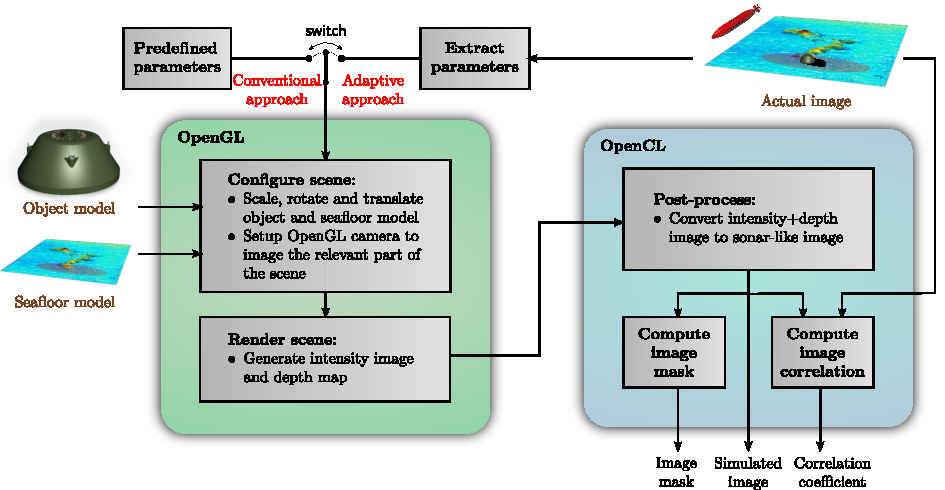
\includegraphics[width=\linewidth]{gfx/simulator.pdf}%
\else
  \includegraphics[drawing,width=\linewidth]{gfx/simulator.svg}%
\fi
\caption{\emph{Simulator concept}: Given as input 3D models of the object and seafloor, and some parameters for these, the simulator produces an image template, mask and a correlation coefficient. The \emph{conventional} (static) approach pick parameters from a predefined set, whereas the \emph{adaptive} approach estimate them from the sonar image. The implementation reside entirely on the GPU, with OpenGL performing scene rendering and OpenCL general-purpose post-processing. Compared to a CPU, the GPU's superior processing speed allow a much wider range of object parameters to be searched for an optimal template, yielding better results in a lesser time.}\label{IV_buildup}%
\end{figure*}

% \newcommand\figstep[2]{\raisebox{.5pt}{\textcircled{\raisebox{-.9pt}{\textbf{#1}}}}\mbox{}\hfill\parbox[t]{.97\linewidth}{#2}}
\begin{figure*}[t]\centering%
\ifOverLeaf%
  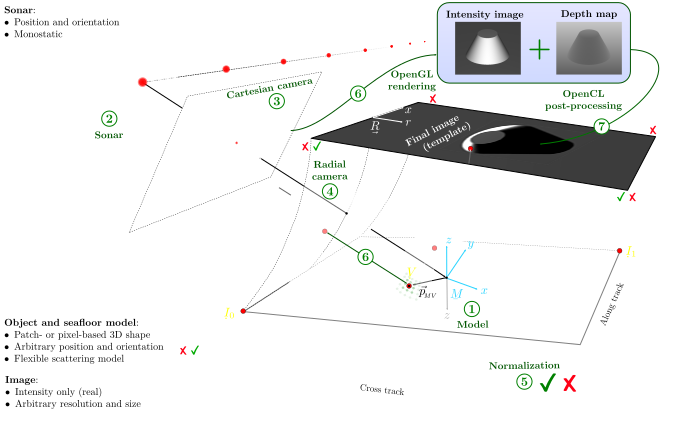
\includegraphics[width=\linewidth]{gfx/scene_coordinate_system_radial.pdf}%
\else
  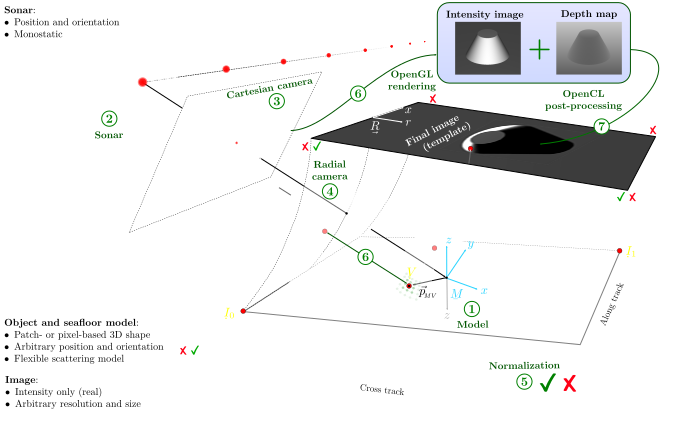
\includegraphics[width=\linewidth]{gfx/scene_coordinate_system_radial.svg}%
\fi
\caption[caption]{\emph{Virtual scene geometry and processing steps.} As marked with encircled numbers in the figure, five steps are needed to obtain the sonar template:\\[.5\baselineskip]
%
\figstep{1}{\emph{Model displacement.} When the 3D models of seafloor and object are loaded into OpenGL they each have their own reference frame $\protect\ubar{M}$. The region we seek to image has a position and orientation $\ubar{I}$. We apply the displacement (translation and rotation) of $\ubar{M}$ relative to $\protect\ubar{I}$ with a \emph{model matrix} $\mat{T}_\textit{\tiny\!IM}$.
}\\[.5\baselineskip]
%
\figstep{2}{\emph{Sonar translation.} The sonar local body has the reference frame $\ubar{S}$. Its orientation is equal to that of the image, $\uvec{S}=\uvec{I}$. We apply the remaining translation of $\udot{I}$ relative to  $\udot{S}$ with a \emph{sonar matrix} $\mat{T}_\textit{\tiny\!SI}$.
}\\[.5\baselineskip]
%
\figstep{3}{\emph{Orthogonal view rotation.} We want to position the OpenGL camera at the origin of the sonar frame, $\udot{S}$, looking at (i.e. $\hat{z}_O$-axis pointing at) the origin of the image frame, $\udot{I}$. While the  position is correct after step 2, we must apply the rotation of $\uvec{S}$ relative to $\uvec{O}$ with an \emph{orthogonal view matrix} $\mat{T}_\textit{\tiny\!SI}$.
}\\[.5\baselineskip]
%
\figstep{4}{\emph{Coordinate conversion.} The $\hat{x}_O$ and $\hat{y}_O$ axes span an orthogonal viewing plane onto which the scene's points can be projected. However, to simplify the boundary specification of range and elevation in the next step, we convert the coordinate representation from cartesian $(\hat{y}_O,\hat{z}_O)$ to cylindrical $(\hat{\phi}_C,\hat{r}_C)$ with a non-linear function T$_{CO}$.
}\\[.5\baselineskip]
%
\figstep{5}{\emph{Projection}. OpenGL only renders coordinates that fall in the range $[-1,1]$. We map the coordinate boundaries (for along-track, range and elevation) into this normalized range with a \emph{projection matrix} $\mat{T}_\textit{\tiny\!XC}$.
% 
% The size of this plane is determined by the desired image region on the seafloor. The projection is performed with the \emph{projection matrix} $\mat{T}_\textit{\tiny\!C}$.
}\\[.5\baselineskip]
%
\figstep{6}{\emph{OpenGL rendering.} When OpenGL renders the scene it uses a \emph{vertex shader} to apply our transformation matrices to every vertex, and a \emph{fragment shader} to compute the intensity values for each point in the image. OpenGL computes the range from each image pixel to its corresponding model facet: This is called a \emph{depth map}.
}\\[.5\baselineskip]
%
\figstep{7}{\emph{OpenCL post-processing.} Finally, the sonar-like image is formed---for some unique azimuth coordinate---by accumulating all intensity values that share the same range. This is our template. %  along with the depth information is finally combined to form a sonar like image. This is our template.
}%
}\label{IV_simulator_coordinate_system}%
\end{figure*}




% \IEEEPARstart{W}{hen} 
% Autonomous underwater vehicles (AUVs). When an AUV with a sonar imaging system encounter an interesting object, it would be very beneficial if adapted its behavior to examine the object further. This is challenging as it would need to learn in what ways the interesting objects differ from the background, i.e. it relies on previous knowledge. It would also need to process this information is near real-time to act in an efficient manner.

% - Adapt simulation to its behaviour, see if they still match.


\IEEEPARstart{A}{utonomous} underwater vehicles (AUVs) are vital in the exploration of our underwater frontiers. When equipped with a modern synthetic aperture sonar (SAS), they map seafloors, survey underwater biology, help localize wrecks, inspect oil pipes, fields and electricity lines, or help remove mines, biohazard waste or plastic. However, they struggle to deal with unforeseen events, such as poor imaging conditions, blocked paths, corrupted data or rare objects. One reason is their lack of a reliable and adaptive system for automatic target recognition (ATR).

%However, Such independent systems have much to gain from being able to adapt to the scenario at hand. For instance, with a well designed automatic target recognition (ATR) system on board they can adapt their mission plan to collect more information on particularly interesting objects, or fine-tune the sonar and navigation system to create better images.
 
% Automatic target recognition (ATR) is an important component in autonomous underwater vehicles (AUVs), as it allows the vehicle to adapt its mission plan to e.g. revisit detected objects for closer examination. One way to classify these objects is by using template matching. The principle involved  is to isolate an image segment containing the object of interest, compare it with a set of template images of the relevant object classes, and assign it to the class of the template with the the best fit.

A conventional ATR system isolates an object of interest, extracts its key features, and uses these to estimate the object's class. The challenge is to find features that are unique and intrinsic, such as type, shape and size, independent of extrinsic ones such as alignment, burial depth, degeneration level or view angle. Such features are rare in SAS, despite its best-in-class resolution and dynamic range, due to image ambiguities from acoustical distortions such as layover, multiple scattering, diffraction, dispersion and penetration.

%Thus, the sonar image contains incomplete object information, and only contains partial object can only describe the object partially, can't be used to infer the object class unambiguously.


%
%Information is lost in the 
%
%Inferring the object class from the sonar image ambiguous, the sonar image ambiguous,  sonar image an ambiguous and suboptimal source to infer the object class from.

% This makes the sonar image represent the object ambiguously, and makes the class estimation unreliable.\todo{Not happy with this sentence}



%
%Object information is partially lost in the process, 
%
%Inferring object class from incomplete information.
%
%Since object information is lost in the process, 

%
%Thus, the sonar image ambiguously represent the object class Thus, the object class 
%
%
%Object ambiguously represented by the sonar image, and can't be inferred from it reliably.
%
%Sonar image represent the object ambiguously, making inference of 
%Inferring the object class from the sonar image is difficult, because it 
%
%Information is lost making the sonar image ambiguous, and inferring the object class hard.
%

%As a result the sonar image provide an ambiguous representation of the object.

%Information lost
%Sonar image ambiguous
%Inferring object class hard. 

% ambiguouslyInformation is lost in the process, preventing the object class can not be inferred unambiguously from the sonar image  The sonar image ambiguously describes the object class, and object class Inferring the object class from the sonar Information is partially lost in the process, making the sonar image an ambiguous representation of the object.\todo{bloated?}

%Inferring the object class from the sonar image

%Object information is irrevocably lost in the process, thus can no be inferred reliably from and  The resulting image e process is irreversible; No amount of guesswork To interpret and extract the needed information from these The image sought after may not be there, or take a form inconcievable for humans.

% Ideal parameters are unique and intrinsic---such type, shape, and size---, and independent of extrinsic features such as alignment, burial depth, degeneration level, or view angle.



 

%The challenge is to find unique and intrinsic object properties, such as type, shape and size, independent of extrinsic properties such as alignment, burial depth, degeneration level or view angle. 

%  comparable to optical cameras, but are harder to interpret; Acoustic effects such as layover, multiple scattering, diffraction, dispersion and penetration distort the image, making it an ambiguous representation of the object.

% Instead of trying to To bypass the intricacies of identifying a 3D object from an ambiguous 2D image, 

% Say how the templates come into existence first

% Instead of inferring object class from image, make a guess and compare simulation.

%Template matching bypass the problem of inferring the object class from the image, by guessing which object it is, 

%1. 3D model
%2. Acoustic simulation
%3. 
%
%An alternative approach consists of computing image templates for each object and orientation that may be 

% An alternative, called template matching, compares...
% Template matching differs by comparing the object...

Template matching offers an alternative to feature extraction: to compare the object with image templates of relevant classes and orientations, and assign the object to the class that fits best. The problem is to find a set of templates that properly represent the objects. Too many templates are needed to densely sample each degree of freedom. Therefore, practical implementations resort to a few sparsely sampled features, ultimately yielding inaccurate results~\cite{Midelfart2010}.

%
%Numerous templates are required for each object, since every degree of freedom needed to describe it adds a dimension to the template solution space\todo{simplify}. 
%
%
%
%Feature for every degree of freedom - unmanageable 

% exponentially with every degree of freedom needed to represent the objects, adds number of templates needed to represent an object well grows exponentially with its number of degrees of freedom\todo{some way to simplify here?}.



% assuming similar sampling granularity of each parameter. 


%Template matching bypass the feature extraction by comparing the detected object with a set of simulated object templates, and assign it the class of the template with the best fit.\todo{reword somehow}  

%Template matching targets the ambiguity by instead starts with 3D models of relevant objects and orientations, simulates acoustic image templates for each, correlates them with detections\todo{vague} in the actual image, and estimates the class to be that of the template yielding the highest score.\todo{long, heavy, vague}   

%Template matching instead starts with 3D models acoustical image templates of probable objects and orientations, correlates them with detections\todo{vague} in the actual image, and estimates the class to be that of the template yielding the highest score.\todo{too heavy, vague} 

%Template matching instead starts with 3D models acoustical image templates of probable objects and orientations, correlates them with detections\todo{vague} in the actual image, and estimates the class to be that of the template yielding the highest score.\todo{too heavy, vague} 

%assigns records the scores. After iteration through all object classes and parameter configurations, the each detection is 

%roduce a template simulate how it would appears in a sonar image, and search the actual sonar image for similarities.  

%the deterministic acoustical effects distortions to produce an image template, and see if this resembles anything in the sonar image. This is called template matching.


%Template matching offers an alternative approach: Here an isolated image segment is compared to a set of template images covering the relevant object classes and orientations, and assigned to the class of the template with the best fit. Since the templates are computed from 3D models, this reduces the issue of image ambiguity. 

%However, it is challenging to find a static set of templates covering all suitable configurations of object and seafloor. Another issue is that the size of pre-computed library of templates grows exponentially with the number of parameters needed, assuming similar sampling granularity of each parameter. This limits its use to only a few parameters being coarsely sampled, ultimately yielding inaccurate results~\cite{Midelfart2010}.


% We avoid the problems of conventional template matching by computing the templates on-the-fly as part of the classification process, thereby not needing a precomputed set of templates at all. 
%  that avoids this problem by running sufficiently fast to create templates adapted to the actual scene as part of the classification process.
% Classification process


% Adaptive template matching:
% - To extract key features off the image

% Simulation of the templates:
% - To avoid static library of templates.
% - Less memory, better performance.


% To improve the reliability and efficiency, we propose two 
% reliability and efficient

%- AUV
%- ATR - feature extraction
%- ATR - template matching

%reduce feature solution space 

Adaptive template matching is a hybrid solution: to extract the most reliable statistics from the image, such as shadow and highlight characteristics, and use these to limit the template solution space~\cite{Midelfart2010}. This enables a fine-grained search through more features, at a reduced computational load and improved accuracy. However, we can remove a template library completely by simulating the templates on-the-fly.

%, to adapt to much broader scenarios.


% estimates some To overcome the limitation on In previous work we propose to adaptive  implement adaptive template matching using partial feature extraction. 
%We implement a hybrid solution by selecting a template based on object and seafloor parameters estimated from the SAS image~\cite{Midelfart2010}.
%
%We address the efficiency and problems of conventional template matching with \emph{adaptive template matching}---selecting a template based on object and seafloor parameters estimated from the SAS image~\cite{Midelfart2010};\todo{   **template selection based on object and seafloor parameters from SAS image***       Takes up a bit too much space, considering it won't be described in great detail} and
%\emph{real-time template simulation}---creating a template tailored to the estimated parameters, to improve its accuracy and avoid the need of a precomputed template library. 

%
%\todo{However, only a few simulators for high frequency, side-looking sonar imagery have been published. ***}
A few simulators for high frequency, side-looking sonar imagery have been published, e.g.~\cite{Bell1997,Sammelm2003}. We seek a fast simulator for creating simple templates, but most implementations prioritize accurate acoustic modeling at the expense of execution speed. One exception is the SIGMAS+ simulator~\cite{Coiras2009a, Coiras2009b}, which is accelerated by the parallel computing power of graphics processing units (GPUs). Aligning with our goals, it assumes Lambertian scattering and creates the sonar image from a 3D model with multiple renderings by the OpenGL computer graphics library. However, it includes stochastic effects such as ambient noise, which we deem irrelevant for templates, and its OpenGL-centric nature makes it suboptimal as an adaptive template matcher.

%while we consider templates deterministic. Neither is

%is intended for computer graphics; a side-effect of OpenGL due to the limitations of OpenGL, which is intended for computer graphics.

%It also relies on multiple  rendering passes to create the sonar image\\

% Since OpenGL is primarily intended for computer graphics, This is a drawback of OpenGL, which leaves a lot to be desired in terms of flexibility and extensibility---OpenGL is not a general-purpose programming tool.\todo{Trim, too verbose}

% - lack of flexibility
% - lack of extensibility

% - 
% This enables fast and flexible general-purpose computing on the GPU.
% This allows tailoring the sonar image with greater flexibility and allows tighter integration with the classifier.\todo{Too vague} 
% on a new full geometrical implementation of the simulator.

Our simulator was designed from the ground up to be part of a GPU-accelerated adaptive template matcher. It uses both OpenGL and the general-purpose programming framework OpenCL; two libraries that can inter-operate on the GPU. We describe it using a new notation system for homogeneous coordinates that allows complicated geometries to be expressed in a rigorous, unified and simple way. Its function is verified using data from Jesus Bay, Norway, recorded by the HISAS1030 100\,kHz SAS  mounted on a HUGIN AUV from Kongsberg Maritime.

%The simulator architecture and notation system are described Section~\ref{IV_methods}. Simulation and classification results  Results from  template simulations and classification Section~\ref{IV_results}  Finally, we present classification performance using 
%
%, and supply a Python snippet to demonstrate it.Section???
%In Section . 
%
%\todo{Introduce sections}

% Mathematical formulation/notation: Simulation, Robotics

%We will explore the classification performance of these two techniques, but otherwise 
%In this study we focus on describing the simulator, but compare classification results from both methods to that of standard template matching. 
% but provide some details on adaptive template matching for completeness where needed. 






%We will show that:
%%
%\begin{itemize}
%\item Adaptive template matching improves classification performance compared to its conventional peer,
%\item Improved classification performance by feeding simulator with parameters derived off SAS image,
%\item Further improved classification by performing a fine-search within a narrow search space around the SAS derived parameters. GPU makes this more powerful.
%\end{itemize}

% This is achieved with the aid of the massive computing power in graphics processing units (GPUs) and optimized software libraries for scene rendering. The simulator loads a 3D model of the seafloor and object class into OpenGL and positions the camera at the sonar location. The scene is highlighted using a light tube that extends to infinity along the AUV's axis of probagation. We assume rough, isotropic surfaces reflecting sound energy equally in all directions. This can be modeled with a Lambertian scattering model~\cite{Blake1993,Bell1995}, where the intensity of the backscattered sound solely depends on the incidence angle of the transmitted signal onto the model surface. The OpenGL rendering produces an optical 2D intensity image and depth map that reveals the distance from each pixel to the propagation axis. For maximum flexibility this data is finally combined with OpenCL to produce the image templates.

%as part of the classification process. This is achieved with the aid of the massive computing power in graphics processing units (GPUs) and optimized software libraries for scene rendering.

%The simulator loads a 3D model of the seafloor and an object class model into OpenGL, where emitted sound waves are modeled with a cylindrical light source placed at the sonar transmit location. 

%We assume rough, isotropic surfaces reflecting sound energy equally in all directions. This can be modeled with a Lambertian scattering model~\cite{Blake1993,Bell1995}, where the intensity of the backscattered sound solely depends on the incidence angle of the transmitted signal onto the model surface. When rendering OpenGL is set up to produce an optical 2D intensity image and depth map that reveals the distance from each pixel to the propagation axis. For maximum flexibility this data is finally combined with OpenCL to produce the image templates.


%For lack of a better name, the simulator will be referred to as "FFISim" throughout this article.

%



\section{Methods}\label{IV_methods}

%\begin{itemize}
%\item Unified notation based on Gade.
%\item Sonar implementation.
%\end{itemize}

%Orthographic (projective) projection - parallel projection with the rays being perpendicular to the image plane.

%Simulating images of an active 100\,kHz SAS system share many traits to simulating optical images. Setting up the 3 dimensional scene is common to both, with the need to load various object models and setting up their interdependencies. Highlighting a region in the scene with acoustic energy can be modeled with a directional light source of equal beam width. Reflection models of light can be used too, since at 100\,kHz the acoustic waves mainly bounce off objects at their surface instead of penetrating them, and diffraction plays only a minor role. Finally, the resolution of modern SAS systems extend into the centimeter range in either direction. Combined these similarities can make it hard for an untrained eye to differentiate between a SAS and optical image.
%
%The big difference lies in what data is collected. A camera image represent a two-dimensional projection of a region of the scene onto an image plane. A sonar image, on the other hand, represent data from one fixed spatial dimension and range. 
%
%is that while an optical image is a projection plane purely in space, nsional space, the active sonar image is a projection of along-track an active sonar is a ranged sensor. With a phased array it captures data  It captures data 
%The main difference is the data format. While optical image represent the projection of all visible points in the camera view onto a projection plane, a sonar image captures data 
%
%
% in both along-track and cross-track, does not penetrate into the object  behave like that of light at 100\,kHz, with little penetration and  is high enough for waves not to penetrate into objects and Modeling reflections follow predominantly the same pattern, how sound reflect off various surfaces is dominantly similar to that of light,   with and comparable resolution. To make sure no Only letting the parts of the scene that is visible from the sconar The parts of the scene that is out of view Similar to an optical camera, an active sonar mainly receives echoes from the parts of the scene that is visible from the sonar. 
%
%In addition, SAS systems have high resolution making images look almost like optical ones. 
%
%sees the part of the scene that the A camera captures a represent a view-port on which that captures  The same way a camera only captures the part of the scene visible a part of the image with occluded parts being invisible, does Only the parts of the scene visible from from the camera and sonar pixels visible from the sonar will 
%
%
% is a sonar image is in many ways similar to those 
%Creating a 2D view of an arbitrary complex 3D scene is a non-trivial matter.  This is why we decided to use the core OpenGL pipeline to do this for us. OpenGL is a popular, well-matured and multi-platform application programming interface (API) for rendering 2D and 3D vector graphics. It relieves us from the intricacies of projecting vertices, faces and textures defined in a 3D space onto a suitable 2D image plane. This section explains how we set up OpenGL for this task, and then proceeds to describe how we post process the OpenGL images with OpenCL to form the final sonar image.
%
%\begin{itemize}
%\item Load arbitrary complex models
%\item Simulate sonar with OpenGL
%\item Speed considerations
%\end{itemize}
%
%Models are not ROCCAN (???)




% Euler angles
%    3 values
%    If few degrees of freedom, store only the ones needed
%    Gimbal lock

% Rotation matrices:
%    Allow transformation composition (sequence of multiplications)
%    9 values (for 3 degrees of freedom)
%    Easy to do e.g. strafing
%    Normalization necessary, but simulator recreates the matrices from scratch for each frame.
%    No Gimbal lock
%    Can include scaling, shear, reflection and translation (if 4x4)
%    4x4 matrices can also handle projective geometry.
%    Easy to work with and understand with a bit of linear algebra
%    Affine transformations. Nice analytical properties. Convenient.

% Axis-angle
%    Easy to interpolate angles
%    Hard to interpolate axes

% Quaternions
%%    Allow transformation composition (sequence of multiplications)
%    Specifies rotation through an axis and cos 0/2
%    4 values
%    Any two quaternions can be smoothly interpolated (blending) (just find the average)
%    If framerate drops below sampling rate (lag), then easy interpolation between two arbitrary frames is key.
%    No Gimbal lock
%    Faster (reference needed)
%    Easy to normalize / better numerical properties
%    Usually go-to solution for e.g. animations or games

% Rotors
%    Quaternions (4D complex numbers), thought of as 3D multivectors.

% More questions:
% - How to illustrate similar axes, e.g. system A shares first two basis vectors, but not last?

% Generally:
%    Semantics that prevent errors and force heightened awareness
%    Linting rules can be written to avoid errors

% Problems P V M
%    Where to put what? M or V?
%    How to relate physical quantities?
%    How to deal with a number of reference frames?
%    Too focused on editing individual axes / elements.
%    "If it doesn't work, flip some signs until it does"
%    Time-sink!

% T_AB
%    Every frame / coordinate system is has its own matrix. No need to think about where to put what. 
%    Decomposition is implicitly given.
%    Combines rotations, (scales,) and translations in one go. Higher abstraction to simplify design - hides the intricate details.
%    Hardly any trigonometric functions needed
%    Homogeneous coordinates - common formulation for both ordinary vectors and position vectors
%    Syntax relate allowed frames. Can't by mistake relate two incompatible systems without the notation revealing it.
% - Max/min syntax? Iŷẑ
% - xyz-coordinate of - say - I? Ix, Iy, Iz? Or, x_I, y_I, z_I?
% - L for linear 3x3 transforms?
%   
% - Need to standardize sets. I set of _I? How to denote size of dimensions?
% - Parallel, perpendicular? p||AB?
% - How to write out subscripts? 
% - Camelback in code for writing out letters? E.g. p_SonarClip_Sonar?
% - p_OI_xy, not working


% Blender internal is a biased rasterization engine, which means that it works by calculating which objects are visible to the camera and not by simulating the behavior of light.

%Models with rigid bodies - affine transformations preserve collinear properties.

% Future:
%   Cycles perform ray-tracing. Does this makes sense?

% Notation strategy
%   Avoid decomposed metrics if possible
%   Avoid working with individual axes is possible
%   Avoid use of Euler angles if possible
%   Keep notation as simple as possible without it being ambiguous
%   Linear ops change superscripts, translations change subscripts. Transformations change both.

% Quaternions: More computationally efficient, better numerical properties and simplifies interpolations.

% Homogeneous coordinates:
%   3x3: Linear operations such as rotations, scaling, shear, reflections
%   4x4: Include the 3x3, but also translation and perspective projection


%Vector based 
%aided with elegant, rigid and uniform notation system, based on points and reference frames.
%care is taken to define all needed points and reference frames, we 

% Huge scene, many object - ATR needed.

%Coordinates - unnecessarily details
%Frames and transforms, better abstraction level. Less errors.
%Not clear what coordinates in transformation mean. 
%
%
%Computer graphics 
%
%A common pitfall in computer graphics is to define geometries in terms of coordinates. 


%One of the most challenging aspects of computer graphics is dealing with geometries. We often need 3D models with different coordinate systems, where the vertices can represent either facets or quads, and their order and normals affect visibility (culling) and lighting. When smaller objects constitute bigger ones, they need geometrical interdependencies, applied such that the constituent's intrinsic properties remain intact and edible. Several cameras may be placed in the scene, but acting on these lead to an opposite effect in the scene; a camera moving right corresponds to the scene moving left. Finally, one need to decide how points in the scene are projected onto the image plane, keeping track of depth scaling, coordinate normalization and clipping. For games and animation timing also play a key role, with synchronization and interpolation challenges related to displaying the image on a screen. Yet, we have not touched advanced topics such as modeling realistic mechanics, materials, particles, or lighting---all requiring a strict grip on the scene's geometry.\todo{Too verbose}
%
%{\color{blue}Cherie: Bit wordy here as well... The point I just need to make is that computer graphics has complex geometrical dependencies, and to deal with these best one should work on a level of abstraction that doesn't involve dealing with coordinates whenever possible.}
%
%Traditional computer graphics literature express these geometrical relationships in terms of a model, view and perspective matrix---$\mat{M}$, $\mat{V}$ and $\mat{P}$, respectively. $\mat{M}$ is unique to each 3D model, and describes its placement in the scene. $\mat{V}$ represents the camera or observer, and describes how the scene moves when viewed differently. Finally, $\mat{P}$ describes how points visible to the camera projects onto a viewing plane\todo{A bit of overlap here with former paragraph. Perhaps drop this paragraph}. This is conceptually a good starting point, but provides no aid in defining the aforementioned complex effects.\todo{Too vague}


%The scene we seek to simulate 
%The scene we seek to simulate is 
%
%The first order of business is to define the 
%The simulator was designed with a certain set of functional requirements in mind: Sonar with monostatic Monostatic sonar, 
%The scene shown in \Fig{IV_simulator_coordinate_system} fulfills these criteria.
%
%Monostatic sonar
%Arbitrary position
%
%
%
%The 
%Scenes 
%We seek the Transitions involving a rotation and a translation are called affine transformations, and are of key interest because they preserve rigid bodies.

%\Fig{IV_buildup}

%The scene that underpins our simulator---shown in \Fig{IV_simulator_coordinate_system}---is .

%\begin{table}[b!]\centering
%\caption{Reference frames and their transitions.}\label{IV_tab_frames_transitions}
%%
%\newcommand\shiftdown[1]{\smash{\raisebox{-.5\normalbaselineskip}{#1}}}
%\newcolumntype{R}{>{\collectcell\shiftdown}r<{\endcollectcell}}
%\providecommand\t*{}\renewcommand*\t[1]{{\tikzmark{#1}{$#1$}}}
%%	\hline
%%%
%\def\arraystretch{1.25}
%\setlength{\belowrulesep}{0pt}
%%\setlength{\extrarowheight}{0.5ex}
%\newcommand\pt[1]{\parbox[c]{1.5em}{text}}
%%\cellcolor[gray]{.9}
%\begin{tabular}{R c l l}
%	\topline\rowcolor{tabBlue} 
%	\multicolumn{1}{c}{Transition} & Symbol & Name            & Space                                       \\\midline
%	                        Affine & \t{M}  & Model           & Scale                        \\
%	                        Affine & \t{I}  & Image           & \cellcolor[gray]{.9}                        \\
%	                        Affine & \t{S}  & Sonar           & \cellcolor[gray]{.9}                        \\
%	                    Non-linear & \t{O}  & Orthogonal view & \cellcolor[gray]{.9}                        \\
%	                    Projective & \t{C}  & Cylindric view  & \multirow{-5}{*}{\cellcolor[gray]{.9}World} \\
%	                               & \t{X}  & Clip            & NDC$^1$                                     \\\bottomrule
%	\multicolumn{4}{l}{$^1$Normalized Device Coordinates}
%\end{tabular}
%\begin{tikzpicture}[overlay,remember picture, shorten >=-3pt]
%%\draw[->] ($(M.center) - (1.3em,0ex)$) to[out=-90, in=90] ($(O.center) - (1.3em,-.7ex)$);
%\coordinate(IM) at ($(I)!0.5!(M)$);
%\coordinate(SI) at ($(S)!0.5!(I)$);
%\coordinate(OS) at ($(O)!0.5!(S)$);
%\coordinate(CO) at ($(C)!0.5!(O)$);
%\coordinate(XC) at ($(X)!0.5!(C)$);
%%\path let \p1 = (TL.west), \p2 = (CO) in coordinate (SW) at (\x1,\y2);
%%\path let \p1 = (TL.east), \p2 = (CO) in coordinate (SE) at (\x1,\y2);
%%\node[anchor=base,text width=\minWidth,align=\alignment,inner sep=0pt,inner xsep=\tabcolsep,outer sep=0pt] (n) {\strut$#1$}
%%\node(affine)[left = 5.6em of IM, anchor=center]{\footnotesize\textrm{Affine}};
%%\node(affine)[left = 5.6em of SI, anchor=center]{\footnotesize\textrm{Affine}};
%%\node(affine)[left = 5.6em of OS, anchor=center]{\footnotesize\textrm{Affine}};
%%\node(nonlin)[left = 5.6em of CO, anchor=center]{\footnotesize\textrm{Non-linear}};
%%\node(project)[left = 5.6em of XC, anchor=center]{\footnotesize\textrm{Projective}};
%\draw[-{Latex[length=.5em,width=.5em]}]
%                          ($(C.west) - (.5em, 0ex)$) to[out=180, in=90] ($(XC) - (2.0em,0ex)$)
%      to[out=-90, in=180] ($(X.west) - (0.8em,0ex)$);
%\draw[-{Latex[length=.5em,width=.5em]},draw=red]                
%                          ($(O.west) - (.5em, 0ex)$) to[out=180, in=90] ($(CO) - (2.0em,0ex)$)
%      to[out=-90, in=180] ($(C.west) - (0.8em,-0ex)$);
%\draw[-{Latex[length=.5em,width=.5em]}]
%                          ($(M.west) - (.5em, 0ex)$) to[out=180, in=90]  ($(IM) - (2.0em,0ex)$)
%      to[out=-90, in=180] ($(I.west) - (0.7em,0ex)$) to[out=180, in=90] ($(SI) - (2.0em,0ex)$)
%      to[out=-90, in=180] ($(S.west) - (0.7em,0ex)$) to[out=180, in=90] ($(OS) - (2.0em,0ex)$)
%      to[out=-90, in=180] ($(O.west) - (0.8em,-0ex)$);
%%\path[fill=gray,opacity=0.2](TL.north west)--(TL.north east)--(SE)--cycle;
%%%%\draw[->] ($(I.west) - (.7em,0ex)$) to[out=-180, in=180] ($(S.west) - (.7em,0ex)$);
%%%%\draw[->] ($(S.west) - (.7em,0ex)$) to[out=-180, in=180] ($(O.west) - (.7em,0ex)$);
%%%%\draw[->] ($(O.west) - (.7em,0ex)$) to[out=-180, in=180] ($(C.west) - (.7em,0ex)$);
%%%%\draw[->] ($(C.west) - (.7em,0ex)$) to[out=-180, in=180] ($(X.west) - (.7em,0ex)$);
%%%%\draw[->,yshift=2ex] (pic cs:M) -- (pic cs:I) ;
%\end{tikzpicture}
%\end{table}


%\begin{table}[h]\normalsize\centering
%\begin{tabular}{r c c r c c}
%	\hline
%	\rowcolor{tabBlue}                     & $\mat{T}_{XC}$      & T$_{CO}$                & $\mat{T}_{OS}$      & $\mat{T}_{SI}$      & $\mat{T}_{IM}$             \\ \hline
%	$\mat{L}$ in (\ref{eq:T_definition})   & See (\ref{eq_L_XC})      & See (\ref{eq_cart2cyl}) & $\mat{R}_{OS}$      & $\mat{I}$           & $\mat{R}_{IM}\mat{S}_{IM}$ \\
%	$\dvec{t}$  in (\ref{eq:T_definition}) & $\boldsymbol{0}$ & See (\ref{eq_cart2cyl}) & $\dvec{p}_{OS}^{O}$ & $\dvec{p}_{SI}^{S}$ & $\dvec{p}_{IM}^{I}$ \\
%   & & & \multicolumn{3}{c}{World space} \\
%   & & & \multicolumn{3}{c}{Affine} 
%\end{tabular}%
%\caption{Affine transformation contents}\label{tab_transformation_contents}
%\end{table}

%\begin{table*}[b!]\centering
%\caption{Reference frames and their transitions.}\label{IV_tab_frames_transitions}
%%
%{
%\newcommand\shiftdown[1]{\smash{\raisebox{-.5\normalbaselineskip}{#1}}}
%\newcolumntype{L}{>{\collectcell\shiftdown}l<{\endcollectcell}}
%\newcolumntype{C}{>{\collectcell\shiftdown}c<{\endcollectcell}}
%\providecommand\t*{}\renewcommand*\t[1]{{\tikzmark{#1}{$\ubar{#1}$}}}
%%	\hline
%%%
%\def\arraystretch{1.25}
%% \setlength{\belowrulesep}{0pt}
%%\setlength{\extrarowheight}{0.5ex}
%\newcommand\pt[1]{\parbox[c]{1.5em}{text}}
%%\cellcolor[gray]{.9}
%\newcommand\mc[3]{\multicolumn{#1}{#2}{#3}}
%\providecommand*\T{}\renewcommand*\T[1]{\parbox[l]{2em}{$T_{#1}$}}
%\begin{tabular}{r c C L}
%	\topline\rowcolor{tabBlue}
%   \mc{2}{c}{Frames} & \mc{2}{c}{Transitions} \\
%	     \bf Frame  & \bf Symbol & & \mc{1}{l}{\bf{}Transition} \\\midline
%	          Model & \t{M}  & \T{IM} & Affine:          scale,  rotate\phantom{, translate}  \\
%	          Image & \t{I}  &  & Affine: \phantom{scale, }rotate         , translate   \\
%	          Sonar & \t{S}  &  & Affine: \phantom{scale, }rotate\phantom{, translate}  \\
%	Orthogonal view & \t{O}  &  & Non-linear: cartesian $\rightarrow$ cylindric         \\
%	 Cylindric view & \t{C}  &  & Affine: orthographic projection                       \\
%	     Clip / NDC & \t{X}  &  &                         \\\bottomrule
%	\mc{3}{l}{$^1$Normalized Device Coordinates}
%\end{tabular}
%\begin{tikzpicture}[overlay,remember picture, shorten >=-3pt]
%%\draw[->] ($(M.center) - (1.3em,0ex)$) to[out=-90, in=90] ($(O.center) - (1.3em,-.7ex)$);
%\coordinate(IM) at ($(I)!0.5!(M)$);
%\coordinate(SI) at ($(S)!0.5!(I)$);
%\coordinate(OS) at ($(O)!0.5!(S)$);
%\coordinate(CO) at ($(C)!0.5!(O)$);
%\coordinate(XC) at ($(X)!0.5!(C)$);
%\coordinate(offset) at (0.7em,0ex);
%%\path let \p1 = (TL.west), \p2 = (CO) in coordinate (SW) at (\x1,\y2);
%%\path let \p1 = (TL.east), \p2 = (CO) in coordinate (SE) at (\x1,\y2);
%%\node[anchor=base,text width=\minWidth,align=\alignment,inner sep=0pt,inner xsep=\tabcolsep,outer sep=0pt] (n) {\strut$#1$}
%%\node(affine)[left = 5.6em of IM, anchor=center]{\footnotesize\textrm{Affine}};
%%\node(affine)[left = 5.6em of SI, anchor=center]{\footnotesize\textrm{Affine}};
%%\node(affine)[left = 5.6em of OS, anchor=center]{\footnotesize\textrm{Affine}};
%%\node(nonlin)[left = 5.6em of CO, anchor=center]{\footnotesize\textrm{Non-linear}};
%%\node(project)[left = 5.6em of XC, anchor=center]{\footnotesize\textrm{Projective}};
%\draw[-{Latex[length=.5em,width=.5em]}]
%                        ($(C.center) + (offset) + (0.5em,0ex)$) to[out=0, in=90] ($(XC) + (offset) + (1.6em,0ex)$)
%      to[out=-90, in=0] ($(X.center) + (offset) + (0.8em,0ex)$);
%\draw[-{Latex[length=.5em,width=.5em]},draw=black,densely dotted]                
%                        ($(O.center) + (offset) + (0.5em,0ex)$) to[out=0, in=90] ($(CO) + (offset) + (1.6em,0ex)$)
%      to[out=-90, in=0] ($(C.center) + (offset) + (0.8em,0ex)$);
%\draw[-{Latex[length=.5em,width=.5em]}]
%                        ($(M.center) + (offset) + (0.44em,0ex)$) to[out=0, in=90] ($(IM) + (offset) + (1.6em,0ex)$)
%      to[out=-90, in=0] ($(I.center) + (offset) + (0.44em,0ex)$) to[out=0, in=90] ($(SI) + (offset) + (1.6em,0ex)$)
%      to[out=-90, in=0] ($(S.center) + (offset) + (0.44em,0ex)$) to[out=0, in=90] ($(OS) + (offset) + (1.6em,0ex)$)
%      to[out=-90, in=0] ($(O.center) + (offset) + (0.8em,0ex)$);
%%%\path[fill=gray,opacity=0.2](TL.north east)--(TL.north east)--(SE)--cycle;
%%%%%\draw[->] ($(I.east) - (.7em,0ex)$) to[out=-180, in=180] ($(S.east) - (.7em,0ex)$);
%%%%%\draw[->] ($(S.east) - (.7em,0ex)$) to[out=-180, in=180] ($(O.east) - (.7em,0ex)$);
%%%%%\draw[->] ($(O.east) - (.7em,0ex)$) to[out=-180, in=180] ($(C.east) - (.7em,0ex)$);
%%%%%\draw[->] ($(C.east) - (.7em,0ex)$) to[out=-180, in=180] ($(X.east) - (.7em,0ex)$);
%%%%%\draw[->,yshift=2ex] (pic cs:M) -- (pic cs:I) ;
%\end{tikzpicture}
%}
%\end{table*}

%
\begin{table*}[thbp]\centering
%
{
\newcommand\shiftup[1]{\raisebox{-.75\normalbaselineskip}{#1}}
\newcommand\shiftdown[1]{\smash{\raisebox{.75\normalbaselineskip}{#1}}}
\newcolumntype{L}{>{\collectcell\shiftdown}l<{\endcollectcell}}
\newcolumntype{C}{>{\collectcell\shiftdown}c<{\endcollectcell}}
\newcolumntype{O}{>{\collectcell\shiftdown\hspace*{-1.75\tabcolsep}}l<{\endcollectcell}}
\newcolumntype{Q}{>{\collectcell\shiftdown\hspace*{-1.75\tabcolsep}}c<{\endcollectcell}}
\newcolumntype{P}[1]{>{\collectcell\shiftdown}p{#1}<{\endcollectcell}}
\providecommand\t*{}\renewcommand*\t[1]{{\tikzmark{#1}{$\ubar{#1}$}}}
%	\hline\hspace*{-1.75\tabcolsep}
%\newcolumntype{L}[1]{>{\raggedright\let\newline\\\arraybackslash\hspace{0pt}}m{#1}}
%\newcolumntype{C}[1]{>{\centering\let\newline\\\arraybackslash\hspace{0pt}}m{#1}}
%\newcolumntype{R}[1]{>{\raggedleft\let\newline\\\arraybackslash\hspace{0pt}}m{#1}}
%%
\def\arraystretch{1.5}
% \setlength{\belowrulesep}{0pt}
%\setlength{\extrarowheight}{0.5ex}
\newcommand\pt[1]{\parbox[c]{1.5em}{text}}
%\cellcolor[gray]{.9}
\newcommand\mc[3]{\multicolumn{#1}{#2}{#3}}
\providecommand*\T{}\renewcommand*\T[1]{\parbox[l]{2em}{$\vec{T}_{#1}$}}
%\providecommand*\Tr{}\renewcommand*\Tr[1]{\parbox[l]{3em}{$\dvec{T}_{#1}($}\parbox[l]{3em}{#2}\parbox[l]{3em}{#3}\parbox[l]{0.75em}{#4})}
\providecommand*\Tr{}\renewcommand*\Tr[1]{$\dvec{T}_{#1}$}
\providecommand*\inn{}\renewcommand*\inn[1]{}%\in\mathrm{#1}(3)}
\providecommand*\TT{}\renewcommand*\TT[1]{\parbox[l]{2em}{T$_{#1}$}}
\providecommand*\p{}\renewcommand*\p[2]{\parbox[l]{2em}{$\dvec{p}_{#1}^{#2}$}}
\providecommand*\SIM{}\renewcommand*\SIM{$\mathrm{Sim}(3)$}
\providecommand*\SE{}\renewcommand*\SE{$\mathrm{SE}(3)$}
\providecommand*\Emph{}\renewcommand*\Emph[1]{\shiftup{\emph{#1}}}
\newcommand{\REmph}[1]{\tikz[remember picture,baseline=(#1.base)]\node[transform canvas={yshift=.75\normalbaselineskip},align=center,rotate=30,inner sep=0pt](#1){#1};}
%\newcommand{\trot}[1]{\tikz[remember picture,baseline=(#1.base)]\node[shape=rectangle,inner sep=0pt](#1){#1};}
%\newcommand{\tikzmark}[2]{\tikz[remember picture,baseline=(#1.base)]\node[shape=rectangle,inner sep=0pt](#1){#1};}
% \node(ACe)[below = 2\baselineskip of CC, anchor=center]%
%    {\footnotesize\textrm{Change of vector}};
%\setlength{\tabcolsep}{1.5em} @{\extracolsep{0em}}
\newcommand\mcc[3]{\mc{#1}{#2}{\shiftup{#3}}}
%\providecommand*\REmph{}\renewcommand*\REmph[1]{{A}}%\raisebox{-1.5ex}{\rotatebox{25}{\emph{#1}}}}}
\newcommand\addtimes{\hspace*{1.92\tabcolsep}\makebox[0pt]{,}\hspace*{-1.92\tabcolsep}}
\newcommand\addtimess{\hspace*{\tabcolsep}\makebox[0pt]{$\times$}\hspace*{\tabcolsep}}
\newcommand\addin{\hspace*{\tabcolsep}\makebox[0pt]{$\in$}}
\newcommand\const[1]{%\cellcolor{black!64}
#1}
%$\mathbb{RP}^3 \to \mathbb{RP}^3\Red{???}$
%$\mathbb{RP}^3\Red{???}\to \mathrm{NDC}^{(1)}$ 
%\begin{tabular}{r c c c c c C C C @{\hspace*{\tabcolsep}\shiftdown{$\in$}\hspace*{\tabcolsep}} L}
%	\topline\rowcolor{tabBlue}
%   \mc{2}{c}{\bf Frame} & \mc{2}{c}{\bf Transformation} & \mc{4}{c}{\bf Configuration space} & \mc{2}{c}{\bf Representation} \\
%   \cmidwrap{\cmidrule(lr){1-2}\cmidrule(lr){3-4}\cmidrule(lr){5-8}\cmidrule(lr){9-10}}\rowcolor{tabBlue} 
%	\emph{Description} & \emph{Symbol} & \Emph{Symbol} & \Emph{Type} & \mcc{-1em}{Orien-tation} & \mcc{-1em}{Pos-ition} & \mcc{-1em}{Scale} &  \mcc{-.5em}{DoF} & \mc{1}{l}{\emph{Symbol}} & \Emph{Group} \\%\Emph{Sum} \\
%	\midline
%	                                           Model & \t{M} & $S^2 \times S^1$\addtimes & $\mathbb{E}^3$\addtimes & $\mathbb{E}^1$ & 7 & \T{IM}  & Affine      & \Tr{IM}     & \SIM                                            \\
%	                                           Image & \t{I} & $S^2 \times S^1$\addtimes & $\mathbb{E}^3$          &                & 6 & \T{SI}  & Affine      & \Tr{SI}     & \SE                                             \\
%	                                           Sonar & \t{S} & $S^1$                     &                         &                & 1 & \T{OS}  & Affine      & \Tr{OS}     & \SE                                             \\
%	                               Orthographic view & \t{O} &                           &                         &                & 0 & \TT{CO} & Non-linear  & \TT{CO}     &      \\
%	                                  Cylindric view & \t{C} &                           &                         &                & 0 & \T{XC}  & Affine      & \Tr{XC}     & \\
%	                                        Clipping & \t{X} & $\mathrm{NDC}^{(1)}$      &                         &                &   &         &             & \mc{1}{l}{} &                                                 \\ \bottomrule
%	\mc{5}{l}{$^{(1)}$Normalized Device Coordinates} &
%\end{tabular}
%\mc{3}{c}{\centering\emph{Topology}}
%\begin{tabular}{r c c c @{\columncolor{black}[0pt][\tabcolsep]\hspace*{\tabcolsep}{$\times$}\hspace*{\tabcolsep}} c @{\hspace*{\tabcolsep}{$\times$}\hspace*{\tabcolsep}} c c C C C @{\hspace*{\tabcolsep}\shiftdown{$\in$}\hspace*{\tabcolsep}} L}
%	\topline\rowcolor{tabBlue}
%   \mc{3}{c}{\bf Frame} & \mc{4}{c}{\bf Configuration space} & \mc{2}{c}{\bf Transformation}  & \mc{2}{c}{\bf Representation} \\
%   \cmidwrap{\cmidrule(lr){1-3}\cmidrule(lr){4-7}\cmidrule(lr){7-8}\cmidrule(lr){9-10}}\rowcolor{tabBlue} 
%	\emph{Description} & \emph{Symbol} &  & \mcc{-.5em}{DoF} & \Emph{Symbol} & \Emph{Type} & \mc{1}{l}{\emph{Symbol}} & \Emph{Group} \\\rowcolor{tabBlue}
%   \multirow{-2}{*}{} & & Constraints & \ssmall{}Orientation & \ssmall{}Position & \ssmall{} Scale \\%\Emph{Sum} \\
%	\midline
%	                                           Model & \t{M} & $\udot{I} = \udot{M}$ & $S^2 \times S^1$ & $\mathbb{E}^3$ & $\mathbb{E}^1$ & 7 & \T{IM}  & Affine     & \Tr{IM}     & \SIM \\
%	                                           Image & \t{I} &                       & $S^2 \times S^1$ & $\mathbb{E}^3$ &                & 6 & \T{SI}  & Affine     & \Tr{SI}     & \SE  \\
%	                                           Sonar & \t{S} & $\udot{S} = \udot{O}$ & $S^1$            &                &                & 1 & \T{OS}  & Affine     & \Tr{OS}     & \SE  \\
%	                               Orthographic view & \t{O} & $\udot{O} = \udot{C}$ &                  &                &                & 0 & \TT{CO} & Non-linear & \TT{CO}     &      \\
%	                                  Cylindric view & \t{C} &                       &                  & $\mathbb{E}^3$ &                & 0 & \T{XC}  & Affine     & \Tr{XC}     &      \\
%	                                        Clipping & \t{X} &                       &                  & $[0,1]^3$      &                &   &         &            & \mc{1}{l}{} &      \\ \bottomrule
%	\mc{5}{l}{$^{(1)}$Normalized Device Coordinates} &       &
%\end{tabular}
%

%(\cdot)\\[-.75\normalbaselineskip]\cmidrule(lr){3-20}\\[-0.75\normalbaselineskip]\rowcolor{tabBlue}
\begin{tabular}{r c >{\hspace*{0em}} C >{\hspace*{0.5em}} O Q >{\hspace*{-.5em}} Q Q Q C O C C C L >{\hspace*{-2\tabcolsep}}L O O O >{\hspace*{\tabcolsep}} O O O >{\hspace*{\tabcolsep}}  O O @{\hspace*{\tabcolsep}\shiftdown{$\in$}\hspace*{\tabcolsep}} L}
	\topline\rowcolor{tabBlue}
   \mc{2}{c}{\bf Frame} & & \mc{5}{c}{\bf Transformation} & \mc{5}{c}{\bf Configuration space} & \mc{11}{c}{\bf Representation} \\
   \cmidwrap{\cmidrule(lr){1-2}\cmidrule(lr){3-8}\cmidrule(lr){9-13}\cmidrule(lr){14-24}}\rowcolor{tabBlue} 
	\emph{Description} & \emph{Symbol} & \Emph{} & \Emph{$\vec{T}$} & \mc{4}{O}{\Emph{$\colon$ Mapping}} & \Emph{$\mathcal{C}($} & \Emph{$\vec{p}$\addtimes} & \Emph{$\vec{R}$\addtimes} & \Emph{$s)$} &  \Emph{DoF$^{(1)}$} &  \mc{1}{l}{\emph{$\mat{T}$}} & \Emph{$($} & & \Emph{$\dvec{p}$} & \Emph{$\phantom{z},$}  & & \Emph{$\dvec{R}$} & \Emph{$\phantom{\phi},$} &  \Emph{$s$} & \mc{1}{>{\hspace{-1.75\tabcolsep}}l}{$)$} & \Emph{Group} \\%\Emph{Sum} \\
	\midline
	                                         Model & \t{M}             &&                                             &          &            &       &                           &  &                &           &                &   & \mcc{1}{L}{}      &                                                                      &      &      &      &         &           &         &     & \mcc{1}{C}{} &      \\
	                                         Image & \t{I}             &\figstep{1}{}& \T{IM}                                      & $\colon$ & $\ubar{M}$ & $\to$ & $\ubar{I}$                &  & $\mathbb{R}^3$ & $S^2 S$ & $\mathbb{R}^+$ & 7 & \Tr{IM}           & $($                                                                  & $x,$ & $y,$ & $z,$ & $\psi,$ & $\theta,$ & $\phi,$ & $s$ & $)$          & \SIM \\
	                                         Sonar & \t{S}             &\figstep{2}{}& \T{SI}                                      & $\colon$ & $\udot{I}$ & $\to$ & $\udot{S}$                &  & $\mathbb{R}^3$ &         &                & 3 & \Tr{SI}           & $($                                                                  & $x,$ & $y,$ & $z$ &  &  & &     & $)$          & \SE  \\
	                             Orthographic view & \t{O}             &\figstep{3}{}& \T{OS}                                      & $\colon$ & $\uvec{S}$ & $\overset{(2)}{\to}$ & $\uvec{O}$ &  &                & \phantom{$S$}     &                & 0 & \Tr{OS}           & $($                                                                  &      &      &      & $\psi$\makebox[0pt][l]{$^{(2)}$}  &           &         &     & $)$          & \SE  \\
                              
\cmidrule{14-24}\rowcolor{tabBlue}
   \mc{13}{L}{\cellcolor{white}\hspace{16.7em}\raisebox{-12pt}{\color{Green}\begin{tabular}{l l}\rowcolor{white}
   $\Uparrow$ & \emph{Affine manipulations} \\$\Downarrow$ & \emph{Coordinate manipulations}
   \end{tabular}}} & \mc{1}{l}{\emph{$\mat{T}$}}                 & \mc{9}{O}{\hspace*{0\tabcolsep}\Emph{$\colon$ Mapping}} &  \\\arrayrulecolor{Green}\hline\arrayrulecolor{black}%cline{10-20}
	                                               &                    \\[0\baselineskip]
	                                Cylindric view & \t{C}             &\figstep{4}{}&                                             &                             & & &                 &  &                &           &                &   & \mc{11}{L}{\hspace*{-\tabcolsep}\begin{tabular}[c]{p{2.2em} @{ $\colon$} p{7em} @{ $\to$ } p{3.45em} @{ $\in$ } l} $\mathrm{T}_{CO}$ & $(x,y,z)   \in\mathbb{R}^3$          & $(x,\phi,r)$ &  $\mathbb{R}S\mathbb{R}$ \end{tabular}} \\
	                                      Clipping & \t{X}             &\figstep{5}{}&                                             &                             & & &                 &  &                &           &                &   & \mc{11}{L}{\hspace*{-\tabcolsep}\begin{tabular}[c]{p{2.2em} @{ $\colon$} p{7em} @{ $\to$ } p{3.45em} @{ $\in$ } l} \Tr{XC}           & $(x,\phi,r)\in\mathbb{R}S\mathbb{R}$ & NDC$^{(3)}$  &  $[0,1]^3$ \end{tabular}} \\ \bottomrule
                                         %\end{tabular}\parbox[L]{8em}{} $\to$ \parbox[L]{3.8em}{NDC$^{(3)}$} \parbox[L]{1em}{$\in$} $[0,1]^3$}   \\ \bottomrule
\mc{10}{l}{$^{(1)}$Degrees of Freedom} \\
\mc{10}{l}{$^{(2)}$Subject to $\hat{x}_O = \hat{x}_S$ and $\hat{z}_O \parallel \vec{p}_{SI}$} \\
\mc{10}{l}{$^{(3)}$Normalized Device Coordinates}
%\mc{10}{l}{$^{(4)}$Subject to $\hat{x}_O = \hat{x}_S$ and $\hat{z}_O \parallel \vec{p}_{SI}$}
\end{tabular}
%	                                Cylindric view & \t{C}             &                                             &                                               &  &                &           &                &   & $\mathrm{T}_{CO}$ & \mc{8}{O}{\hspace*{0\tabcolsep}$\colon (x,y,z)\in\mathbb{R}^3$}&\mc{1}{O}{$\to (x,\phi,r)\in$}&$\mathbb{R}S\mathbb{R}$   \\
%	                                      Clipping & \t{X}             &                                             &                                               &  &                &           &                &   & \Tr{XC}           & \mc{8}{O}{\hspace*{0\tabcolsep}$\colon (x,\phi,r)\in\mathbb{R}S\mathbb{R}$}&\mc{2}{O}{\hspace*{-\tabcolsep}$\to [0,1]^3$}   \\ \bottomrule
%	                 \mc{10}{l}{$^{(1)}$Degrees of freedom} &  \\
%
%cartesian $\rightarrow$ cylindric
%orthographic projection
%\p{MV}{M}
%\p{IV}{I}
%\p{SV}{S}
%& \p{OV}{O}
%\p{CV}{C}
%\p{XV}{X}
\begin{tikzpicture}[overlay,remember picture, shorten >=-3pt]
%
\tikzset{
  c/.style={
    anchor=south west,
    node font=\itshape,
%    draw,
    align=center,
    rotate=30,
    yshift=-.2ex,
    xshift=-0.5em,
    align=left
  }
}
%\node[c] at (Rot){\rotatebox{0}{Rotation}};
%\node[c] at (Tra){\rotatebox{0}{Translation}};
%\node[c] at (Sca){\rotatebox{0}{Scale}};
%\node[c] at (Sum){\rotatebox{0}{DoF}};
%\node[anchor=base,transform canvas={yshift=.75\normalbaselineskip},align=left,rotate=30,inner sep=0pt](Rot){Rotation};
%\draw[->] ($(M.center) - (1.3em,0ex)$) to[out=-90, in=90] ($(O.center) - (1.3em,-.7ex)$);
\coordinate(IM) at ($(I)!0.5!(M)$);
\coordinate(SI) at ($(S)!0.5!(I)$);
\coordinate(OS) at ($(O)!0.5!(S)$);
\coordinate(CO) at ($(C)!0.5!(O)$);
\coordinate(XC) at ($(X)!0.5!(C)$);
\coordinate(offset) at (0.5em,0ex); %5.3em
%\path let \p1 = (TL.west), \p2 = (CO) in coordinate (SW) at (\x1,\y2);
%\path let \p1 = (TL.east), \p2 = (CO) in coordinate (SE) at (\x1,\y2);
%\node[anchor=base,text width=\minWidth,align=\alignment,inner sep=0pt,inner xsep=\tabcolsep,outer sep=0pt] (n) {\strut$#1$}
%\node(affine)[left = 5.6em of IM, anchor=center]{\footnotesize\textrm{Affine}};
%\node(affine)[left = 5.6em of SI, anchor=center]{\footnotesize\textrm{Affine}};
%\node(affine)[left = 5.6em of OS, anchor=center]{\footnotesize\textrm{Affine}};
%\node(nonlin)[left = 5.6em of CO, anchor=center]{\footnotesize\textrm{Non-linear}};
%\node(project)[left = 5.6em of XC, anchor=center]{\footnotesize\textrm{Projective}};
% \node(step1)[anchor=center] at ($(X)+(2.8em,-0.2em)$){\figstep{1}{}};
%\draw[-]
%                        (FrameL.south) to[out=0, in=180] (FrameR.south);
\draw[-{Latex[length=.5em,width=.5em]}]
                        ($(C.center) + (offset) + (1.3em,-0.4ex)$) to[out=-30, in=90] ($(XC) + (offset) + (1.6em,0ex)$)
      to[out=-90, in=0] ($(X.center) + (offset) + (0.8em,0ex)$);
\draw[-{Latex[length=.5em,width=.5em]},draw=black,densely dotted]                
                        ($(O.center) + (offset) + (1.1em,-0.4ex)$) to[out=-45, in=90] ($(CO) + (offset) + (1.6em,0ex)$)
      to[out=-90, in=0] ($(C.center) + (offset) + (0.8em,0ex)$);
\draw[-{Latex[length=.5em,width=.5em]}]
                        ($(S.center) + (offset) + (1.3em,-0.4ex)$) to[out=-30, in=90] ($(OS) + (offset) + (1.6em,0ex)$)
      to[out=-90, in=0] ($(O.center) + (offset) + (0.8em,0ex)$);
\draw[-{Latex[length=.5em,width=.5em]}]
                        ($(I.center) + (offset) + (1.3em,-0.4ex)$) to[out=-30, in=90] ($(SI) + (offset) + (1.6em,0ex)$)
      to[out=-90, in=0] ($(S.center) + (offset) + (0.8em,0ex)$);
\draw[-{Latex[length=.5em,width=.5em]}]
                        ($(M.center) + (offset) + (0.44em,0ex)$) to[out=0, in=90] ($(IM) + (offset) + (1.6em,0ex)$)
      to[out=-90, in=0] ($(I.center) + (offset) + (0.8em,0ex)$);
%\draw[-{Latex[length=.5em,width=.5em]}]
%                        ($(M.center) + (offset) + (0.44em,0ex)$) to[out=0, in=90] ($(IM) + (offset) + (1.6em,0ex)$)
%      to[out=-90, in=0] ($(I.center) + (offset) + (0.44em,0ex)$) to[out=0, in=90] ($(SI) + (offset) + (1.6em,0ex)$);
%      to[out=-90, in=0] ($(S.center) + (offset) + (0.44em,0ex)$) to[out=0, in=90] ($(OS) + (offset) + (1.6em,0ex)$)
%      to[out=-90, in=0] ($(O.center) + (offset) + (0.8em,0ex)$);
%%\path[fill=gray,opacity=0.2](TL.north east)--(TL.north east)--(SE)--cycle;
%%%%\draw[->] ($(I.east) - (.7em,0ex)$) to[out=-180, in=180] ($(S.east) - (.7em,0ex)$);
%%%%\draw[->] ($(S.east) - (.7em,0ex)$) to[out=-180, in=180] ($(O.east) - (.7em,0ex)$);
%%%%\draw[->] ($(O.east) - (.7em,0ex)$) to[out=-180, in=180] ($(C.east) - (.7em,0ex)$);
%%%%\draw[->] ($(C.east) - (.7em,0ex)$) to[out=-180, in=180] ($(X.east) - (.7em,0ex)$);
%%%%\draw[->,yshift=2ex] (pic cs:M) -- (pic cs:I) ;
\end{tikzpicture}
}
\caption{Reference frames and their transformations. The upper half is an affine domain where any pair of frames are related by a displacement with a specific configuration and a chosen coordinate representation. The lower half is a domain where frames represent intermediary states between coordinate manipulations. All set-multiplications are cartesian.}\label{IV_tab_frames_transitions}
\end{table*}

%\begin{table*}[thbp]\centering
%%
%{
%\newcommand\shiftdown[1]{\smash{\raisebox{-.75\normalbaselineskip}{#1}}}
%\newcolumntype{L}{>{\collectcell\shiftdown}l<{\endcollectcell}}
%\newcolumntype{C}{>{\collectcell\shiftdown}c<{\endcollectcell}}
%\providecommand\t*{}\renewcommand*\t[1]{{\tikzmark{#1}{$\ubar{#1}$}}}
%%	\hline
%%%
%\def\arraystretch{1.5}
%% \setlength{\belowrulesep}{0pt}
%%\setlength{\extrarowheight}{0.5ex}
%\newcommand\pt[1]{\parbox[c]{1.5em}{text}}
%%\cellcolor[gray]{.9}
%\newcommand\mc[3]{\multicolumn{#1}{#2}{#3}}
%\providecommand*\T{}\renewcommand*\T[1]{\parbox[l]{2em}{$\mat{T}_{#1}$}}
%\providecommand*\inn{}\renewcommand*\inn[1]{}%\in\mathrm{#1}(3)}
%\providecommand*\TT{}\renewcommand*\TT[1]{\parbox[l]{2em}{T$_{#1}$}}
%\providecommand*\p{}\renewcommand*\p[2]{\parbox[l]{2em}{$\dvec{p}_{#1}^{#2}$}}
%\providecommand*\SIM{}\renewcommand*\SIM{\parbox[l]{2em}{$\in\mathrm{SO}(3)$}}
%\begin{tabular}{r c c C L L}
%	\topline\rowcolor{tabBlue}
%   \mc{3}{c}{Frame} & \mc{3}{|c}{Transition} \\\rowcolor{tabBlue}
%  \bf Description  & \bf Symbol &  & \mc{1}{|l}{\bf{}Symbol} & \mc{1}{l}{\bf{}Kind} & \mc{1}{l}{\bf{}Transformation} \\\midline
%	          Model & \t{M}      & \p{MV}{M} & \T{IM} & & Affine:          scale,  rotate\phantom{, translate}  \\
%	          Image & \t{I}      & \p{IV}{I} & \T{SI} & & Affine: \phantom{scale, }rotate         , translate   \\
%	          Sonar & \t{S}      & \p{SV}{S} & \T{OS} & & Affine: \phantom{scale, }rotate\phantom{, translate}  \\
% Orthographic view & \t{O}      & \p{OV}{O} & \TT{CO}& & Non-linear: cartesian $\rightarrow$ cylindric         \\
%	 Cylindric view & \t{C}      & \p{CV}{C} & \T{XC} & & Affine: orthographic projection                       \\
%	     Clip / NDC & \t{X}      & \p{XV}{X} &        & &                         \\\bottomrule
%%	\mc{3}{l}{$^1$Normalized Device Coordinates}
%\end{tabular}
%\begin{picture}[overlay,remember picture, shorten >=-3pt]
%\matrix [matrix of math nodes](Mat){
%  &|[minimum width=4em]|& P(x_i) &|[minimum width=4em]| Code &       &|[minimum width=4em]|      &       &|[minimum width=4em]|  &   &|[minimum width=4em]|  &   &\\
%%\draw[->] ($(M.center) - (1.3em,0ex)$) to[out=-90, in=90] ($(O.center) - (1.3em,-.7ex)$);
%\coordinate(IM) at ($(I)!0.5!(M)$);
%\coordinate(SI) at ($(S)!0.5!(I)$);
%\coordinate(OS) at ($(O)!0.5!(S)$);
%\coordinate(CO) at ($(C)!0.5!(O)$);
%\coordinate(XC) at ($(X)!0.5!(C)$);
%\coordinate(offset) at (5.3em,0ex);
%%\path let \p1 = (TL.west), \p2 = (CO) in coordinate (SW) at (\x1,\y2);
%%\path let \p1 = (TL.east), \p2 = (CO) in coordinate (SE) at (\x1,\y2);
%%\node[anchor=base,text width=\minWidth,align=\alignment,inner sep=0pt,inner xsep=\tabcolsep,outer sep=0pt] (n) {\strut$#1$}
%%\node(affine)[left = 5.6em of IM, anchor=center]{\footnotesize\textrm{Affine}};
%%\node(affine)[left = 5.6em of SI, anchor=center]{\footnotesize\textrm{Affine}};
%%\node(affine)[left = 5.6em of OS, anchor=center]{\footnotesize\textrm{Affine}};
%%\node(nonlin)[left = 5.6em of CO, anchor=center]{\footnotesize\textrm{Non-linear}};
%%\node(project)[left = 5.6em of XC, anchor=center]{\footnotesize\textrm{Projective}};
%\draw[-{Latex[length=.5em,width=.5em]}]
%                        ($(C.center) + (offset) + (0.5em,0ex)$) to[out=0, in=90] ($(XC) + (offset) + (1.6em,0ex)$)
%      to[out=-90, in=0] ($(X.center) + (offset) + (0.8em,0ex)$);
%\draw[-{Latex[length=.5em,width=.5em]},draw=black,densely dotted]                
%                        ($(O.center) + (offset) + (0.5em,0ex)$) to[out=0, in=90] ($(CO) + (offset) + (1.6em,0ex)$)
%      to[out=-90, in=0] ($(C.center) + (offset) + (0.8em,0ex)$);
%\draw[-{Latex[length=.5em,width=.5em]}]
%                        ($(M.center) + (offset) + (0.44em,0ex)$) to[out=0, in=90] ($(IM) + (offset) + (1.6em,0ex)$)
%      to[out=-90, in=0] ($(I.center) + (offset) + (0.44em,0ex)$) to[out=0, in=90] ($(SI) + (offset) + (1.6em,0ex)$)
%      to[out=-90, in=0] ($(S.center) + (offset) + (0.44em,0ex)$) to[out=0, in=90] ($(OS) + (offset) + (1.6em,0ex)$)
%      to[out=-90, in=0] ($(O.center) + (offset) + (0.8em,0ex)$);
%%%\path[fill=gray,opacity=0.2](TL.north east)--(TL.north east)--(SE)--cycle;
%%%%%\draw[->] ($(I.east) - (.7em,0ex)$) to[out=-180, in=180] ($(S.east) - (.7em,0ex)$);
%%%%%\draw[->] ($(S.east) - (.7em,0ex)$) to[out=-180, in=180] ($(O.east) - (.7em,0ex)$);
%%%%%\draw[->] ($(O.east) - (.7em,0ex)$) to[out=-180, in=180] ($(C.east) - (.7em,0ex)$);
%%%%%\draw[->] ($(C.east) - (.7em,0ex)$) to[out=-180, in=180] ($(X.east) - (.7em,0ex)$);
%%%%%\draw[->,yshift=2ex] (pic cs:M) -- (pic cs:I) ;
%\end{tikzpicture}
%}
%\caption{Reference frames and their transitions.}\label{IV_tab_frames_transitions}
%\end{table*}




\Fig{IV_buildup} illustrates the basic idea behind the simulator: to use OpenGL to render an intensity and depth image of an object and seafloor model, and OpenCL to convert these into an image template. The input parameters can either be predefined or estimated from the SAS image, which we label the conventional or adaptive approach, respectively.

\Fig{IV_simulator_coordinate_system} and \Tab{IV_tab_frames_transitions} details the geometry and processing steps that will underpin most of the upcoming implementation details. They describe the transformations that a vertex $\udot{V}$ undergoes\todo{undergo?}, from being represented in a model $\ubar{M}$, to an image $\ubar{I}$, a sonar $\ubar{S}$, an orthogonal and cylindric viewing plane, $\ubar{O}$ and $\ubar{C}$ respectively, and a clipping space $\ubar{X}$ (not shown in \Fig{IV_simulator_coordinate_system}).   

The frame syntax comes from a rigorous navigational notation system and rule set developed by K.~Gade~\cite{Gade2018}. We adhere to it for affine geometry, extend it to handle homogeneous coordinates and projective geometry, and even use it to express non-linear effects. This aids us in transitioning between frames in a unified and geometrically valid way.


%{
%\setlength\tabcolsep{0pt}%\def\arraystretch{1.5}
%\begin{align*}
%	\t{M} \quad Model            \\
%	\t{I} \quad Image           \\
%	\t{S} \quad Sonar                                         \\
%	\t{O} \quad Orthogonal view                               \\
%	\t{C} \quad Cylindric view                                \\
%	\t{X} \quad Clip             
%    \tikz[overlay,remember picture]{}
%\end{align*}

%\begin{filecontents*}{table.tex}
%\begin{tabular}{l*{3}{c}}
%& A & B & C \\
%\hline
%1 & blah & blah & blah \\
%2 & blah & blah & blah \\
%3 & blah & blah & blah \\
%\hline
%\end{tabular}
%\end{filecontents*}
%\begin{tikzpicture}
%\matrix[ampersand replacement=\&] {
%\node (tables1) [shape=rectangle,draw] {
%\begin{tabular}{l l}
%\end{tabular}
%};
%};
%\end{tikzpicture}
%\node(table) {
%	\t{M} & Model            \\
%	\t{I} & Image           \\
%	\t{S} & Sonar                                         \\
%	\t{O} & Orthogonal view                               \\
%	\t{C} & Cylindric view                                \\
%	\t{X} & Clip };             
%    \tikz[overlay,remember picture]{}


            





%}
%
%\tikz[overlay,remember picture]{
%  % Set up some general bounding box markers
%  \coordinate(CC) at ($ .5*(CL)  + .5*(CR) $);
%  \coordinate(TC) at ($    (CC)  + (0em,1.3\baselineskip) $);
%  \coordinate(BC) at ($    (CC)  - (0em,1.3\baselineskip) $);
%  % Compute means
%  \coordinate(AB) at ($ .5*(A1)  + .5*(B1) $);
%  \coordinate(BC1) at ($ .5*(B2)  + .5*(C1) $);
%  % Compute arrow via points
%  \path let \p1 = ($.5*(AC) +.5*(A1)$),   \p2 = (BC) in coordinate (A)      at (\x1,\y2);
%  \path let \p1 = ($.5*(AB) +.5*(BC1)$),  \p2 = (BC) in coordinate (AB_BC)  at (\x1,\y2);
%  % Draw arrows and text
%  \node(De)[above = 2\baselineskip of CC, anchor=center]%
%    {\footnotesize\textrm{Same frame}};
%    \draw[<-, in=-90, out=90] (D1.north) to ($ (De.south) + (0,1ex)$);
%    \draw[<-, in=-90, out=90] (D2.north) to ($ (De.south) + (0,1ex)$);
%    \draw[<-, in=-90, out=90] (D3.north) to ($ (De.south) + (0,1ex)$);
%  \node(ACe)[below = 2\baselineskip of CC, anchor=center]%
%    {\footnotesize\textrm{Change of vector}};
%    \draw[->] (C1.south) to[out=-90, in=0] (AB_BC) to[out=180, in=0] (A) to[out=180, in=-90](AC.south);
%    \draw[-] (A1.south) to[out=-90, in=0] ($ (A)+(0em,0ex) $);
%    }

%It relies on reference frames and transitions between these. 

%To showcase the advantage of using our notation system, observe from \Fig{IV_simulator_coordinate_system} which reference frames we decomposed the virtual scene into: A 3D model $\ubar{M}$, image region $\ubar{I}$, sonar local body $\ubar{S}$, and an orthogonal and cylindric viewing plane, $\ubar{O}$ and $\ubar{C}$, respectively. The sequence of affine transforms that a vertex $\udot{V}$% $\dvec{v}^\textit{\tiny{}M}$
%for model $M$ undergo is given as\todo{Condense sequence to improve speed}:
%
%
%It takes as input a "rigid" model of the object and seafloor, and transforms them in several steps to produce the image template.
%
%
%orthogonal to the slant-range; mmodel of a object and seafloor as viewed from the sonar, and OpenCL converts this information into an image template. 
%

%
%
%Referring same points from different locations. frames
%
% The models are rigid, meaning
%
% ---contains is a fairly complex 
%
%Complex scenes containing rigid bodies---such as the one in \Fig{IV_simulator_coordinate_system} that underpins our simulator---
%
%can often be described elegantly in terms of reference frames.
%
%Given as input an object and seafloor model undergo a set of transformations to produce the image template, described as a transition from one frame to another. In the spatial domain these are usually affine, the kind that involves a rotation and a translation, because they preserve the model structures. 

%Affine transformations can be described in an clear, organized and robust manner with a 


%%In computer graphics the geometrical transitions are often expressed as a single transformation We extend Gade's notation to also 
%However, we extend it to  however, extend it 

%uniformly


%Thinking in terms of these matrices are fine in the beginning, but for more complex scenes it is not clear when to use which. The issues arise when trying to deal with complex scenes with the aforementioned effects.

% is easy to understand, but where does fine initially, but but the real challenge lies in defining these matrices---say if you try to model a physical system with multiple reference frames, physical constraints and some non-linear features\todo{Awkward. Not convincing.}.
 
%
% 
%Prefer vectors, 
%Notation leads the way

%Occlusion 
%Culling
%Normals
%Handedness

%About half the time developing the simulator was spent dealing with the (slightly simplified) geometries illustrated in \Fig{IV_simulator_coordinate_system}; It was far too easy to get lost when compounding transforms, thinking in terms of coordinates rater than vectors, and when dealing with various corner-cases.\todo{Too verbal} However, this was later rectified by adopting and extending the stringent and unified notation system developed by Gade~\cite{Gade2018}. We present a subset of his (simplified) notation here, before extending it to homogeneous coordinates and projective spaces---which are a better fit to computer graphics.



%Reference frames, transitions between them. Leads to uniform process.

% Coordinate based approach
% - Heavy use of matrices to describe geometric operations
% - Multiplication with [2,0;0,1] might mean: Changed coordinate system but same geometry, same coordinate system but changed geometry, a map from one domain to another, or it may have no geometric interpretation at all.
% Without keeping track of coordinate system/spaces, it's easy and common to make mistakes. In particular, to perform geometrically meaningless operations such as combining points or vectors from different spaces.

% Coordinate-free
% - Address problem of ambiguity and validity by sticking to geometric reasoning.
% - Geometric objects implementation pixar reference. Ensures that only valid geometrical operations are performed.

% Affine spaces
% - More general foundation for Euclidean space. Points have the single attribute position, while free vectors have a direction and magnitude.
% - Subtraction axiom:
%   v = P-Q     for every P,Q     (no "points at infinity")
%   P-Q = v     for every Q,v     (no "holes" in the space)
% - Head-to-tail-axiom
%   (P-Q)+(Q-R) = P-R
%
% Claims:
% Q-Q = 0 (vector)
% R-Q = -(Q-R)
% v+(Q-R) = (v+Q)-R
% P = Q + (P-Q)
% (Q+v)-(R+w) = (Q-R)-(v-w)

% Frames
% - Most familiar (physical) way to coordinatize affine space (one other being simplexes)
% - The "configuration" of affine space, just like bases in vector space

% Homogeneous coordinates.
% + Convenient
% - 4 instead of 3 dimensions
%
% logical spaces

%Geometrical objects: Points. Vectors act on points. Rotation matrices act on vectors.

%The transformation of a rigid body in Euclidean space is uniquely defined by a translation and a rotation. 

%Rigid objects. Cloud of points with fixed distances between them. Transform that preserve this property comprised of translation of origins, plus a rotation of bases. Abstract away these and coordinate-specific details. Only talk about transforms.


%Notation categories: With and without coordinates. First, coordinate-free. Pure geometrical reasoning, geometrical elements and associated operations, higher abstraction, conceptually clear, close relation to physical reality. Then, represent geometrical objects with coordinates. Ambiguities and numerical side effects easier to handle with a firm grasp of geometric reasoning.


Gade's notation can be used with or without coordinates. We prefer the latter when emphasizing geometrical reasoning, conceptual clarity, or physical understanding. Coordinates are a practical necessity, but add complexity; manipulating them can be tricky and tedious, their interpretation ambiguous, and their construction error prone; strict discipline is needed to avoid constructing invalid geometrical operations, such as mixing coordinates from two different frames. The notation system unambiguously expresses geometrical meaning and validity, thus allowing the designer to focus on higher level concepts rather than getting lost in implementation details. 

\subsection{Free notation}\label{IV_sec:general_notation}

%The configuration of $\mathcal{M}$ can be specified by a vector $\dvec{p}\in\mathbb{R}$ describing $\udot{M}$ with respect to $\udot{I}$, and a rotation matrix, $\mat{R}_{IM}
%$, whose columns describe the relative orientation of axes of $\ubar{M}$ with respect to those of $\ubar{I}$.

%\begin{tabular}{l l l}
% model body       & $\mathcal{M}$ & $\ubar{M}$  \\
% workspace/world  & $\mathcal{W}$ & $\ubar{W}$
%\end{tabular}

%
%Many geometrical concepts can be described without coordinate systems. Doing so promotes geometrical reasoning conceptually The fundamental properties of a point or a vector do not depend on A point or line, they exist This promotes conceptual clarity when modeling the physical reality.   
%
%Most computer graphics literature describe geometrical concepts using coordinates and matrices. Although readily implementable, a bit of geometrical clarity is lost in the process.  the  in a computer, . Stacked into matrices, the However, many geometrical concepts are independent of the choice of coordinate systems, a
%
% The solutions are readily implementable, but The trouble is that Although this provide readily implementable Although However,  coordinates introduce ambiguities many geometrical concepts can be described in a coordinate-free manner. s. We emphasize some of these by first this by first To emphasize this, wecan be do not rely on these are better described using coordinate-free notation. Although While this is certainly needed to implement 

%Consider the scene in \Fig{IV_simulator_coordinate_system}, where an object model resides on the seafloor.

% Euclidean
% Orthonormal  ($\hat{m}_i\in\mathbb{V}$ being the $i$-th orthonormal basis vector)


Suppose a $N$-dimensional rigid model $\mathcal{M}$ has a reference frame $\ubar{M} \triangleq (\udot{M},\uvec{M})$ attached to it, where $\udot{M}\in\mathbb{A}$ is its absolute position and $\uvec{M}\triangleq\big(\hat{x}_{M},\hat{y}_{M},\dots\big)\in\mathbb{V}^N$ its absolute orientation.
%
%
%
%The set of all possible configurations for the model is called its C-space, its dimension matching the number of degrees of freedom and its shape matching the topology. Rigid bodies have $N(N+1)/2$ degrees of freedom, $N$ Euclidean ones for position (topology $\mathbb{E}^N$), and $N(N-1)/2$ angular ones for orientation (topology $S^2S^1$ or $S^1$ for $N=\{3,2\}$, respectively).
%
%
A vertex $\udot{V}$ in the model can be related to the frame by a position vector $\vec{p}_{MV}\in\mathbb{V}$ going from $\udot{M}$ to $\udot{V}$,
%
\begin{align}
\vec{p}_{MV} &\triangleq \udot{V} - \udot{M},\label{eq_position_vector}
\end{align}
%
where $\vec{p}_{MV} = -\vec{p}_{V\!M}$. %According to the Chasles-Mozzi theorem, any rigid body displacement can be composed from a rotation and a translation. 
%
% To preserve model rigidity, all the model's vertex-vectors can only be together by a single affine operation; First a rotation (or more generally, a linear transformation) for changing its orientation, followed by a translation for changing its position.
%
% $N$ of which defines position with a topology of $\mathbb{E}^3S^2S^1$ ($N=3) or $\mathbb{E}^2S^1$ $N$ of which defines position and the rest orientation. The topology In an $N=2$ dimensions, Its topology 
%
%The translation has $N$ linear degrees of freedom, , and .
%The rotation can either specify orientation, rotate a point, or change representation.
%
%The model is rigid, so the ratios of lengths between its points must be constant. This is ensured when the model's vertices
%
%
%
%The model $\vec{p}_{MV}$ transformed by a combination of a linear shift $\vec{t}$   and rotation $\vec{R}$
%%
%\begin{align}
%\vec{p}_{MV'} &= \vec{R}\vec{p}_{MV} + \vec{t}\label{eq_position_vector_translated}
%\end{align}
%
%or rotated with a rotation operator $\vec{R}$
%%
%\begin{align}
%\vec{p}_{MV'} &= \vec{R}\vec{p}_{MV}\label{eq_position_vector_rotated}
%\end{align}
%
%
%Given a model vertex $\vec{p}_{MV}$, we can use \eq{eq_position_vector} to translate it
%is applied to a  we can use \eq{eq_position_vector} relative to the model, we define a position vector $\vec{p}_{MV}\in\mathbb{V}$ going from $\udot{M}$ to $\udot{V}$,
%

An image frame $\ubar{I}$ specifies the location and orientation of the seafloor area we want to place the model into. We express the displacement $\vec{T}_{IM}$ of $\ubar{M}$ relative to $\ubar{I}$,
%
\begin{align}
\vec{T}_{IM} \colon \ubar{M} &\to \ubar{I},\label{eq_rotation_dyadic}
\intertext{in terms of a translation $\vec{p}_{IM}$ that relates their positions,}
\vec{p}_{IM} \triangleq \udot{M} &- \udot{I},\label{eq_position_vector}
\intertext{and a rotation $\vec{R}_{IM}$ that relates their orientations,}
\vec{R}_{IM} \colon \uvec{M} &\to \uvec{I}\label{eq_rotation_dyadic}\\\nonumber
\vec{m} &\mapsto \vec{i}.
\end{align}
%
We can write the configuration of $\vec{T}_{IM}$ as $\mathcal{C}_{IM}=(\vec{p}_{IM},\vec{R}_{IM})$.
%
%%$\vec{p}_{IM}$ has $N$ degrees of freedom and Euclidean topology $\mathbb{R}^N$. $\vec{R}_{IM}$
%
%%It has $N(N+1)/2$ degrees of freedom: $N$ for the translation, and the rest for orientation. 
%The translation has $N$ degrees of freedom and topology $\mathbb{R}^N$. The rotation has $N(N-1)/2$ degrees of freedom with topology $\{S^2\times{}S^1, S^1\}$ for $N=\{3,2\}$.
%
It has $N(N+1)/2$ degrees of freedom: $N$ for the translation, with Euclidean topology $\mathbb{R}^N$; and $N(N-1)/2$ for rotation, with angular topology $\{S^2\times{}S^1, S^1\}$ for $N=\{3,2\}$. The symbol $\times$, which denotes the cartesian product of sets, will be dropped and assumed implicit from now on. All frames and their configurations are listed in \Tab{IV_tab_frames_transitions}, along with an associated numeric representation. We describe this next.

% lists every frame configuration s the configuration of every frame transition, along with constraints and representation.

% Thus, $\mathcal{C}_M\in\mathbb{R}^N\times{}S^2\times{}S^1$, where $\times$ denotes the cartesian product of sets. 

% The configuration space $\mathcal{C}_{IM}=(\vec{p}_{IM},\vec{R}_{IM})\in \mathbb{R}^N\times{}S^2\times{}S^1$.
%
%The image frame $\ubar{I}$ can be defined relative to $\ubar{M}$, by relating their positions by a position vector $\vec{p}_{IM}$ going from $\udot{I}$ to $\udot{M}$,
%%
%\begin{align}
%\vec{p}_{IM} \triangleq \udot{M} - \udot{I},\label{eq_position_vector}
%\end{align}
%%
%and their orientations by a rotation operator $\vec{R}_{IM}$,
%%
%\begin{align}
%\vec{R}_{IM} \colon \uvec{M} &\to \uvec{I}\nn
%\vec{m} &\mapsto \vec{i}.\label{eq_rotation_dyadic}
%\end{align}
%


%
%   $\vec{p}_{IM}$, for instance, specifies the image frame's position $\udot{I}$ relative to $\udot{M}$.
%
%It can be  defined relative to $\ubar{M}$, by relating their positions by a position vector $\vec{p}_{IM}$ going from $\udot{I}$ to $\udot{M}$,
%%
%\begin{align}
%\vec{p}_{IM} \triangleq \udot{M} - \udot{I},\label{eq_position_vector}
%\end{align}
%%
%and their orientations by a rotation operator $\vec{R}_{IM}$,
%%
%\begin{align}
%\vec{R}_{IM} \colon \uvec{M} &\to \uvec{I}, \quad
%\vec{m} \mapsto \vec{i}.\label{eq_rotation_dyadic}
%\end{align}
%
%If $\vec{p}_{IM}$ defined we can connect Its position is defined by $\vec{p}_{IM}$
%Frame positions are related similarly. $\vec{p}_{IM}$, for instance, specifies the image frame's position $\udot{I}$ relative to $\udot{M}$.
% The position vectors share the same $N$ linear degrees of freedom as the positions on which they rely, and must be adressed through parametrization and constraints.
%When all the scene's frames connect either directly or indirectly through position vectors, any non-existing connection between two points to be made with the head-to-tail axiom,
%


\subsection{Decomposed notation}\label{IV_decomposed_notation}

Suppose we reference the model's vertices from the image frame $\ubar{I}$,
%
\begin{align}\label{IV_eq_free_vector_addition}
\m{CL}
\vec{p}_{\g{IV}{IV}}
= \vec{p}_{\g{I}{I}\r{M1}{M}}
+ \vec{p}_{\r{M2}{M}\g{V}{V}}.
\m{CR}
\\\nonumber
\tikz[overlay,remember picture]{
  % Set up some general bounding box markers
  \coordinate(_MV) at ($    (V.south)  + (-1.0\baselineskip,-1.0\baselineskip) $);
  \coordinate(_IV) at ($    (IV.south) + ( 1.0\baselineskip,-1.0\baselineskip) $);
  \coordinate(_IM) at ($    (I.south)  + (-1.0\baselineskip,-1.0\baselineskip) $);
  \coordinate(_IV_IM) at ($ .5*(_IV) + .5*(_IM) $);
  % Draw arrows and text
    \draw[]                    ($ (V.south)  - (0em,\tpad) $)
            to[out=-90, in=0]     (_MV)
            to[out=180, in=0]     (_IV_IM)
            to[out=180, in=-90]($ (IV.south) - (0em,\tpad) $);
    \draw[-]                   ($ (I.south)  - (0em,\tpad) $)
            to[out=-90, in=0]     (_IV_IM);
    }
\end{align}
%
This vector addition (and any other vector-vector operation) is numerically possible and valid if---and only if---all vectors are decomposed, or represented, in the same frame. Since position vectors have Euclidean topology, we may represent $\vec{p}$ in $\ubar{I}$ with a real number for each degree of freedom, $\dvec{p}^I\in\mathbb{R}^N$, and unambiguously rewrite \eq{IV_eq_free_vector_addition} in decomposed form as
%
\begin{align}
\dvec{p}_{IV}^{\Green{I}} &= \dvec{p}_{I\cancel{M}}^{\Green{I}} + \dvec{p}_{\cancel{M}V}^{\Green{I}}.\label{eq_head_tail_decomposed}
\end{align}
%
% Inverse $\dvec{R}^{-1} = \dvec{R}^T$\\
% Closure $\dvec{R}_1\dvec{R}_2 \in\mathrm{SO(3)}$\\
% Associative but not commutative
% 
% 
To obtain $\dvec{p}_{MV}^I$ we must rotate $\dvec{p}_{MV}^M$ by $\vec{R}_{IM}$. Since rotations have angular topology, we represent them in a space with more dimensions than the number of degrees of freedom, which avoids issues with rapidly changing values and singularities (e.g. Gimbal lock). A common choice is a rotation matrix $\dvec{R}\in\mathrm{SO}(N)$, i.e. a special (right handed) orthogonal $\mathbb{R}^{N\times{}N}$ matrix, with the properties $|\dvec{R}|=1$ (left-handed would be $-1$) and $\dvec{R}^T\dvec{R} = \dvec{I}$. The latter property constrains the column vectors of $\dvec{R}$ to be independent (orthogonal) and of unit length. This leaves $\dvec{R}$ with $N(N-1)/2$ degrees of freedom, as desired. Thus, the representation of $\vec{R}_{IM}$ in $\uvec{I}$ is $\dvec{R}_{IM}^I = \dvec{R}_{IM}\in \mathrm{SO}(N)$, subject to $\uvec{M} \mapsto \uvec{I}$,
%
\begin{align}\nonumber\\
\m{CL}
\dvec{p}_{\k{MV1}{MV}}^{\g{I1}{I}}
= \mat{R}_{\g{I2}{I}\r{M1}{M}} \; \dvec{p}_{\k{MV2}{MV}}^{\r{M2}{M}}.\m{CR}
\label{eq_passive_rotation}
%
\tikz[overlay,remember picture]{
  % Set up some general bounding box markers
  \coordinate(R) at ($ .5*(CL.north)  + .5*(CR.north) + (0em,1\baselineskip) $);
  % Compute arrow via points
  \path let \p1 = ($ (I1) + (1.0\baselineskip,0em) $),  \p2 = (R) in coordinate (_I1)  at (\x1,\y2);
  \path let \p1 = ($ (I2) - (1.0\baselineskip,0em) $),  \p2 = (R) in coordinate (_I2)  at (\x1,\y2);
  \path let \p1 = ($.5*(M1) +.5*(M2)$),  \p2 = (R) in coordinate (_M)  at (\x1,\y2);
  % Draw arrows and text
    \draw[]                  ($ (M2.north) + (0em,\tpad) $)
           to[out= 90, in=0]    (_M)
           to[out=180, in=90]($ (M1.north) + (0em,\tpad) $);
    \draw[]                  ($ (I2.north) + (0em,\tpad) $)
           to[out= 90, in=0]    (_I2)
           to[out=180, in=0]    (_I1)
           to[out=180, in=90]($ (I1.north) + (0em,\tpad) $);
}
\end{align}
%
When $\dvec{R}_{IM}$ is left-multiplied as here, it should be interpreted as the \emph{orientation} of $\uvec{M}$ \emph{represented} in $\uvec{I}$, and \emph{vice versa} if it is right-multiplied.  %Embee
%, and the orthogonality follows from the skew symmetry of the axis of rotation. %SO$(N)$ are also known as rigid transformations, because they preserve the distance and orientation between points~\cite{Murray1994}\footnote{Pages 26-27}\todo{Valid page specification?}.
%
Note that $\dvec{R}_{IM} = \dvec{R}_{IM}^I = \dvec{R}_{IM}^M$ because $\dvec{p}_{MV}^M$ is rotated about a $\mathbb{R}^{N-2}$-subspace that is fixed in both $\ubar{I}$ and $\ubar{M}$. For the two- and three-dimensional case the rotations are about fixed points and lines, respectively.

The rotation in \eq{eq_passive_rotation} is called passive because its geometric intent is to change the representation but leave the absolute position of the point unchanged. An active transformation, by contrast, changes the vector but not the representation. A notational remark on this can be found in Appendix \ref{IV_active_rotations_transforms}, but only passive transformations will be needed henceforth.


\subsection{Homogeneous transformations}

Any transformation in $\mathbb{R}^N$-space can be represented by a transformation matrix $\dvec{T} \in \mathbb{R}^{N+1,N+1}$. In the affine case, it has the form of a Special Euclidean matrix $\dvec{T}\in\mathrm{SE}(N)$,
%
\begin{align}
\dvec{T} &= 
\left[\begin{array}{c c}
 \mat{R}  & \dvec{p} \\%\hline
 \dvec{0}^T  &  1
\end{array}\right] = \mathrm{SE}(N)\label{eq_homogeneous_affine_transform}
\end{align}
%
where both $\mat{T}$, $\dvec{p}\in\mathbb{R}^N$ and $\mat{R}\in\mathrm{SO}(N)$ are decomposed in the same frame, and $\dvec{0}^T$ is a row zero-vector of length $N$. If the last row is altered in any way, the transformation matrix becomes real projective, $\mat{T}\in\mathbb{RP}(N)$. %The regular affine version  Steps \step{1} to \step{4} 

As we dive into the specification on each transformation, look to \Tab{IV_tab_frames_transitions} for details on the configuration and coordinate representation, and to \Fig{IV_simulator_coordinate_system} for visual aid. Each step has a label in the figure, a line in the table, and a matching heading number in the upcoming text.


%  In regular world space we use the affine version in \eq{eq_homogeneous_affine_transform}, but the last step is performing non-linear effects \Tab{IV_tab_frames_transitions} \eq{eq_homogeneous_affine_transform}

%There is nothing special with this matrix, it simply combines a rotation and translation into a single operation. If the latter row 
%
%The vertex $\udot{V}$ is now referenced from $\ubar{I}$, but we prefer it referenced from the position of the sonar local body $\udot{S}$, with an orientation $\uvec{O}$ that creates a viewing plane orthogonal to $\vec{p}_{SI}$. This mimics a camera placed at the acoustic source directed at the part of the seafloor we seek to image. For this we seek the These transforms take the form of \eq{eq_homogeneous_transformation} and can be stacked together,
%%
%\begin{align}
%\left[\begin{array}{c}
%\\\dvec{p}_{OV}^{O}\\\\\hline 1
%\end{array}\right]
%= \mat{T}_{OS}\;\mat{T}_{SI}\;\mat{T}_{IM}
%\left[\begin{array}{c}
%\\\dvec{p}_{MV}^{M}\\\\\hline 1
%\end{array}\right]
%\end{align}


%\figstep{1}{\emph{Model displacement.} When the 3D models of seafloor and object are loaded into OpenGL they each have their own reference frame $\protect\ubar{M}$. The region we seek to image has a position and orientation $\ubar{I}$. We apply the displacement (translation and rotation) of $\ubar{M}$ relative to $\protect\ubar{I}$ with a \emph{model matrix} $\mat{T}_\textit{\tiny\!IM}$.
%}\\[.5\baselineskip]
%%
%\figstep{2}{\emph{Sonar translation.} The sonar local body has the reference frame $\ubar{S}$. Its orientation is equal to that of the image, $\uvec{S}=\uvec{I}$. We apply the remaining translation of $\udot{I}$ relative to  $\udot{S}$ with a \emph{sonar matrix} $\mat{T}_\textit{\tiny\!SI}$.
%}\\[.5\baselineskip]
%%
%\figstep{3}{\emph{Orthogonal view rotation.} We want to position the OpenGL camera at the origin of the sonar frame, $\udot{S}$, looking at (i.e. $\hat{z}_O$-axis pointing at) the origin of the image frame, $\udot{I}$. While the  position is correct after step 2, we must apply the rotation of $\uvec{S}$ relative to $\uvec{O}$ with an \emph{orthogonal view matrix} $\mat{T}_\textit{\tiny\!SI}$.
%}\\[.5\baselineskip]
%%
%\figstep{4}{\emph{Coordinate conversion.} The $\hat{x}_O$ and $\hat{y}_O$ axes span an orthogonal viewing plane onto which the scene's points can be projected. However, to simplify the boundary specification of range and elevation in the next step, we convert the coordinate representation from cartesian $(\hat{y}_O,\hat{z}_O)$ to cylindrical $(\hat{\phi}_C,\hat{r}_C)$ with a non-linear function T$_{CO}$.
%}\\[.5\baselineskip]
%%
%\figstep{5}{\emph{Projection}. OpenGL only renders coordinates that fall in the range $[-1,1]$. We map the coordinate boundaries (for along-track, range and elevation) into this normalized range with a \emph{projection matrix} $\mat{T}_\textit{\tiny\!XC}$.
%% 
%% The size of this plane is determined by the desired image region on the seafloor. The projection is performed with the \emph{projection matrix} $\mat{T}_\textit{\tiny\!C}$.
%}\\[.5\baselineskip]
%%
%\figstep{6}{\emph{OpenGL rendering.} When OpenGL renders the scene it uses a \emph{vertex shader} to apply our transformation matrices to every vertex, and a \emph{fragment shader} to compute the intensity values for each point in the image. OpenGL computes the range from each image pixel to its corresponding model facet: This is called a \emph{depth map}.
%}\\[.5\baselineskip]
%%
%\figstep{7}{\emph{OpenCL post-processing.} Finally, the sonar-like image is formed---for some unique azimuth coordinate---by accumulating all intensity values that share the same range. This is our template. %  along with the depth information is finally combined to form a sonar like image. This is our template.
%}%


\subsubsection{Model displacement $\dvec{T}_{\!IM}$}

We previously found that the representation of $\mathcal{C}_{IM}$ in $\uvec{I}$ can be written $\boldsymbol{\mathcal{C}}_{IM}^I = (\dvec{p}_{IM}^I,\mat{R}_{IM})$. However, as in \Tab{IV_tab_frames_transitions} we also add a scaling factor $s$ to allow resizing the model. The transform that applies this configuration, $\vec{T}_{IM}\colon \ubar{M}\to\ubar{I}$, can be represented in $\ubar{I}$ by inserting\todo{This word has become such a distraction! ;)} $\boldsymbol{\mathcal{C}}_{IM}^I$ into \eq{eq_homogeneous_affine_transform},
%
\begin{align}
\dvec{T}_{IM}^I &= 
\left[\begin{array}{c c}
 \mat{R}_{IM}  & \dvec{p}_{IM}^I \\%\hline
 \dvec{0}^T  &  s^{-1}
\end{array}\right] \nn &\in
\begin{cases}
\mathrm{SE}(N) & \mathrm{when}\ s=1,\\
\mathrm{Sim}(N) & \mathrm{otherwise},
\end{cases} \label{eq_homogeneous_transformation}
\end{align}
%
A transform that scales an object but otherwise preserve it is called a similarity transform (Sim). Note that, unlike the rotation matrix, we generally have that $\mat{T}_{IM}^I \ne \mat{T}_{IM}^M$, so the superscript must be specified.

The transformation matrix usage is similar to that of the rotation matrix, except that it requires a homogeneous coordinate $[w\dvec{p}_{D\cdot}^E;w]\T\in\mathbb{P}$ as input, where $w\in\mathbb{R}$ (typically 1),
%
\begin{align}
\dvec{p}_{IV}^I &= \mat{T}_{IM}^I\; 
\left[\begin{array}{c}\dvec{p}_{MV}^M \\ 1
\end{array}\right].
\end{align}
%
When $\mat{T}_{IM}^I$ is left-multiplied as here, it should be interpreted as the \emph{displacement} of $\ubar{M}$ \emph{represented} in $\ubar{I}$, and \emph{vice versa} if it is right-multiplied. This is analogous to the rotation matrix. 

% Analogous to rotation matrices it is associative but not commutative, and closed under . 

% Note that (\ref{eq:T_definition}) requires an  This is a homogeneous coordinate with an associated projective space. The value of $w$ controls the translation in (\ref{eq:T_definition}): $w=1$ enables it while $w=0$ disables it. This is handy because it allows specifying whether a coordinate represent a movable point or position vector, or a fixed direction vector\todo{Never actually seen this, hard to imagine a practical use case.}, by setting $w$ to either 1 or 0. Homogeneous coordinates and projective spaces allow dealing with these in a uniform manner.


\subsubsection{Camera displacement $\dvec{T}_{\!IM}$}

The image region can have any position and orientation relative to the sonar, so the configuration $\mathcal{C}_{SI}$ has six degrees of freedom. This is identical to $\mathcal{C}_{IM}$ except for the lack of a scaling factor. We represent the displacement $\vec{T}_{SI}$ in $\uvec{S}$ as,
%
\begin{align}
\dvec{T}_{SI}&\in\mathrm{SE(3)} \colon \mathbb{R}^3 \to \mathbb{R}^3,
\intertext{which depends on the translation $\vec{p}_{SI}$ in $\uvec{S}$,}
\dvec{p}_{SI}^S &= [x,y,z]^T\in \mathbb{R}^3,
\intertext{and the rotation $\vec{R}_{SI}$ in $\uvec{S}$,}
\dvec{R}_{SI} &= \dvec{R}_{\mathrm{Euler}}(\psi,\theta,\phi)\nn
              &\in\mathrm{SO(3)} \colon \mathbb{R}^3 \to \mathbb{R}^3.
\end{align}
%
%
%We represent the translation $\vec{p}_{IM}$ in $\uvec{I}$ as
%%
%\begin{align}
%\dvec{p}_{IM}^I&\in \mathbb{R}^3,
%\intertext{the rotation $\vec{R}_{IM}$ in $\uvec{I}$ as}
%\dvec{R}_{IM}&\in\mathrm{SO(3)} \colon \mathbb{R}^3 \to \mathbb{R}^3,
%\intertext{and combine these together into the displacement $\vec{T}_{IM}$ in $\uvec{I}$,}
%\dvec{T}_{IM}&\in\mathrm{Sim(3)} \colon \mathbb{R}^4 \to \mathbb{R}^4
%\end{align}
%
%
%
We can write the configuration of $\vec{T}_{IM}$ as $\mathcal{C}_{IM}=(\vec{p}_{IM},\vec{R}_{IM})$.

\begin{align}
\dvec{p}_{IM}^I&\in \mathbb{R}^3 \\
\dvec{R}_{IM}&\in\mathrm{SO(3)} \colon \mathbb{R}^3 \to \mathbb{R}^3 \\
\dvec{T}_{IM}&\in\mathrm{Sim(3)} \colon \mathbb{R}^4 \to \mathbb{R}^4
\end{align}

\begin{align}
\dvec{T}_{IM} &= 
\left[\begin{array}{c c}
 \mat{R}_{IM}  & \dvec{p}_{IM}^I \\%\hline
 \dvec{0}^T  &  s^{-1}
\end{array}\right] \nn &\in
\begin{cases}
\mathrm{SE}(N) & \mathrm{when}\ s=1,\\
\mathrm{Sim}(N) & \mathrm{otherwise},
\end{cases} 
\end{align}





\subsubsection{Projection and clipping}

\begin{align}
\dvec{R}_{IM} &= \dvec{R}_{\mathrm{Euler}}(\psi,\theta,\phi)\label{eq_R_IM}
\end{align}
\begin{align}
\dvec{T}_{XC}&\colon (x,\phi,r)\in\mathbb{R}^3 \to [r,l][b,t][n,f]
\end{align}

\subsubsection{OpenGL rendering}



\subsubsection{OpenCL post-processing}


%%
%where $s$ is a scaling constant.  e the properties of an inverse have the properties share many properties of the rotation matrix; , such as $\dvec{T}^
%Its usage mimics that of the rotation matrix,
%%
%























% %
%  Since $\dvec{p}_{MV}'^M$ only differs from $\dvec{p}_{MV}^M$ by the appended one. 
% This is an affine transformation, one that preserves  the They guarantee the preservation of rigid bodies. Because other linear operations are sometimes needed, such as scaling, reflection and shearing, we may generalize \eq{eq_rotation_translation} by swapping $\dvec{R}_{IM}$ with $\dvec{L}_{IM}$. 

As we proceed, the steps outlined in \Fig{IV_simulator_coordinate_system} will now receive a corresponding subheader in the text.

\subsubsection{Model placement}

Combining the two aforementioned operations---a linear transformation (\ref{eq_vector_multiplication}) and a translation (\ref{eq_vector_addition})---result in an affine transformation. Like the These preserve points, straight lines and planes, and ensure collinearity (parallel lines remain parallel). This is important dealing with rigid objects either in the physical world or as here---virtually. We can produce a single affine transformation as follows$\in\mathrm{SE}(N)$\todo{Add some fireworks}\todo{Add a note on projective spaces?}:
%
\begin{align}\label{eq:T_definition}
\mat{T}_{AB}
= \left[\begin{array}{c c c | c}
& & &   \\
& \mat{L}_{AB}  & & \dvec{t}_{AB}^A \\
& & &  \\\hline
 0 &  0  &  0  &  w
\end{array}\right] 
\end{align}
%\begin{cases}
%\in \mathrm{SO}(3)  & \mathrm{if $w\in\{0,1\}$} \\
%\in \mathrm{Sim}(3) & \mathrm{otherwise.}
%\end{cases}
%= \mat{R}_{AB}\;\mat{S}_{AB}      = \dvec{p}_{AB}^A
where $\mat{L}_{AB}: \mathbb{R}^3 \to \mathbb{R}^3$ and $\dvec{t}_{AB}^A$ represent the linear map and translation from $\udot{B}$ to $\udot{A}$, respectively.




%Rotations fall into the category of linear transforms. If the model size was incorrect we seek another linear transform: scaling. To generalize  Often we also want other candidates from this category, such as scaling, reflection or shearing. 

%To change the decomposition we multiply with some linear transform $\mat{L}\colon\mathbb{R}^3\!\to\!\mathbb{R}^3$. Gade restricts these to rotation matrices, which preserve lengths and cross-products---a prerequisite for rigid body transformations~\cite{Murray1994}. Computer graphics deal with this extensively, but not exclusively; Linear effects such as scaling, shear and reflection are sometimes needed.

%Since linear transforms generally are non-commutative, the notation system specifies the proper sequence of multiplication in the subscripts of $\mat{L}_{ED}$; Vectors or other linear transformation matrices decomposed in $\uvec{D}$ go to the right, while those in $\uvec{E}$ go to the left.\todo{$\mat{R}_{ED} = \mat{R}_{DE}^T$ (usually)} Note that representing the vector differently does not change it; its direction and magnitude remains unchanged.

% SE(3) Lie group with the axioms:
% - If A,B   in SE(3), then AB in SE(3)   (set is closed under binary operation)
% - If A,B,C in SE(3)m then (AB)C = A(BC) (binary operation is associative)
% - For every A in SE(3) there exist a I in SE(3) such that AI=A
% - For every A in SE(3) there is an inverse A^-1 in SE(3) such that AA^-1 = I
% SE(3) is a continuous group, i.e. the binary operation is continuous => if differentiable
% The inverse of any element in SE(3) is a continuous function of that element
% A group with a differentiable manifold is called a Lie group.



%- All terms must have same decomposition (superscript).
%- Closest points should be identical and cancel (in subscript).
%- Resulting subscript Decomposition same, and unchanged.
%

%

%
%Although this does the job, we combine this into a single operation by using homogeneous coordinates. 
%
%Seek a higher abstraction level to unify all these operations.

%Active transformation moves the points. Wish to transform this group of points but retain the relation between them. Need affine transform, consist of a linear transform and a translation.
%%
%\begin{align}
%\vec{p}_{MV} &= \vec{R}\,\vec{p}_{MV} + \vec{t},\label{eq_position_vector}
%\end{align}
%%
%$\vec{R}$ can be defined in various ways, e.g. with Euler-Rodrigues in Euclidean $\mathbb{R}^3$ space which rotates about an axis $\hat{r}$ by angle $\theta$. 

%
%$V_t$ relates to $\ubar{I}$ as $\udot{V}$ relates to $\ubar{M}$.

%$\big(\vec{R}_{IM},\vec{p}_{IM}\big)$ uniquely specifies how $\ubar{I}$ relates to $\bar{M}$ and contains $2N$ degrees of freedom. Unique and geometrically clear, but tuples are inconvenient to work with. Odd because vector not moving, only representation. Decomposed notation describe this unambiguously.
%
%Free:
%Geometrically unambiguous
%
%Decomposed:
%Matrices instead of tuples
%Clear on passive/active
%Better suited for frames
%
% - Transformation explicit on being active or passive
% - Logical validitiy
% 
%Suppose we wish to move $\udot{V}$ and the rest of the rigid body. Need translation and rotation. 
%
% 1. Define points & frames
% 2. Translate/rotate position vectors
% 3. Increase abstraction: The R3 transform / homogeneous coordinates
% 

%Change a point: Add position vector / translation.
%Change a set of vectors: Rotate each - axis-angle, quaternions, matrices.

%
%Rotations:  All pros cons. Matrices nice formal properties, but ambiguous. How to specify representation? 
%
%

%Projections (non-linear) with linear algebra -> homogeneous coordinates
%Vectors: Linear space - space of vectors - foundation of traditional linear algebra 3D vectors
%Points: Affine space - space of points - foundation of computer graphics
%
%Deal with points, not vectors. Points can only be combined through affine combinations, not linear ones(?)
%
% ADT coordinate-free, conceptually clear, inefficient(?)

%Suppose we wish to represent our geometric elements in $\mathbb{R}^3$ Euclidean space, to support the notion of lengths, dot- and cross-product.

%A set of rules accompany the notation system to validate and describe operations; Subscripts can only be changed by translations, and superscripts by linear transformations. To start with the former, consider the following summation:

%Vector-vector operations like summation, dot- and cross-product, only makes sense when the vectors are decomposed in the same vector space---easily verified by the superscripts. The subscripts explain how the vector is altered: The intermediate (closest) frames cancel each other, leaving the start and end frame as subscript for the resulting vector. This mimics the regular rules of vector addition.

\subsection{Scene setup}\label{IV_sec:scene_setup}



%  this transformation is only affine as long as the last row reads $[0,0,0,1]$.

To use a similar transformation matrix, combine the rules for translation (\ref{eq_vector_addition}) and transformation (\ref{eq_vector_multiplication}):
%
%\begin{align}\nonumber\\[.5\baselineskip]
%\dvec{p}_{\g{AC1}{AC}}^{\g{E1}{A}}
%= \mat{T}_{\g{A2}{A}\r{B1}{B}} \; \dvec{p}_{\r{B2}{B}\g{C1}{C}}^{\r{B2}{B}}\label{eq_transform}
%\\[.5\baselineskip]\nonumber
%\tikz[overlay,remember picture]{
%%   \coordinate(A) at  ($ .5*(E1)  + .5*(A2) $);
%  \path let \p1 = (E1), \p2 = ($.5*(E1)+.5*(A2)$) in coordinate (A) at (\x2,\y1);
%%  \path let \p1 = (E1), \p2 = ($.5*(AC1)+.25*(B2)+.25*(C1)$) in coordinate (AC) at (\x2,\y1);
%  \path let \p1 = (AC1), \p2 = ($.7*(AC1)+.15*(B2)+.15*(C1)$) in coordinate (AC) at (\x2,\y1);
%  \path let \p1 = (E1), \p2 = ($.5*(B1)+.5*(B2)$) in coordinate (B) at (\x2,\y1);
%  \path let \p1 = (E1), \p2 = ($.5*(E1)+.5*(B2)$) in coordinate (Sup) at (\x2,\y1);
%%  \coordinate(B) at  ($ .5*(B1)  + .5*(B2) $);
%  \coordinate(AB) at ($ .5*(AB1) + .5*(AB2) $);
% \node(Re)[above = 1.5\baselineskip of B, anchor=center]%
%   {\footnotesize\textrm{Closest frames identical and cancel}};
%    \draw[->](A2.north) to[out=90, in=0] ($ (A)+(0em,3.2ex) $) to[out=180,in=90] (E1.north);
%    \draw[->](B2.north) to[out=90, in=0] ($ (B)+(0em,3.2ex) $) to[out=180,in=90] (B1.north);
%%   \node(ABe)[below = 1.5\baselineskip of AB, anchor=center]%
%%     {\footnotesize\textrm{Unchanged}};
%%    \draw[->] (AB2.south) to[out=-90, in=0]($ (AB)+(0em,-3.2ex) $) to[out=180,in=-90] (AB1.south);
%    \draw[->](C1.south) to[out=-90, in=0]($(AC.south)-(0em,3.2ex)$) to[out=180,in=-90]($ (AC1.south)-(0,0ex)$);
%    \draw[->](A2.south) to[out=-90, in=0]($(AC.south)-(0em,3.2ex)$) to[out=180,in=-90]($ (AC1.south)-(0,0ex)$);
%%    \draw[->, in=-90, out=-90] (A2.south) to ($ (AC.south) - (0,0ex)$);
%}
%\end{align}
%
Note that for this operation to be valid the input vector must match the transformation matrix \emph{both} in decomposition (superscript) and closest frame in the subscript.



%$\mat{L}_{AB}$ and $\mat{S}_{AB}$$\mat{S}_{AB}$ are a rotation and scaling matrix that converts from frame $B$ to $A$,
% Affine
% - Preserve points, straight lines and planes.
% - Sets of parallel lines remain parallel.
% - Combination of a linear transform and a translation.
% 
% Projective space
% - 
%
%
%      Representation/decomp.       Subscript
%      Input          Output        Input            Output
% Add  Same           Unchanged     Closest cancel   Farthest remain
% Mul  Closest match  Left remain   Don't care       Unchanged
% T


\subsection{Scene setup}






\subsubsection{General geometry}


%
%he transitions between them follow a unified pattern, and it becomes easier to think in terms of vectors instead of coordinates. This keeps even large systems manageable and removes a frequent source of error.
%
Every transformation follows the format defined in \eq{eq:T_definition}. For all linear maneuvers in the scene, their contents are summarized in Table \ref{tab_transformation_contents}:
%
\begin{table}[h]\normalsize\centering
\begin{tabular}{r c c r c c}
	\hline
	\rowcolor{tabBlue}                     & $\mat{T}_{XC}$      & T$_{CO}$                & $\mat{T}_{OS}$      & $\mat{T}_{SI}$      & $\mat{T}_{IM}$             \\ \hline
	$\mat{L}$ in (\ref{eq:T_definition})   & See (\ref{eq_L_XC})      & See (\ref{eq_cart2cyl}) & $\mat{R}_{OS}$      & $\mat{I}$           & $\mat{R}_{IM}\mat{S}_{IM}$ \\
	$\dvec{t}$  in (\ref{eq:T_definition}) & $\boldsymbol{0}$ & See (\ref{eq_cart2cyl}) & $\dvec{p}_{OS}^{O}$ & $\dvec{p}_{SI}^{S}$ & $\dvec{p}_{IM}^{I}$ \\
   & & & \multicolumn{3}{c}{World space} \\
   & & & \multicolumn{3}{c}{Affine} 
\end{tabular}%
\caption{Affine transformation contents}\label{tab_transformation_contents}
\end{table}
%
where
%
\begin{align}
\mat{R}_{IM} &= \mat{R}(\psi,\theta+\pi,\phi), \\
\mat{S}_{IM} &= \text{diag}(\dvec{s}_{IM}^I),
\intertext{and}
\mat{R}_{OS} &= \mat{R}(\uvec{I}_{\,z}^S, \dvec{p}_{SI}^{S}).
\end{align}
%
where $\mat{R}(\psi,\theta,\phi)$ are user specified roll, pitch and yaw,\todo{Update table for Euler-free angles}\todo{How to lose the arrow without this looking like a matrix? It's decomposed...} and $\uvec{I}_{\,z}^S = \mat{T}_{SI}\bmat{0,0,1}\T$.

\subsubsection{Model placement}

When the 3D models of seafloor and object are loaded into OpenGL they each have with their own reference frame $\protect\ubar{M}$. To position and orient the models into the image frame $\protect\ubar{I}$, we apply the \emph{model matrix} $\mat{T}_\textit{\tiny\!IM}$.

\subsubsection{Camera/sonar setup}

To determine what parts of the scene the sonar can see, we place the OpenGL camera at the origin of the sonar frame, $\protect\udot{S}$, pointing at the origin of the image frame, $\protect\udot{I}$. This is achieved with the \emph{sonar (view) matrix} $\mat{T}_\textit{\tiny\!SI}$.

\subsubsection{Orthographic projection}

With the scene and camera set up, the next step is compute how visible points in the scene project onto the viewing plane spanned by $x$ and $\varphi$ in $\ubar{C}$. The size of this plane is determined by the desired image region on the seafloor. The projection is performed with the \emph{projection matrix} $\mat{T}_\textit{\tiny\!PS}$.

\subsubsection{OpenGL rendering}

When OpenGL renders the scene it uses a \emph{vertex shader} to apply the model, sonar and perspective matrices to each vertex, and a \emph{fragment shader} to compute the intensity values for each point in the image. We also make OpenGL compute the range from each image pixel to its corresponding model facet: This is called a \emph{depth map}.

\subsubsection{OpenCL post-processing}

Finally, the sonar-like image is formed---for some unique azimuth coordinate---by accumulating all intensity values that share the same range. This is our template. %  along with the depth information is finally combined to form a sonar like image. This is our template.


%To get an idea of the geometries involved we refer to \Fig{IV_simulator_coordinate_system}. 

%Our models are stored in regular 3D model files. The simulator loads these into a tree of nodes, each representing a vertex in the model with corresponding facet and texture information. Then the vertices are placed into a virtual scene in OpenGL, and a camera set up to capture the part of the scene corresponding to the image. When OpenGL renders the image, it first computes which vertex contributes to which pixel in the image, then computes the intensity and color of the pixel based on the node's facet, texture and scattering model. In computer graphics terminology, the code that operates on vertices are called a vertex shader, and the code that operates on pixels are called a fragment shader.

%Before we describe the rendering pipeline in further detail, 

%In computer graphics 
%Contrary to many computer graphics applications, we 



\subsubsection{Normalization and clipping}

OpenGL clips any coordinate that end up outside the normalized range $[-1,1]$. This means that we need to offset and normalize each axis such that the pixels we want visible end up in this range.
Defining $\udot{I}_{\hat{x}\hat{y}}$ as the point $I(\min,\min,0)$ and $\udot{I}_{\check{x}\check{y}}$ as the point $I(\max,\max,0)$.\todo{Not sold on this syntax...}

Finally the relevant part of the scene is projected onto the image plane with a projection matrix $\P$. There are two main types of projection, perspective and orthographic. Perspective projection scales all $x$ and $y$ coordinates inversely with distance to create a sense of perspective in the image. Orthographic projection, in contrast, maps all the scene's vertices to a squared cube where each dimension has the range [-1,1]. This will render all objects equally large whether they are in the distance or up close. The matrix that gives orthographic projection is defined as
%
\begin{align}
\left[\begin{array}{c}
\\\dvec{p}_{XV}^{X}\\\\\hline 1
\end{array}\right]
= \mat{T}_{XC}
\left[\begin{array}{c}
\\\dvec{p}_{CV}^{C}\\\\\hline 1
\end{array}\right]
\end{align}
%
where $\ubar{C}$ is in cylindrical coordinates but has the same origin as $\ubar{O}$, $\udot{O} = \udot{C}$, so that\todo{Verify sign of atan()}:
%
\begin{align}\label{eq_cart2cyl}
\dvec{p}^C
= \bmat{x\\r\\\varphi}
= \mathrm{T_{CO}}(\dvec{p}^O)
= \bmat{\dvec{p}_x^O\\
\sqrt{(\dvec{p}_y^O)^2 + (\dvec{p}_z^O)^2}\\
\text{atan}\big(\dvec{p}_y^O / \dvec{p}_z^O\big)
}
\end{align}
%


Let ${\dvec{s}_\Delta^I}$ be a tuple of positive scalars that defines the extent of each axis in the image:\todo{Keep position vector bold, even if an element is indexed?}
%$\dvec{p}_\Delta = \udot{I}_{
%
%\dvec{p}_{I_\Delta} = \big[p_{\Delta,i}\big] &= \big[|p_{I_\mathrm{max},i}-p_{I_\mathrm{min},i}|\big] \quad i\in\{x,y,z\}
\begin{align}\label{eq:M}
\dvec{s}_\Delta^I &= \mathrm{abs}\big(\dvec{p}_{I_\mathrm{max}}^I-\dvec{p}_{I_\mathrm{min}}^I\big),
\end{align}
%
where abs($\cdot$) denotes element-wise absolute value. Then we obtain $\dvec{s}_\Delta^C$
\begin{align}\label{eq:M}
\dvec{s}_\Delta^C &= \mathrm{T_{CO}}\big(\mat{T}_{OS}\mat{T}_{SI}\dvec{s}_\Delta^I\big).
\end{align}
%
Now we have all the information needed to normalize the scene in $\ubar{C}$, i.e. the contents of $\mat{T}_{XC}$:
%
\begin{align}
\mat{L}_{XC}
&= \diag\left(\boldsymbol{2}\oslash\dvec{s}_\Delta^C\right) \label{eq_L_XC} \\
\dvec{t}_{XC}
&= -2\dvec{p}_{CI}^C\oslash\dvec{s}_\Delta^C \label{eq_t_XC}
\end{align}
%
where $\boldsymbol{2}$ is a vector of twos\todo{Too informal?}, $\oslash$ denotes Hadamard (element-wise) division, and diag($\cdot$) constructs a diagonal matrix from its input vector. 



% effektivt - høyere grad av abstrakthet
% serie av projeksjoner, uniform

%
%$(\psi,\theta,\phi) = (
%
%where the position vector $\dvec{p}_\textit{\tiny{}SI}^\textit{\tiny{}S}$ specifies translation to the image ($I$) center in sonar ($S$) coordinates and the linear transformation matrix $\mat{L}_\textit{\tiny{}SM}$ encodes scaling and rotation information. The transformation \eq{eq:M} is also affine as long as the bottom row is $(0,0,0,1)$.


%\begin{align}
%\M = \bmat{
%  &    &    &   \\
%  &    &    & \dvec{p}_\textrm{\tiny{}SI}^\textsc{\tiny{$S$}}$ \\
%  &   &    &   \\
%0  &  0  &  0  &  1 \\
%}
%\end{align}

%$\ubar{I} = (\udot{I},\uvec{I}) = (\udot{S}+o^\textit{S},\uvec{S}$.
%
%Where $\dvec{v}_{}^L = [x,y,z,w]\T$ denote vertex $v$ decomposed in reference frame $L$, with the homogeneous coordinates $L$, $v = \bmat{ x\,w & y\,w & z\,w }$ 
%
%%Sonar coordinate frame, denoted $\p^S$. Models denoted $\p^M$.
%
%
%
%
%The model matrix $\M_\mathrm{WM}$ is applied first to the object to convert it from its local "model" space to world space. It is defined as:
%
%\begin{align}
%\mat{R}_{IM} = \mat{R}_{IM} \mat{S}_{IM}
%\end{align}
%
%where $\boldsymbol{S}$, $\boldsymbol{R}$ and $\boldsymbol{T}$ are transformation matrices that sets the object's scale, rotation and translation, respectively. Combined these transforms map the object from its local coordinate system to the world's coordinate system. They are provided for reference in Appendix \ref{IV_transformation_matrices}.

%Next the object is mapped into world coordinates with the view matrix $\V$. This involves aligning the camera to precisely fit the image region. In our case the camera represents the phase center of the sonar, and it is placed in the world origin. The transformation then take the form of
%
%\begin{align}\label{eq:M}
%\mat{T}_{SI}
%= \left[\begin{array}{c c c | c}
%& & &   \\
%& \mat{R}_{SI}(0,0,0) & & \dvec{p}_{SI}^{S} \\
%& & &  \\\hline
% 0 &  0  &  0  &  1
%\end{array}\right]
%\end{align}
%%
%\begin{align}\label{eq:M}
%\mat{T}_{OS}
%= \left[\begin{array}{c c c | c}
%& & &   \\
%& \mat{R}_{OS}(\frac{\pi}{2}-\text{atan}\left(\frac{\dvec{p}_{SI,z}^{S}}{\dvec{p}_{SI,y}^{S}}\right),0,0) & & \dvec{p}_{OS}^{O} \\
%& & &  \\\hline
% 0 &  0  &  0  &  1
%\end{array}\right]
%\end{align}
%%
%where
%%
%\begin{align}
%\mat{L}_{SI} = \mat{R}_{SI} \mat{S}_{SI}
%\end{align}



%\begin{align}
%\V &= \mat{T}(\c^\mathrm{W}) \cdot \R_\text{x}(\phi_x, 0, 0) \nonumber\\
%&= 
%\bmat{
%1  &  0  &  0  &  c_\text{x} \\
%0  &  1  &  0  &  c_\text{y} \\
%0  &  0  &  1  &  c_\text{z} \\
%0  &  0  &  0  &  1 \\
%} \cdot
%\bmat{
%1  &  0           &  0           &  0 \\
%0  &  \cos\phi_x  &  -\sin\phi_x &  0 \\
%0  &  \sin\phi_x  &  \cos\phi_x  &  0 \\
%0  &  0           &  0           &  1 \\
%},
%\end{align}
%
%where $(x_\text{c}, y_\text{c}, z_\text{c})$ is the image center coordinates for along track, cross track, and depth, respectively, and $\phi_x$ is the elevation angle\todo{is this correct?} of the sonar. It is given as
%%
%\begin{align*}
%\phi_x &= \arctan\left(\frac{y_\text{mean}}{-z_\text{mean}}\right).
%\end{align*}\todo{use absolute sign?}


%
%\begin{align}
%\P = \left(\begin{matrix}
%\frac{2}{r-l}  &  0              &  0              &  -\frac{r+l}{r-l} \\
%0              &  \frac{2}{t-b}  &  0              &  -\frac{t+b}{t-b} \\
%0              &  0              &  \frac{-2}{f-n} &  -\frac{f+n}{f-n} \\
%0              &  0              &  0              &  1
%\end{matrix}\right)
%\end{align}
%%
%where $l,r,b$ and $t$ are the left, right, bottom and top boundaries of the projection plane, respectively, and where $n$ and $f$ is the near and far limits of the cube that encompass the scene. These parameters need to be adapted to provide a 2D image that matches the image size, which we specify in along track and cross track coordinates ($x,y$). This is straightforward for left and right since matches the $x$-axis
%% They define the window through which we observe our scene.
%\begin{align}
%l &= x_\text{min}  &  r &= x_\text{max}
%\end{align}
%%
%For the near and far limits one simply needs to make sure the scene will fit in it, say
%%
%\begin{align}
%n &= 0\;\text{m}   &  f &= 300\;\text{m}.
%\end{align}
%%
%The bottom and top boundaries can be inferred from \Fig{IV_camera_top_bottom}. First we define an origin vector that points to the center of the image
%%
%\begin{align}
%\vec o &= \left[\frac{x_\text{min}+x_\text{max}}{2}, \frac{y_\text{min}+y_\text{max}}{2}, \frac{z_\text{min}+z_\text{max}}{2} \right]\T,
%\end{align}
%%
%and the distance from the image origin to its $y$-boundaries is given as
%%
%\begin{align}
%\Delta y &= \frac{|y_\text{max} - y_\text{min}|}{2}.
%\end{align}
%%
%To find the nearest and farthest point in the image that will be part of the projected scene, $\alpha$ and $\beta$, we must consider the seafloor rotation angle around the $x$-axis, $\Phi_x$ 
%%
%\begin{align}
%\vec\alpha &= \vec 0 - \left[0, \Delta y, \Delta y \cdot \tan\Phi_\text{x} \right] \nn
%\vec\beta &= \vec 0 + \left[0, \Delta y, \Delta y \cdot \tan\Phi_\text{x} \right]
%\end{align}
%
%\begin{figure}[t]\centering%
%\includegraphics[drawing,width=\linewidth]{gfx/opengl_part.svg}%
%\caption{Setting camera top and bottom boundaries.}\label{IV_camera_top_bottom}%
%\end{figure}
%




\subsection{OpenGL rendering}

To produce the sonar templates we assume a rough, isotropic surface that reflects energy equally in all directions. This permits us to use a Lambertian scattering model where the backscatter intensity depends only on the incidence angle~\cite{Zhang1999}. It does not consider observation angle or sound frequency, but for the purpose of creating templates this is not needed.   

The rendered image will appear as if we placed a window at the sonar and looked through it in the direction of the image. This window is resized to make sure that the template image perfectly fills it.



\subsection{OpenCL post-processing}

The ``camera image'' rendered with OpenGL is not in along-track and cross-track coordinates as we want it to be. It does, however, show us what parts of the scene that are visible from the sonar. OpenGL can also produce a depth map that reveals the distance to each of image pixels. This information can be converted to a ranged sonar-like image by simply adding up all the intensity values that share the same depth for each range line. We perform this computation in OpenCL. It allows general purpose programming on GPUs and can interoperate with OpenGL quite nicely. This way we keep all the calculations on the GPU.

\begin{align}
&\text{forall } y,\varphi \nn
&\quad\text{if }\left\lfloor y_I\right\rfloor == y \nn
&\qquad\dvec{a}_I[y] \colon= \big(y_I - \left\lfloor y_I\right\rfloor\big)\dvec{a}^C[\varphi] \nn
&\qquad\dvec{a}_I[y+1] \colon= \big(1 - y_I - \left\lfloor y_I\right\rfloor\big)\dvec{a}^C[\varphi]
\end{align}
%y_I &= \mat{T}_{IC}\dvec{d}_C[\varphi] \\
%\dvec{a}_I[y] &= \suml{\forall \varphi} \begin{cases}
%\big(y_I - \left\lfloor y_I\right\rfloor\big)\dvec{a}^C[\varphi] & \text{if}\quad \left\lfloor y_I+0.5\right\rfloor == y, \\
%\big(y_I - \left\lfloor y_I\right\rfloor\big)\dvec{a}^C[\varphi] & \text{if}\quad \left\lfloor y_I\right\rfloor == y, \\
%0            & \text{otherwise}
%\end{cases}

\todo{
- Kernel tuning.
- Sharing. PBO. Asynchronous.
}

%Map from $\mathbb{R}^{MxN} \rightarrow \mathbb{R}^{MxN}$




%\subsection{Template matching}
%
%1. Segmentation
%2. Parameter estimation
%   Available: Range, altitude, resolution => Input to both standard and adaptive. In standard the best fit out of a predefined template database is selected, then resampled to correct resolution.
%   Additional for adaptive, parameters that modify object model: Target aspect angle, seafloor slope, object length and height.
%
%   Target aspect angle computed with Radon Transform, seafloor under object modeled as plane with a slope estimated from bathymetric data, length estimated from longest part of highlight region, and height estimated from the shape of the shadow. The burial depth is n
%
%
%   
%3. 
%
%   Details: \cite{Midelfart2010}.
%
%Let $S(x,y)$ be the isolated part of the
%
%Matching the isolated image segment with the template take the form of
%
%\begin{align}
%c_{h,i} = \underset{x',y'}{\text{argmax}} \sum\limits_{\forall x}\sum\limits_{\forall y} \big| H(x,y) - T(x-x',y-y') \big|
%\end{align}
%
%\begin{align}
%c_i = \frac{c_{h,i} + c_{s,i}}{2}
%\end{align}
%
%And the final template used is the one with the greatest correlation coefficient
%
%\begin{align}
%\underset{T_i(x,y)}{\text{argmax}} C_i\sum\limits_{\forall x}\sum\limits_{\forall y}  S(x,y) T(x-x',y-y')
%\end{align}
%
%Then assign object to class $i$.
%
%
%To narrow down the search space of possible templates we derive some reliable statistics of the seafloor and object from the SAS image. While FFISim accepts an arbitrarily complex seabed, we find that modeling it as a plane wave with the right tilt works well. The object is more difficult. For instance, we estimate its length and height from the shape of its shadow, but this fails if the object is notably immersed into the seabed at one end. 
%
%After the a template is created we decompose it into its highlight and shadow component, and compute a correlation score between these and the corresponding areas in the SAS image. Then the two scores are summed and normalized to form the final correlation score of the template.
%
%We tag the template matchers as either semi- or fully adaptive. The former refers to using the best matching SIGMAS+ generated template out of a precomputed set of templates, while the latter refers to the proposed method of using FFISim to generate templates on the-the-fly. \todo{Should be more precise. How many templates? Parameter span? How finely were the parameters sampled?} 

% It is also possible to compute the sonar image using the OpenGL ``blend'' feature.

\subsection{Speed considerations}

Using OpenGL and OpenGL to generate sonar templates on the GPU allow hundreds of sonar templates to be formed per second. While this is sufficient for our needs. However, initializing the OpenGL and OpenCL context and loading 3D models from file into it is a slow process, and typically takes several seconds for every invocation. Therefore, to alleviate the simulation performance we either had to supply it with a list of parameters or ensure that it did not have to be shut down for every invocation. 

%The rendering loop that uses OpenGL and OpenCL to form 

\todo{
Rewrite
Write to file
}

%    """
%    
%    stm: Standard template matching, made with SIGMAS+.
%    atm: Adaptive template matching, made with FFISim.
%    atm_bury: Adaptive template matching where a search of bury depths is used.
%    atm_bury_restr: Restricted?
%    
%    Adaptiveness made by letting the template matcher use 5 different rotation
%    angles in the ground-range axis. 
%    
%    
%    Data from Jesusbukta
%    
%    Figures are from run 2012.06.16
%    det210 - Cylinder 1: est 2.92m (short side towards sonar)
%    det233 - Cylinder 2: est 3.05m (diagonal)
%    det379 - Torpedo: est 5.06m (looks good)
%    
%    ROC curves from 3 different runs, first two just 2 days apart in 2009, last one in 2012.
%    
%    run_20120616 - last one. Much better with adaptive templates.
%    
%    ROC curves made by average correlation score of shadow/highlight from template matching.
%    
%    
%    fig4b(2015.11.16)
%       Bug that skipped masking of port side (negative y) detections past 180m range fixed
%       
%    fig4 (2015.11.16)
%       Bug leading to incorrect estimation of cylinder orientation fixed.
%          This affects run090601_1. Should be better after this.
%          
%    fig3 (2015.11.09)
%       Detections outside 180m range have been masked (but bug for port side fixed in fig4b).
%       Fixed an incorrectly annotated detection.
%       
%    fig2 (2015.11.02)
%       Height of object estimated from shadow length
%       Let adaptive method try 5 different rotations in ground-range (-4, -2, 0, 2, 4)
%          Improved results, but incorrect classification of:
%          5 detections in first run, and
%          3 detections in second run
%          => For FPR=0.2 the results are slightly worse than with normal adaptive (particularly first run).
%          Images are problematic in these cases:
%             2 detections get wrong orientation because a line (anchor) cross the image
%             Other misclassifications in image regions with poor echo or shadow strength
%          => Not a big issue as not enough time to detect more than ~20% of the detections in a run
%             In a MCM operation these detections would never be used.
%             The runs have 3000 detections each, photographing 20% of these is too much.
%          Performance FPR>0.2 not interesting.
%          Performance FPR<0.2 much better with adaptive template matching.
%          
%    fig (2015.10.23)
%       atm - cylinder orientation and length estimated from SAS image and fed into simulator.
%       
%       ROC curves from last run. Computing the mean correlation score of the shadow and highlight/echo.
%       Early results. Can only check vs. cylinder-like objects.
%       Standard template library created based on estimation of physical size of known cylinder mines.
%       Not possible for adaptive method to perform better when hitting such a target.
%       
%  
%    """
\newlength\imgspacing\setlength\imgspacing{.5cm}
\setcounter{topnumber}{1}
\setcounter{totalnumber}{1}

\section{Results \& Discussion}

\begin{figure*}[t]\centering%
\ifOverLeaf%
  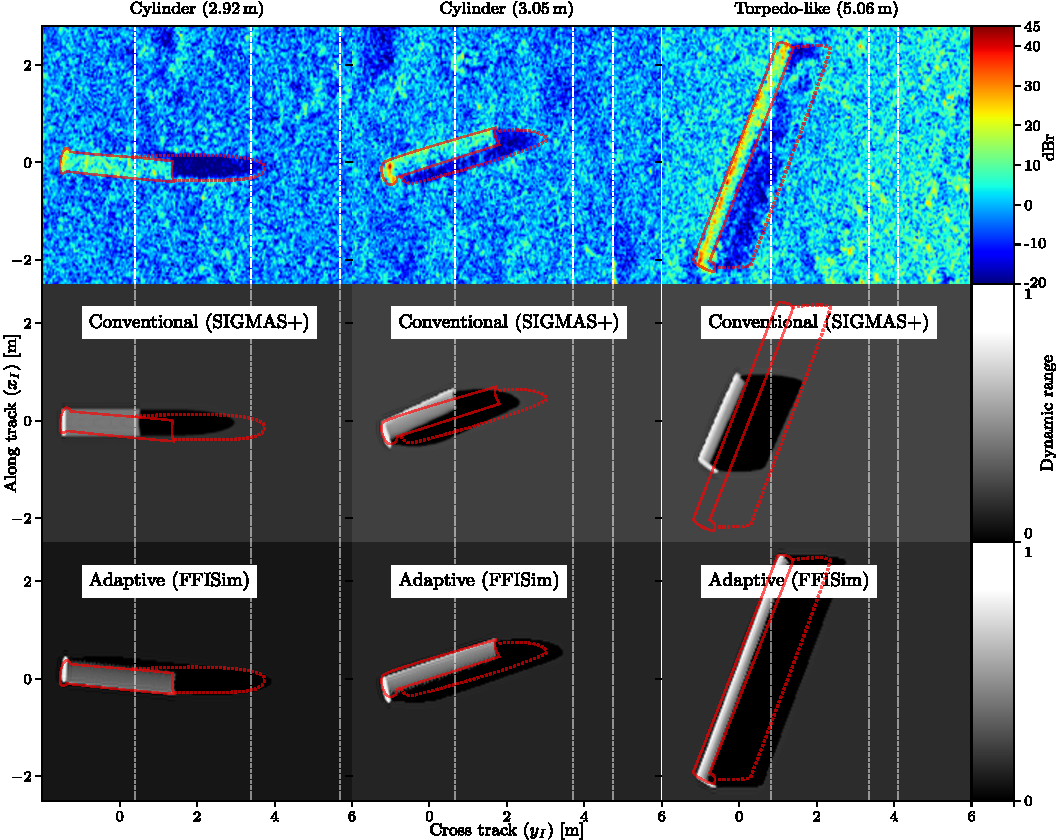
\includegraphics[width=.8\linewidth]{gfx/fig_images_sonar_simulator_tagged.pdf}%
\else%
  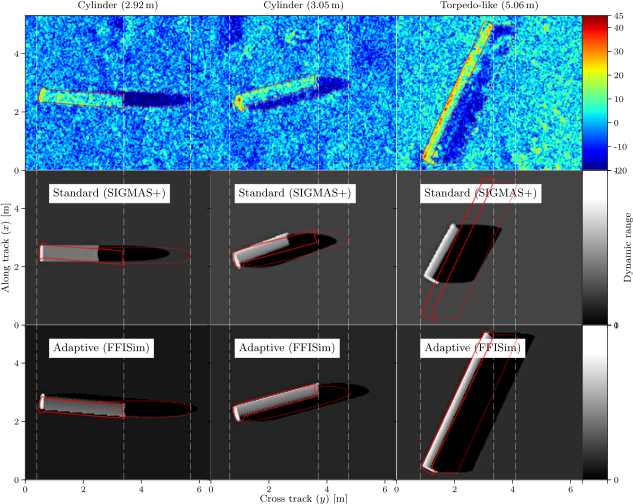
\includegraphics[width=.8\linewidth]{gfx/fig_images_sonar_simulator_tagged.svg}%
\fi
\caption{\emph{Two cylinders and a torpedo in Jesus Bay, Norway.} Top row shows isolated SAS image segment corresponding to the object, while center and bottom row show the template from the conventional and adaptive method, respectively. The contour of the SAS object is indicated with red lines. Observe that the adaptive technique perform better in the highlight, but not necessarily the shadow.}\label{IV_fig_images_sonar_simulation}%
\end{figure*}

\begin{figure*}[t]\centering%
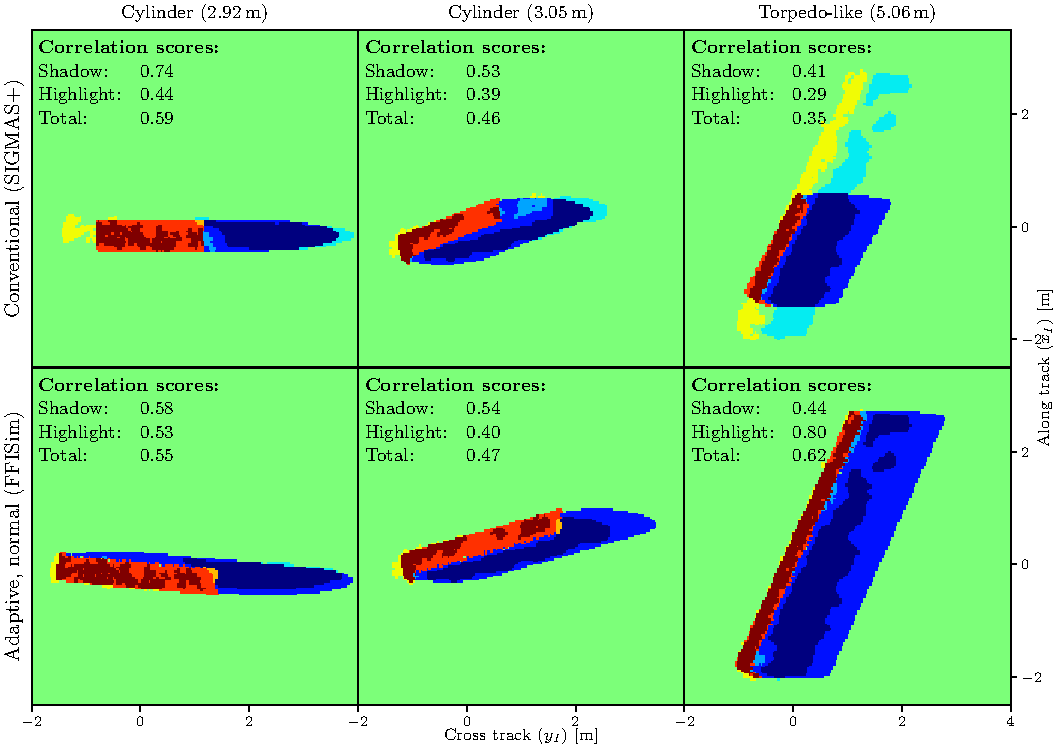
\includegraphics[width=.8\linewidth]{gfx/fig_overlay.pdf}%
% \parbox{\linewidth}{\small\centering\vspace{.5\baselineskip}
% \newline\centering\newline %\\[.5\baselineskip]
\newcommand\cdesc[2]{{\raggedright\setlength\fboxsep{0pt}
\fbox{\colorbox[HTML]{#1}{\vrule height8.5pt depth3.5pt width0pt\hspace{.5cm}}}\ \ #2\\}}
\begin{minipage}{.29\linewidth}\footnotesize
\cdesc{800000}{Template highlight and image highlight}
\cdesc{FF1000}{Template highlight only}
\cdesc{FFEB00}{Image highlight only}
\cdesc{83FF7C}{Background pixels}
\end{minipage}\mbox{}\hspace{3cm}
\begin{minipage}{.29\linewidth}\footnotesize
\cdesc{000083}{Template shadow and image shadow}
\cdesc{0014FF}{Template shadow only}
\cdesc{00EFFF}{Image shadow only}
\cdesc{00A7FF}{Template shadow and image highlight}
\end{minipage}%}
\caption{Comparison of classification performance for the standard and adaptive template technique. The three objects were more or less arbitrary picked from the scene. For the roughly 3\,m long cylinders both methods perform similarly, the standard method seemingly with a slight edge. This is no surprise given that the 3\,m long cylinder model that make up the static template database fit the actual object well here. However, for the longer torpedo-like object the adaptive technique is clearly better. This is its merit; for objects and geometries that are not included in the static template database we can expect the adaptive techniques to perform better.}\label{IV_fig_image_simulation}%
\end{figure*}

\begin{figure*}[t]\centering%
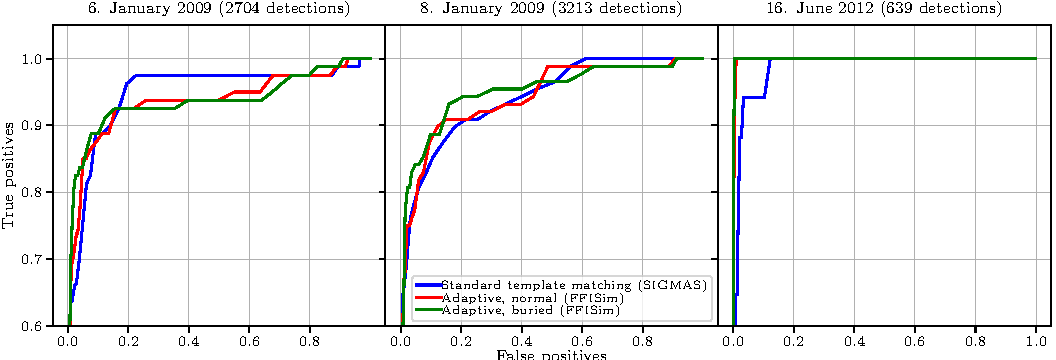
\includegraphics[width=\linewidth]{gfx/fig_rocs.pdf}%
\caption{\emph{Receiver operating characteristics (ROC) curves.} The adaptive methods }\label{IV_fig_roc_curves}%
\end{figure*}

The upcoming results will be based on experimental data from a HISAS1030 interferometric synthetic aperture sonar (SAS) attached to a HUGIN autonomous underwater vehicle (AUV), both developed by Kongsberg Maritime, Norway. The HISAS1030 is a fully digital phased array with 32 hydrophones, 100\,kHz center frequency and 30\,kHz bandwidth. It is 1.2\,m long, has a half-power beamwidth (HPBW) of 23$^\circ$, and is capable of generating SAS images with a theoretical resolution of 3-4\,cm both cross- and along-track. Our version of HUGIN also carries a camera that is used for optical inspection of interesting objects.

%To test performance of our simulator and template matching techniques where measured using experimental data from 

We present three different HUGIN runs from the Jesus Bay in Norway. The first two a couple days apart in January 2009, containing roughly 2700 and 3200 detections, respectively. The last is from June 2012 and contains roughly 650 detections. Almost all objects here are cylindric---e.g. barrels, pipe mines and torpedoes---with a length of about 3\,m.

The following three methods will be contrasted:\todo{Poor transition}
%
\begin{itemize}
\item \emph{Standard (SIGMAS+).} Picks the best template out of a set precomputed with SIGMAS+. The templates are tailored to a 3\,m long cylinder; the most frequently occurring object in the scene.
\item \emph{Adaptive, normal (FFISim).} Creates a single template with FFISim, given estimated seafloor and object orientation, and object length, width and immersion depth~\cite{Midelfart2010}. 
\item \emph{Adaptive, buried (FFISim).} Finds an "optimal" template with FFISim, given the estimated parameters described above and a search space for burial depth---modeled as rotation by $\{-4,-2,0,2,4\}^\circ$ around the cross track axis $y_\textrm{\tiny$\uvec{I}$}$.
\end{itemize}

\subsection{Processing speed}

%FFISim was designed to 
%The key selling point of FFISim is that it is very fast. 
%Note that FFISim 
%
%is used with the adaptive method due to its tighter integration with the classifier, allowing a range of templates to be generated and assessed on the GPU in a single invocation. It can produce thousands of templates per second if need be. This is why FFISim is being used in the adaptive procedure, and SIGMAS+ in the conventional procedure with a static precomputed set of templates.


Our GPU-based simulator is very fast. On a computer with a six-core Intel Core i7-3930K and a Radeon HD7970 it computes almost 1000 templates per second, each being 1 megapixel large. This makes it possible to tailor the templates very closely imaged objects. In contrast, in the standard approach a template library must be created beforehand from a limited set of parameter values. Hence, it may happen that no template in the library is a close fit of the object in the image even though the object actually is a target of interest.\todo{Rewrite paragraph}

%The edge of FFISim lies in its tighter integration with the classifier


\subsection{Classification - selected objects}


Let us first study simulation and classification performance on three typical objects from the 2012 data: Two roughly 3\,m long mines and a 5\,m long torpedo, each with unique immersion depth and aspect angle. We present the SAS image segments and templates for these objects in \Fig{IV_fig_images_sonar_simulation}, with hand-drawn red lines superimposed to mark the objects' contours. Observe the following:
%
\begin{itemize}
\item \emph{Template image quality} is similar for both SIGMAS+ and FFISim. With accurate input parameters, both simulators generate highlight and shadow regions with correct size and shape. Intensity values are also near identical (ignoring background level), as expected since they both rely on a Lambertian scattering model.
\item \emph{Template accuracy} improves when using the adaptive technique; It excels at generating accurate highlight regions, but is less convincing in shadow regions. This advantage grows the more unconventional the object is, since these objects will not be represented in the static database.
\end{itemize}

%- Template quality FFISim/SIGMAS+, similar. Same size/shape.
%- Adaptive technique for highlight, tie for shadows. Same seen in segmentation result.
%- Speed -> FFISim


%Note how the adaptive technique excels at reproducing accurate highlights, but that this does not necessarily translate into accurate shadows. 

%In terms of template quality both SIGMAS+ and FFISim produce similar results. 

%\Fig{IV_fig_image_simulation} contrasts the segmentation result of the templates with that of the SAS image---in terms of highlight, shadow and background regions. As expected the adaptive technique generally produce better matching templates, but with a surprising caveat: Improved highlight scores did not necessarily translate to better shadow scores. 


%Out of the objects in the scene we selected a 2.6\;m long cylinder that was partly buried in the sea sediments (Fig. \ref{IV_data_cylinder}). The length, immersion depth and aspect angle of this cylinder were estimated from the SAS image using our  adaptive template matching approach~\cite{Midelfart2010}. 

%Then these parameters were used by the simulator to create an adaptive template (Fig. \ref{IV_sim_cylinder}), which is an almost perfect match of the cylinder. We also created standard templates for a regular template matching approach. In this case, we assumed that the cylinder mine had a generic length of 2\;m (like a MP80 or a Murena mine) and was proud on the seafloor. Moreover, templates were created for every 10$^\text{th}$ degree of the aspect angle. We believe these assumptions to be typical for a template library for cylinder mines. 

%Note how the adaptive template obtained a much closer fit to image than the standard template. This was also reflected in the correlation scores (which were created with the method described in \cite{Midelfart2010}) that were 0.613 for the standard template and 0.813 for the adaptive template. Hence, the standard approach was less likely to classify the cylinder in the image correctly as the standard templates were not created specifically for the target.

%The main difference lies in how they integrate into the classification process: While SIGMAS+ generate one template for each invocation, FFISim can iterate through a space of parameters on the GPU before returning control to the CPU. This speeds up the template matching dramatically, allowing it to assess thousands of templates per second instead of, say, one. 

% FFISim provide templates that better match the true object orientation in this figure, but  

% Different background level. Adaptive technique excels for less normal objects/geometries.
%Overlap - Provide quantification measure. 

\subsection{Classification - all objects}

We demonstrate classification performance with receiver operating characteristic (ROC) curves in \Fig{IV_fig_roc_curves}. 

Below 20\% false positive rate (FPR) the adaptive techniques outperformed the static method in every run. This benefits e.g. mine counter measures (MCM) operations because out of 3000 detections only a few will be visually inspected up close.

Above 20\% FPR the results are less clear: The adaptive techniques performed similarly to the static method in 2012, but worse January 6. and better January 8. 2009---with 5 and 3 false detections at 20\% FPR, respectively. From visual inspection we found the cause to be a combination of fish trawler tracks and poor highlight and shadow quality.


 
%- Stm stimulated with length matching test cylinder. Perfect score against this.
%- Atm - not given to improve score. Shadow and highlight both need to match, and overfitting could lead to reduced performance.
%
%
%
%
%Good statistics drawn from the image -> adaptive better. Poor statistics -> hit and miss.
%
%
%1. Comparison with standard template library (ROC enough?)
%   ROC: Adaptive better at FPR<0.2 in all cases.
%2. Comparison with SIGMAS+
%   Fairly similar images, performance is similar. 
%   Used to create the standard template library.
%3. Comparison with search space
%   ROC: Additional search always better FPR<0.2.
%   Explain search criterion.



%SAS images - look good. Random pick objects. Lengths derived from image.


%
%1. Adaptive better? Compare with standard. Doing this in ROC
%2. Improved classification? ROCs
%3. Further improvement by doing fine-search? ROC
%
%
%An issue the adaptive technique must deal with when estimating object length 
%
%As the ROC curves indicate, the adaptive template matching techniques both  ROC curves demonstrate the 
%
%The majority of the objects in the Jesus Bay are cylinder shaped. A SAS image of three such objects are displayed in \Fig{IV_fig_image_sonar}
%
%
%
%


% \begin{figure*}[!tbp]\centering%
% \subfloat[SAS images of 2 cylinders and a torpedo.]{%
% \includegraphics[width=0.5\linewidth]{gfx/fig_images_sonar_simulation.pdf}%
% \label{IV_fig_sonar_simulation}}%
% \subfloat[Cylinder simulation with parameters estimated from SAS image: Length 2.6\;m, burial depth 0.263\;m, aspect angle 105$^\circ$.]{
% 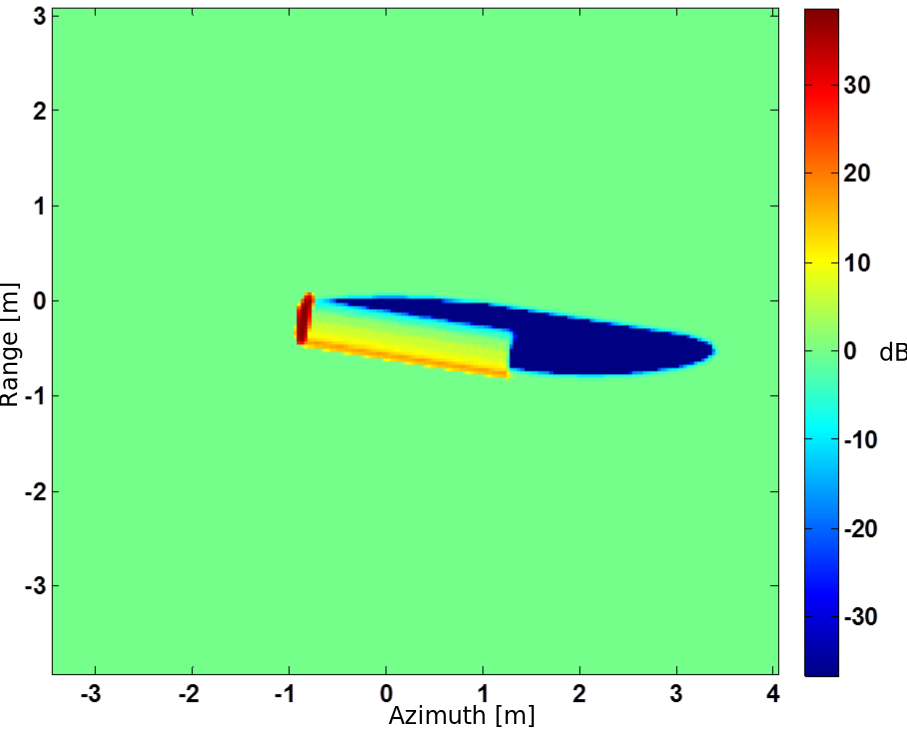
\includegraphics[drawing,width=0.5\linewidth]{gfx/sim_cylinder_submerged_adaptive.svg}%
% \label{IV_sim_cylinder}}%
% \caption{A SAS image of a cylinder and a template simulation adapted to it.}
% \end{figure*}
% 
% 
% \begin{figure*}[!tbp]\centering%
% \subfloat[SAS image of a cylinder with 2.6\;m length and 0.53\;m radius.]{%
% 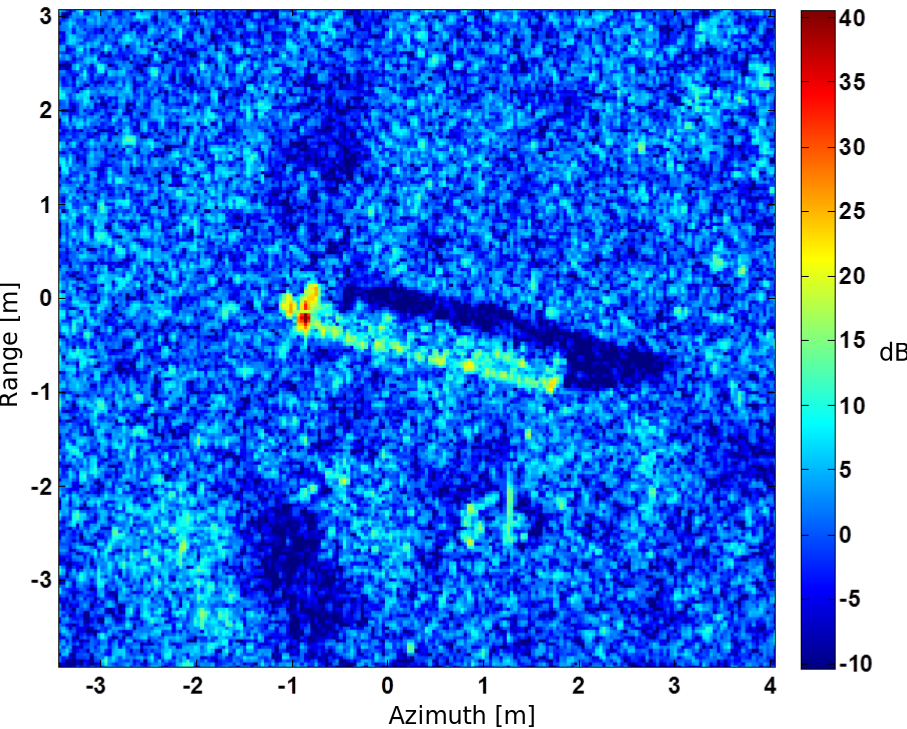
\includegraphics[drawing,width=0.5\linewidth]{gfx/data_cylinder_submerged.svg}%
% \label{IV_data_cylinder}}%
% \subfloat[Cylinder simulation with parameters estimated from SAS image: Length 2.6\;m, burial depth 0.263\;m, aspect angle 105$^\circ$.]{
% 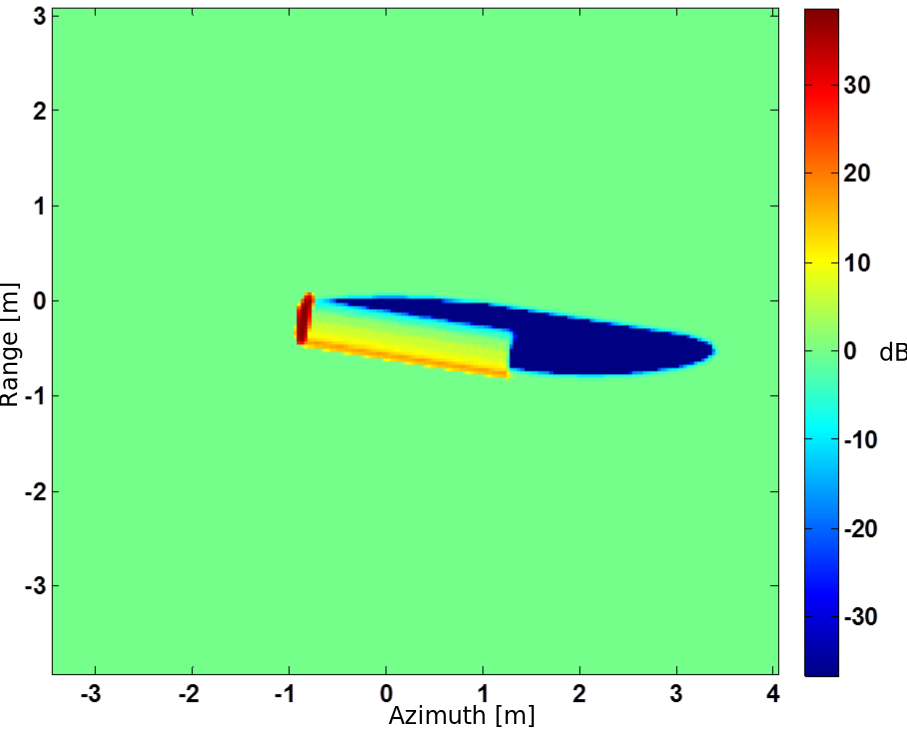
\includegraphics[drawing,width=0.5\linewidth]{gfx/sim_cylinder_submerged_adaptive.svg}%
% \label{IV_sim_cylinder}}%
% \caption{A SAS image of a cylinder and a template simulation adapted to it.}
% \end{figure*}


% \newcommand\cdesc[2]{#2}


% Whenever conventional computer graphics processing can be used to 
% GPUs are designed to provide the best possible graphics processing performance, and there large ecosystem of tools and libraries  available 
% Using a GPU to drive a simulator is advantageous since
% 
% 
% Creating a GPU-based simulator is attractive since computer is an attractive solution as there are a  graphics traits. For one over a CPU-based standard simulator is two-fold: 



%
%
%
%\begin{itemize}
%\item GPUs low power. Good for integration in AUVs.
%\item Good accuracy even with a real-time constraint in e.g. a AUV.
%\item Improved inertial navigation?
%\item Aid in understanding the key parts of the SAS image and in discovering potential flaws in the SAS image. Anomalies can be flagged to make SAS more robust?
%\end{itemize}


\section{Conclusion}\label{IV_conclusion}

One way to automatically classify objects in SAS images is to compare the imaged objects with a predefined set of templates. However, this is suboptimal as it is infeasible to create accurate templates for all the relevant configurations of seabeds and objects. To solve this we have implemented a SAS simulator that creates the templates in delayed real-time based on parameters estimated from the current scene. In our studies this improves the match between the SAS objects and their corresponding template significantly in most cases.

To obtain the delayed real-time performance we implemented the simulator on a GPU. These devices have a theoretical peak performance that is typically an order of magnitude higher than CPUs in a comparable price range. We found this potential to be effectively utilized with the well matured and highly optimized OpenGL graphics processing API. Our simulator use this framework for most of the scene processing.

A final post-processing step is performed in OpenCL, which allow general purpose GPU programming. It interoperates well with OpenGL and adds a lot of flexibility to the simulation process. This is valuable as the simulator is still being actively developed and will likely see new features that can not be easily implemented in OpenGL alone.

With good image quality or low FRP, or both, the adaptive methods did better. However, when this was not the case, it was less clear who the winner was. The standard method of using a static template library generally did well here, . 

In terms of template quality both SIGMAS+ and FFISim are similar. The main difference lies in how they integrate into the classification process: While SIGMAS+ generate one template for each invocation, FFISim can iterate through a space of parameters on the GPU before returning control to the CPU. This speeds up the template matching dramatically, allowing it to assess thousands of templates per second instead of, say, one. 
 
%
%\begin{itemize}
%\item Motion compensation
%\item 
%\end{itemize}

\ifPhdDoc
\clearpage
\appendix
\renewcommand\thesection{\Roman{section}}
\else
\appendices
\fi

\section{Active rotations and transforms}\label{IV_active_rotations_transforms} 

The geometrical intent of an active rotation is to move a point. With our notation this can be expressed as either
%
\begin{align}
\m{CL}
\vec{p}_{M\g{Vtot}{V}_{\color{Green}\!\textrm{new}}}
= \vec{R} \; \vec{p}_{M\g{V2}{V}}\m{CR}
\quad\text{or}\quad
\m{CL2}
\dvec{p}_{M\g{Vtot2}{V}_{\color{Green}\!\textrm{new}}}^M
= \mat{R}^M \dvec{p}_{M\g{V4}{V}}^M,\m{CR2}
\label{IV_eq_active_rotation}
 \\\nonumber
 %\qquad\qquad
%
%\\[.5\baselineskip]\nonumber % Adjust spacing as necessary
\tikz[overlay,remember picture]{
  % Set up some general bounding box markers
  \coordinate(CC) at      ($ .5*(CL)       + .5*(CR)                         $);
  \coordinate(CC2) at     ($ .5*(CL2)      + .5*(CR2)                        $);
  \coordinate(_MV) at     ($ (V2.south)    + (-\baselineskip,-\baselineskip) $);
  \coordinate(_MVtot) at  ($ (Vtot.south)  + ( \baselineskip,-\baselineskip) $);
  \coordinate(_MV2) at    ($ (V4.south)    + (-\baselineskip,-\baselineskip) $);
  \coordinate(_MVtot2) at ($ (Vtot2.south) + ( \baselineskip,-\baselineskip) $);
  % Draw arrows and text
    \draw[]                    ($ (V2.south)    - (0em,\tpad) $)
            to[out=-90, in=0]     (_MV)
            to[out=180, in=0]     (_MVtot)
            to[out=180, in=-90]($ (Vtot.south)  - (0em,\tpad) $);
    \draw[]                    ($ (V4.south)    - (0em,\tpad) $) 
            to[out=-90, in=0]     (_MV2)
            to[out=180, in=0]     (_MVtot2)
            to[out=180, in=-90]($ (Vtot2.south) - (0em,\tpad) $);
}
\end{align}
%
%\begin{align}
%\vec{R}&\colon \mathbb{V} \to \mathbb{V} \\
%\vec{R}_{IM}&\colon \uvec{I} \to \uvec{M} \subset \vec{R} \\
%\dvec{R}&\colon \mathbb{R}^N \to \mathbb{R}^N \\
%\dvec{R}_{IM}&\colon \uvec{I} \to \uvec{M} \subset \dvec{R} \\
%\label{IV_eq_active_rotation}
%\end{align}
%
% Implicit representation: (x,y,z) subject to x²+y²+z²=c -> no 
depending on whether the free or decomposed form is sought, respectively, and where $\vec{R}\colon \mathbb{V}^N \to \mathbb{V}^N$ and $\dvec{R}^M\colon \mathbb{R}^N \to \mathbb{R}^N$. Beware that the rotation matrix can be identical---both notationally and numerically---in the active and passive case, say, if $\dvec{R}^M$ was replaced by $\dvec{R}_{IM}$ in \eq{IV_eq_active_rotation}. Thus, the geometrical intent must be inferred from the position vector notation; Either the point changes, or the representation does, but never both.




\section{Transformation matrices}\label{IV_transformation_matrices} 

and their orientations by a rotation dyadic $\vec{R}_{IM}$ mapping any vector in $\uvec{M}$ to $\uvec{I}$ (which includes the basis vectors),
%
\begin{align}
\vec{R}_{IM}\colon \uvec{M} &\to \uvec{I}\label{eq_rotation_dyadic}\\
\vec{M}_i &\mapsto \vec{I}_i \quad \forall i. \nonumber
\end{align}

We define $\vec{R}_{AB}$ as a rotation---from $\uvec{A}$ to $\uvec{B}$---by angle $\theta\in\mathbb{R}$ clockwise around unit vector $\hat{r}\in\mathbb{V}$ in $\mathbb{R}^3$ Euclidean space using Euler-Rodrigues' formula,

\subsection{Free Euler-Rodrigues}\label{IV_sec:free_euler_rodrigues}
%
\begin{align}\label{eq:M}
%\uvec{A} = \vec{R}_{\uvec{A}\uvec{B}}\uvec{B} \\
\vec{R}_{AB}
&\triangleq %e^{j\overset{\times}{r}\theta}=\nn
 \vec{I} + \overset{\times}{r}\sin\theta + \overset{\times}{r}{}^2(1-\cos\theta) \in SO(3),
\end{align}
%
where $\vec{I}$ is the identity, and $\overset{\times}{r}$ is the skew-symmetric (or cross-product) matrix of $\hat{r}$,
%
\begin{align}
\overset{\times}{r}
&\triangleq \bmat{\hat{r}\times} \triangleq \bmat{
0 & -\hat{r}_z & \hat{r}_y \\
\hat{r}_z & 0 & -\hat{r}_x \\
-\hat{r}_y & \hat{r}_x & 0
},
\end{align}
%
and the angle $\theta$ and rotation axis $\hat{r}_{AB}$ can be expressed in terms of $\vec{p}_A$ and $\vec{p}_{B}$,
%
\begin{align}
\theta
&= \mathrm{acos}\frac{\vec{p}_{A}\cdot\vec{p}_{B}}{\lVert\vec{p}_{A}\rVert\lVert\vec{p}_{B}\rVert} \\
\hat{r}_{AB} &=  \frac{\vec{p}_{A}\times\vec{p}_{B}}{\lVert\vec{p}_{A}\rVert\lVert\vec{p}_{B}\rVert}
\end{align}
%
where $\cdot$ and $\times$ denotes the dot- and cross-product, respectively.\todo{Mighty long and heavy sentence... Yikes}

$SO(3)$ refers to special (\emph{i.e.} right handed) orthogonal $\mathbb{R}^{3\times3}$ matrices, where the handedness is verified by determinant $\big|R\big|=1$ (as opposed to $\pm1$), and the orthogonality follows from the skew symmetry of $\overset{\times}{r}_{AB}$. $SO(3)$ are also known as rigid transformations, because they preserve the distance and orientation between points~\cite{Murray1994}\footnote{Pages 26-27}\todo{Valid page specification?}.

{\color{blue}Below is the old text}

We restrict our attention to linear transforms of the kind $\mat{L}_{AB} = \mat{R}_{AB}\;\mat{S}_{AB}$ where the former is a rotation matrix and the latter a scaling matrix. The rotations are performed with Euler-Rodrigues formula~\cite{Dai2015} using a unit length rotation axis $\dvec{\hat{r}}_{AB}^A$ and angle $\theta_{AB}$:
%
\begin{align}\label{eq:M}
\mat{R}_{AB} &= \I + \sin\theta_{AB}\;[\dvec{\hat{r}}^A\times] + (1-\cos\theta_{AB})\;[\dvec{\hat{r}}^A\times]^2 \in\mathbb{R}^{3\times3}
\end{align}
%
where $\big[\dvec{\hat{r}}_{AB}^A\big]$ is the open-right cross product matrix of $\dvec{\hat{r}}^A$ and $\mat{I}$ is the identity matrix. 

% %\dvec{\hat{p}}_{A\times{}B}^C
\begin{align}
\theta_{AB}
&= \mathrm{acos}\frac{\dvec{p}_{A}^{C}\cdot\dvec{p}_{B}^{C}}{\lVert\dvec{p}_{A}^{C}\rVert\lVert\dvec{p}_{A}^{C}\rVert} \\
\dvec{\hat{r}}_{AB}^C &=  \frac{\dvec{p}_{A}^{C}\times\dvec{p}_{B}^{C}}{\lVert\dvec{p}_{A}^{C}\rVert\lVert\dvec{p}_{A}^{C}\rVert}
\end{align}

% http://lairs.eng.buffalo.edu/pdffiles/pconf/C10.pdf
% http://www.navlab.net/Publications/Inertial_Navigation_-_Theory_and_Applications.pdf

Each data model that we load into OpenGL is defined in its own local coordinate system. To map them into OpenGL world coordinates a set of common transformation matrices are applied to each model's vertices:
%
\begin{align}
\bmat{x_t \\ y_t \\ z_t \\ w}_\text{\parbox{1cm}{\setlength\baselineskip{0.3cm}transformed\\model}} &= \boldsymbol{T} \cdot \boldsymbol{R} \cdot \boldsymbol{S} \cdot \bmat{x \\ y \\ z \\ w}_\text{model}.
\end{align}
%
Here a model vertex at position $(x,y,z)$ is first scaled with $\boldsymbol{S}$, then rotated with $\boldsymbol{R}$ and finally translated with $\boldsymbol{T}$, resulting in the transformed coordinates $(x_t,y_t,z_t)$. The parameter $w$ defines whether the vertex is a position ($w=1$) or a direction ($w=0$), which need to be handled differently. While these matrices are well-known in the field of computer graphics, there exist several different conventions but we supply them here for completeness.

%Adding some phantom space to align the columns of the next matrices
\newcommand\pc[1]{\phantom{ml}#1\phantom{ml}}
The scaling and translation matrices are simple:
%
\begin{align}
\boldsymbol{S}(\s) &= \bmat{
   s_x  &  0   & 0  & 0 \\
   0    &  s_y  &  0    &  0 \\
   0    &  0    &  s_z  &  0 \\
   \pc{0}    &  \pc{0}    &  \pc{0}    & \pc{1} \\
  },
  \end{align}
%
and
%
\begin{align}
\boldsymbol{T(\vec\Delta}) &= \bmat{
	1  &  0  &  0  &  \Delta_x \\
	0  &  1  &  0  &  \Delta_y \\
	0  &  0  &  1  &  \Delta_z \\
 \pc{0}  &   \pc{0}  &   \pc{0}  &   \pc{1} \\
},
\end{align}
%
where $\s = (s_x, s_y, s_z)$ and $\vec\Delta = (\Delta_x, \Delta_y, \Delta_z)$ are the scaling and translation factors.

Rotations will be specified using yaw ($\phi$), pitch ($\theta$) and roll ($\psi$), representing clockwise rotations around the intrinsic $z$-, $y$- and $x$-axis, respectively. Rotation order follow the intrinsic Tait-Brian $Z$-$Y'$-$X''$ convention, in which roll is applied first, then pitch and finally yaw:
%
\begin{align}
\R(\phi_x) = \R_z(\phi)\R_y(\theta)\R_x(\psi),
\end{align}
%
where
%
\begin{align}
\R_x(\psi) &= \bmat{
    1  &   0        &  0         &  0 \\
    0  &  \cos\psi  &  -\sin\psi &  0 \\
    0  &  \sin\psi  &  \cos\psi  &  0 \\
\pc{0} &  \pc{0}    &  \pc{0}    &  \pc{1} \\
}, \\[.5\baselineskip]
\R_y(\theta) & = \bmat{
\cos\theta	& 0          & \sin\theta & 0 \\
0				& 1          & 0          & 0  \\
-\sin\theta & 0          & \cos\theta & 0  \\
\pc{0}      &  \pc{0}    & \pc{0}     & \pc{1} \\
},
%\\[0\baselineskip]
\intertext{and}
%\\[0\baselineskip]
\R_z(\phi) &= \bmat{
\cos\phi	&  -\sin\phi   &  0      &  0 \\
\sin\phi	&  \cos\phi    &  0      &  0 \\
0			&  0           &  1      &  0 \\
\pc{0}	&  \pc{0}      &  \pc{0} &  \pc{1} \\
}.
\end{align}
%
Note that at $\theta=\frac{\pi}{2}$ we have $\phi=-\psi$, and at $\theta=-\frac{\pi}{2}$ we have $\phi=\psi$. This effect, in which one degree of freedom is lost, is known as Gimbal lock. Any three-parameter specification of an orientation in three-dimensional space has this problem. Adding a fourth parameter can resolve the issue. e.g. by direct specification of orientation in terms of a rotation axis and angle. This can be achieved using the Euler-Rodrigues formula or with quaternions. The latter has the added benefit of reduced computational complexity, improved numerical stability and simple ways to perform spherical interpolations. An alternative used extensively at FFI that is non-singular and practical is the $\vec n$-vector notation~\cite{Gade2010}. However, we stick with the Euler-angle representation here due to their simplicity.


%xyz - system space coordinates (fixed unmoving)
%XYZ - system body coordinates (body fixed moving)


Translation is performed last. 

%and the bases in terms of a linear operator $\vec{R}_{AB} \in SO(3)$ which rotates about an axis $\hat{r}$ by angle $\theta$,
%%
%\begin{align}\label{eq:M}
%\vec{R}_{AB}
%&=
%% \vec{I} + \overset{\times}{r}\sin\theta + \overset{\times}{r}{}^2(1-\cos\theta).
%\vec{I} + \sin\theta(\hat{r}\times) + (1-\cos\theta)(\hat{r}\times)^2.
%\end{align}
%%
%where $\times$ is the cross-product. $\hat{r}$ and $\theta$ relates to $\uvec{A}$ and $\uvec{B}$ by
%%
%\begin{align}
%\hat{r} = \frac{\uvec{A}\times\uvec{B}}{\lVert\uvec{A}\rVert\lVert\uvec{B}\rVert}
%\quad\mathrm{and}\quad
%\theta  = \mathrm{acos}\frac{\uvec{A}\cdot\uvec{B}}{\lVert\uvec{A}\rVert\lVert\uvec{B}\rVert},
%\end{align}
%%
%where $\times$ and $\cdot$ signifies the cross- and dot-product, respectively.
%
%and the angle $\theta$ and rotation axis $\hat{r}_{AB}$ can be expressed in terms of $\vec{p}_A$ and $\vec{p}_{B}$,
%%
%\begin{align}
%\theta
%&= \mathrm{acos}\frac{\vec{p}_{A}\cdot\vec{p}_{B}}{\lVert\vec{p}_{A}\rVert\lVert\vec{p}_{B}\rVert} \\
%\hat{r}_{AB} &=  \frac{\vec{p}_{A}\times\vec{p}_{B}}{\lVert\vec{p}_{A}\rVert\lVert\vec{p}_{B}\rVert}
%\end{align}
%\begin{align}
%\theta
%&= \mathrm{acos}\frac{\vec{p}_{A}\cdot\vec{p}_{B}}{\lVert\vec{p}_{A}\rVert\lVert\vec{p}_{B}\rVert} \\
%\hat{r}_{AB} &=  \frac{\vec{p}_{A}\times\vec{p}_{B}}{\lVert\vec{p}_{A}\rVert\lVert\vec{p}_{B}\rVert}
%\end{align}
%%
%The position vector $\vec{p}_{\udot{A}\udot{B}}$ go from $\udot{A}$ to $\udot{B}$ only depends on these points. Similarly, the matrix $\vec{R}_{\uvec{A}\uvec{B}}$ only depends on vectors; $\vec{R}_{\uvec{A}\uvec{B}}\uvec{B}$ rotates $\uvec{B}$ to $\uvec{B}$, $\uvec{A}\vec{R}_{\uvec{A}\uvec{B}}$ rotates $\uvec{A}$ to $\uvec{B}$. 
%


% use section* for acknowledgement
\ifCLASSOPTIONcompsoc% % This command fixes abstract positioning for compsoc articles:
% \IEEEdisplaynotcompsoctitleabstractindextext
% 
% % (Optional) Add some extra info on cover page of peer review papers:
% % \ifCLASSOPTIONpeerreview
% % \begin{center} \bfseries EDICS Category: 3-BBND \end{center}
% % \fi
% 
% % Insert page break and insert second title (peer review mode)
% \IEEEpeerreviewmaketitle
% 
% 
% 
  \section*{Acknowledgments}
\else
  \section*{Acknowledgment}
\fi


The authors would like to express their gratitude to the Norwegian Defence Research Establishment (FFI) for funding the development of the simulator.

% Can use something like this to put references on a page
% by themselves when using endfloat and the captionsoff option.
\ifCLASSOPTIONcaptionsoff
  \newpage
\fi

\ifPhdDoc
%   \printbibliography[title=References,heading=subbibliography]
%    \bibliographysty
%    \bibliography{library.bib}
%    \print
\else
   \ifBuildBibliography
      \typeout{===Mybib===}
      \bibliographystyle{IEEEtran}
      \bibliography{references}

   \else
      \typeout{===MyStaticbib===}
      % Paste here
   \fi

  
   % Generated by IEEEtran.bst, version: 1.13 (2008/09/30)
   % \begin{thebibliography}{10}
   % stuff here
   % \end{thebibliography}
   
   
   
\begin{IEEEbiography}[{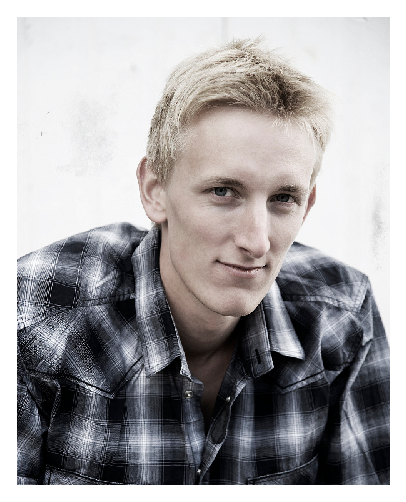
\includegraphics[width=1in,height=1.25in,clip,keepaspectratio]{bio/jo_inge.eps}}]{Jo Inge Buskenes}
received the B.Sc. degree in electrical engineering from Gj\o{}vik College University, Norway, in 2007, and the M.Sc. degree in instrumentation for particle physics from the University of Oslo, Norway, in 2010. He is currently pursuing the Ph.D. degree in acoustic image reconstruction and high performance computing at the University of Oslo.

His industry experience includes development of digital electronics at the European Organization for Nuclear Research (CERN), Geneva, Switzerland (2007-2008). He has lectured in digital signal processing at the Gj\o{}vik College University (2009), and at the University of Oslo (2010-2013). Current affiliation is with The Norwegian Defence Research Establishment, Kjeller, Norway, for which he is developing radar systems (2015-), and formerly sonar systems (2009, 2013).

His research interests include radar and sonar technology, aptive image reconstruction, high performance computing, intelligent detector design and open source software.
\end{IEEEbiography}
   % 
\begin{IEEEbiography}[{\includegraphics[width=1in,height=1.25in,clip,keepaspectratio]{bio/jon_petter.eps}}]{Jon Petter \AA{}sen}
(S'12) was born in Porsgrunn, Norway in 1986. He received the B.Sc. and M.Sc. degree in computer science from the University of Oslo, Norway, in 2010. He is currently pursuing his Ph.D. degree in medical ultrasound technology at the Norwegian University of Science and Technology (NTNU) Medical Imaging Lab (MI-Lab), Trondheim, Norway. His research interests include adaptive ultrasound processing techniques and acceleration of ultrasound algorithms using Graphics Processing Units (GPUs). 
\end{IEEEbiography}
   % 
\begin{IEEEbiography}[{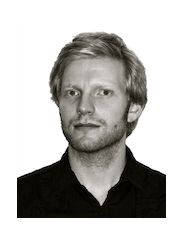
\includegraphics[width=1in,height=1.25in,clip,keepaspectratio]{bio/carl-inge.eps}}]{Carl-Inge Colombo Nilsen}
(S'06-M'10) received the M.Sc. and Ph.d. degrees in computer science from the University of Oslo, Norway, in 2005 and 2010. He is currently working at the University of Oslo as a postdoctoral research fellow. His research interests include signal and array processing for ultrasound imaging and other acoustical applications.
\end{IEEEbiography}
   % 
\begin{IEEEbiography}[{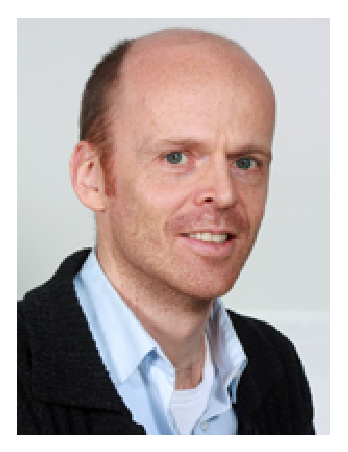
\includegraphics[width=1in,height=1.25in,clip,keepaspectratio]{bio/andreas.eps}}]{Andreas Austeng}
was born in Oslo, Norway, in 1970. He received the M.Sc. degree in physics in 1996 and the Ph.D. degree in computer science in 2001, both from the University of Oslo. Since 2001, he has been working at the Department of Informatics, University of Oslo, first as a postdoctoral research fellow and currently as an associate professor. His research interests include signal and array processing for acoustical imaging.
\end{IEEEbiography}
   
   
   % 
   % IMAGE METRICS
   %
   % - Point spread function (res via main lobe width, SAS gain via PDF height)
   % - Constrast measures
   %
   % ACR = cL/2
   % C = (s+n)/n ratio
   % - 
   % WHO's needing processing power
   % - Centre for Maritime Research and Experimentation
   
   
   \vfill 
   
   
\newpage

\section{Wave Equation}

The wave equation describes how a wave moves as a function of both time and space. It forms the basis for all mathematical modeling of waves, so we will spend some time to derive it here. We will treat acoustical waves since they are most relevant to the topic in this thesis, but we could have derived it from electromagnetic waves using Maxwell's equations with some boundary conditions.

\begin{figure}[ht]
\begin{floatrow}

\floatbox{figure}[\linewidth][\FBheight][t]{%
\caption{Mass flow}}{%
\graphicsAI[drawing,width=.77\linewidth]{gfx/wave_equation_mass_flow.svg}}%

\floatbox{table}[\linewidth][\FBheight][t]{%
\caption{Symbol description}}{%
\begin{tabular}[c]{c c l}\hline
\rowcolor{tabBlue}\bf Symbol & \bf Unit & \bf Description \\\hline
$s$ & Pa = N/m$^2$ & Pressure \\
$\rho$ & kg/m$^3$ & Density \\
$S$ & Nm/K & Entropy \\
$\vec v$ & m/s & Mass velocity \\
$\dot{\boldsymbol{m}}$ & kg/s & Mass flow
\end{tabular}}

\end{floatrow}
\end{figure}


We begin by defining the net \textbf{mass flow} through a volumetric element $dV = dx\,dy\,dz$:
%
\begin{align}
\frac{\dot{\boldsymbol{m}}_\text{net}}{dV} = \ux\frac{\partial \rho\,\v}{\partial x} + \uy\frac{\partial \rho\,\v}{\partial y} + \uz\frac{\partial \rho\,\v}{\partial z} = \nabla \cdot (\rho\v).
\end{align}
%
The space and time dependence of the mass density $\rho = \rho(\p,t)$ and particle velocity $\v = \v(\p,t)$ is omitted here and in the following text for brevity. If the volume of the element is fixed a change in mass must equal a corresponding change in density. This is the law of \textbf{mass conservation}:
%
\begin{align}
\frac{\partial\rho}{\partial t} = -\nabla \cdot (\rho\v). \label{wave_eq_mass_conservation}
\end{align}
%
An additional constraint we may surely apply is the Euler's equation, a modification of Newton's second law the the total acceleration $a$ is is a function of both time and space:
%
\begin{align}
\frac{F}{dV} = \frac{m}{dV} a = \rho\Big(\frac{\partial\v}{\partial t} + \v\cdot\nabla\v\Big) = -\nabla s. \label{wave_eq_euler}
\end{align}
%
Next, an \textbf{equation of state} is needed to relate a change in density to a change in pressure. We assume our volume element to be isentropic, i.e. that the entropy is constant, or equivalently that total energy of the system is proportional to its temperature. This is true for any system that is reversible and adiabatic, i.e. that when no transfer of matter or heat occurs between the system and its surroundings. The pressure of the system then just depends on the mass density:
%
\begin{align}
s = s(\rho) \label{wave_eq_sound_pressure}
\end{align}

With this we have assumed the system to be \emph{loss-less}. In reality a passing sound wave will heat the fluid and add to the entropy, causing additional attenuation of the wave, but we will not be concerned with attenuation in this thesis.

\subsection{Linearization}

Equation (\ref{wave_eq_mass_conservation}), (\ref{wave_eq_euler}) and (\ref{wave_eq_sound_pressure}) are non-linear, but can be linearized by assuming each quantity to be a steady-state, time-independent value plus a fluctuation term:
%
\begin{align}
s = s_0 + s'  \qquad\qquad \rho = \rho_0 + \rho' \qquad\qquad \v = \v_0 + \v'
\end{align}
%
Taylor expanding (\ref{wave_eq_sound_pressure}) around zero yields:
%
\begin{align}
s(\rho) = s_0 + \frac{\partial s}{\partial\rho}(\rho-\rho_0) + \frac{1}{2}\frac{\partial^2 s}{\partial\rho^2}(\rho-\rho_0)^2 + \dots\label{wave_eq_sound_taylor_full}
\end{align}
%
Assuming a linear relationship between changes in pressure and volume the pressure perturbation term is simply:
%
\begin{align}
s' = \frac{\partial s}{\partial\rho}(\rho-\rho_0) = \frac{\partial s}{\partial\rho}\rho' = c^2\rho'. \label{wave_eq_sound_taylor_first}
\end{align}
%
When treating the Euler equation the same way we obtain:
%
\begin{align}
-\nabla (s_0 + s') &= (\rho_0 + \rho') \Big(\frac{\partial(\v_0 + \v')}{\partial t} + (\v_0 + \v')\cdot\nabla(\v_0 + \v')\Big) \nn
-\nabla s' &= (\rho_0 + \rho') \Big(\frac{\partial\v'}{\partial t} + \v'\cdot\nabla\v'\Big) \nn
\end{align}
%
When acceleration mainly depends on time, and the pressure fluctuations are relatively small,
%
\begin{align}
\frac{\partial\v'}{\partial t} >> \v'\cdot\nabla\v' \qquad\qquad\text{and}\qquad\qquad \rho_0 >> \rho',
\end{align}
%
then
%
\begin{align}
-\nabla s' &= \rho_0 \frac{\partial\v'}{\partial t}.
\end{align}
%
Finally, for the mass conservation we have:
%
\begin{align}
\frac{\partial(\rho_0 + \rho')}{\partial t} &= -\nabla \cdot \big((\rho_0 + \rho')(\v_0 + \v')\big)\nn
\frac{\partial\rho'}{\partial t} &= -\rho_0\nabla \cdot \v'. \label{wave_eq_mass_conservation2}
\end{align}
%
This assumes that the density is constant inside the volume element.

\begin{align}
\nabla\cdot(-\nabla s') &= \nabla\cdot\Big(\rho_0 \frac{\partial\v'}{\partial t}\Big) &
\frac{\partial}{\partial t}\frac{\partial\rho'}{\partial t} &= \frac{\partial}{\partial t}\Big(-\rho_0\nabla \cdot \v'\Big)\nn
-\nabla^2 s' &= \rho_0 \nabla\cdot\frac{\partial\v'}{\partial t} &
\frac{\partial^2\rho'}{\partial t^2} &= \frac{1}{c^2}\frac{\partial^2 s}{\partial t^2} = -\rho_0\nabla\cdot\frac{\partial \v'}{\partial t}
\end{align}
%
and we can now see that
%
\begin{align}
\nabla^2 s' - \frac{1}{c^2}\frac{\partial^2 s'}{\partial t^2} = 0.
\end{align}
%
This is called the homogeneous lossless wave equation, because there is no source term. The inhomogeneous equation can be obtained in a similar way, by altering the linearized continuity equation to:
%
\begin{align}
\frac{\partial\rho'}{\partial t} &= -\rho_0\nabla \cdot \v' - \rho_0f(\p,t). \label{wave_eq_mass_conservation_source}
\end{align}
%
where $\rho_0f(\p,t)$ is the rate of mass change (in $\left[\frac{\text{kg}}{\text{m}^3\text{s}}\right]$) caused by the source. Following the exact same procedure as before we obtain:
%
\begin{align}
\nabla^2 s' - \frac{1}{c^2}\frac{\partial^2 s'}{\partial t^2} = \rho_0\frac{\partial f(\p,t)}{\partial t}.
\end{align}
%

\section{Solution}

Instead of solving the wave equation directly, we will make a qualified guess that the solution takes the form of a complex exponential in both time and space. For rectangular coordinates this can be written as:
%
\begin{align}
s(\p,t) &= A\,e^{j(\omega t - \k\cdot\p)}
\end{align}
%
Inserting this into the wave equation yields:
%
\begin{align}
\nabla^2 s = \frac{\partial^2 s}{\partial x^2} + \frac{\partial^2 s}{\partial y^2} + \frac{\partial^2 s}{\partial z^2} &= \frac{1}{c^2}\frac{\partial^2 s}{\partial t^2} \nn
(-jk_x)^2 s + (-jk_y)^2 s + (-jk_z)^2 s &= \frac{(-j\omega)^2}{c^2} s \nn
k_x^2 + k_y^2 + k_z^2 &= |\k|^2 = \frac{\omega^2}{c^2} \\
|\k| &= \frac{\omega}{c}
\end{align}
%
Hence, whenever we can assume the spatial and temporal frequency to be related directly by the sound speed, $|\k| = \frac{\omega}{c}$, then this assuming a complex exponential should be fair.

\section{Absorption}

Our derivation of the wave equation assumed no loss of energy. In practice the wave's energy is abosorbed through viscous losses, heat conduction losses and intermolecular losses. These are strongly dependent on frequency. The wave equation can be adapted to account for absorption by assuming a complex sound speed, which will lead to a solution to the wave equation with a real exponential term. In this thesis we will not concern ourselves 

\section{Roughness}

For a plane monochromatic wave the Rayleigh roughness parameter is quantified by:
\begin{align}
\Delta\varphi = 2k\xi\cos\theta.
\end{align}
Here $\theta$ is the incidence angle, $k = \frac{2\pi}{\lambda}$ is the wavenumber of the incoming wave, $\xi$ is the distance from the scattering point to the mean surface plane, and $\Delta\varphi$ is the phase difference.

\begin{figure}[th]
\graphicsAI[drawing,width=\linewidth]{gfx/roughness.svg}
\end{figure}

To see how roughness affects the specular reflection we compute the mean reflected wave as
\begin{align}
<p> &= V\int\limits_{-\infty}^{\infty} e^{-j\Delta\varphi(\xi)} p(\xi) d\xi,
\end{align}
where $p(\xi)$ is the probability density function of $\xi$. If we assume normal distribution, we get:
\begin{align}
<p> &= V\int\limits_{-\infty}^{\infty} e^{-j2k\xi\cos\theta} \frac{1}{\sqrt{2\pi}\sigma}e^{-\frac{\xi^2}{2\sigma^2}} d\xi \nn
&= \frac{V}{\sqrt{2\pi}\sigma} \int\limits_{-\infty}^{\infty} e^{-\frac{\xi^2}{2\sigma^2}-j2k\xi\cos\theta} d\xi &\Big|{\begin{matrix}\scriptscriptstyle\hspace{-0.64cm} a = \frac{1}{2\sigma^2}\\
\scriptscriptstyle b = -j2k\cos\theta\end{matrix}}\nn
&= A \int\limits_{-\infty}^{\infty} e^{-a\xi^2 + b\xi} d\xi \nn
&= A \int\limits_{-\infty}^{\infty} e^{-a(\xi - \frac{b}{2a})^2 - \frac{b^2}{4a}} d\xi \nn
&= A e^{\frac{-b^2}{4a}} \int\limits_{-\infty}^{\infty} e^{-a(\xi - \frac{b}{2a})^2} d\xi & \Big|_{y = \xi - \frac{b}{2a}}\nn
&= A e^{\frac{-b^2}{4a}} \int\limits_{-\infty}^{\infty} e^{-ay^2} dy & \Big|_{z = \sqrt{a} y}\nn
&= A e^{\frac{-b^2}{4a}}\frac{1}{\sqrt{a}} \int\limits_{-\infty}^{\infty} e^{-z^2} dz \nn
&= A e^{\frac{-b^2}{4a}}\sqrt{\frac{\pi}{a}} \nn
&= \frac{V}{\sqrt{2\pi}\sigma} \sqrt{\frac{\pi}{\frac{1}{2\sigma^2}}} e^{\frac{-(-j2k\cos\theta)^2}{4\frac{1}{2\sigma^2}}} \nn
&= V e^{-2k^2\sigma^2\cos^2\theta}
\end{align}
This reflection coefficient is valid when the Rayleigh parameter is small (i.e. small frequency and relief amplitude), and at grazing incidence. Conventional limit of validity is $\frac{\pi}{2}$, which corresponds to $\sigma = \frac{\lambda}{8\cos\theta}$ and a coherent loss of 10.7dB.



\section{LCA tricks}

Let $\x$ be the data received by an array, pre-steered to some pixel in the image, and $\w$ be the window applied to these spatial data. Then we defined the beamformer outout $z$ as the weighted sum of the data:
%
\begin{align}
z(\w,\x) = \w\H\x = \sumb{m=0}{M-1} w_m x_m^*
\end{align}
%
Now let us choose a trigonometric window function:
%
\begin{align}
\w = \frac{e^{j\varphi}}{2\pi\alpha}\big(\alpha + (1-\alpha)\cos\left(\frac{2\pi n}{N-1}\right)\big)
\end{align}
%
Inserting this yields:
%
\begin{align}
\w\H\x &= \sumb{m=0}{M-1} e^{j\varphi}\Big(\alpha + (1-\alpha)\cos\theta\Big) x_m^* \nn
&= \sumb{m=0}{M-1} e^{j\varphi}\Big(\alpha + (1-\alpha)\cos\theta\Big) x_m^*
\end{align}
%
where $\theta = \frac{2\pi n}{N-1}$. 


LCA can then be defined as
%
\begin{align}
\argmin{\w}\ |z|^2 = \argmin{\w}\ z\,z^* = %\argmin{\w}\ \w\H\x = \sumb{m=0}{M-1} w_m^* x_m
\end{align}

\newpage
\section{MVDR}

By definition, the beamformer output $z[n]$ can now be expressed as the weighted sum of all the delayed data samples:
\begin{align}
z[n] = \w\H[n]\x[n] = \bmat{w_0[n]\\w_1[n]\\\vdots\\w_{M-1}[n]}^H \bmat{x_0[n]\\x_1[n]\\\vdots\\x_{M-1}[n]},\label{z}
\end{align}
where $w_m$ is the weight factor assigned to channel $m$. With static weights this would be referred to as the conventional delay-and-sum (DAS) beamformer. A large variety of weighting functions exists here for trading lateral resolution for improved noise suppression (contrast), but one always ends up with a compromise between the two~\cite{Harris1978}.

Various adaptive beamformers target this limitation by allowing the weights to change for each pixel to better fit the dynamic nature of the incoming wavefield. In other words, they attempt to use the \emph{a priori} information present in the data to improve image quality. The MVDR beamformer is one such method. It finds the set of complex weights that minimizes the beamformer's expected output power, while ensuring unity gain in the look direction~\cite{Capon1969}. This is a convex optimization problem that can be solved using Lagrange multipliers to yield the solution
%
\begin{gather}
\vec w[n] = \frac{\Ri[n]\a}{\a\T\Ri[n]\a},\label{weights}
\end{gather}
%
where $\a$ is a steering vector and $\R=E\{\x[n]\x\H[n]\}\in\mathbb{C}^{M,M}$ is the spatial covariance matrix for the full array. Since we pre-steer our data to every pixel in the image we simplify (\ref{weights}) by substituting $\a$ with a row vector $\1$ that represents broadside phase-steering. To estimate $\R$ we compute a sample covariance matrix $\eR$. In this computation we perform some degree of:
%
\begin{itemize}
\item \emph{spatial averaging} to avoid signal cancellation by decorrelating coherent echoes~\cite{Kailath1985};
\item \emph{temporal averaging} over an interval comparable to the pulse length (one to five samples) to maintain true speckle statistics~\cite{Synnevag2009a};
\item \emph{diagonal loading} to improve robustness to parameter errors~\cite{Cox1987,Maksym1979}.
\end{itemize}%

\subsection{Diagonal loading}

Assume the data to be a combination of signal and noise, $\x = \s + \n = e^{j\theta[n]}$. Then the beamformer output is
%
\begin{align}
z = \w\H\x = \w\H(\s+\n),
\end{align}
%
and the output power becomes
%
\begin{align}
|z|^2 = \w\H\x\x\H\w &= \w\H(\s+\n)(\s+\n)\H\w \nn
&= \begin{cases}
\w\H\s\s\H\w + \w\H\s\n\H\w + \w\H\n\s\H\w + \w\H\n\n\H\w &\text{when correlated}\\
\w\H\s\s\H\w + \w\H\n\n\H\w &\text{when uncorrelated}
\end{cases}
\end{align}
%
Assuming that the data is predelayed broadside, and that the window is rectangular, we may set $\a = \s$ and get
%
\begin{align}
|z|^2 = \w\H\s\s\H\w + \w\H\n\n\H\w
\end{align}


\section{Beamforming}



\begin{align}
z[n] = \w\H[n]\x[n]
\end{align}




\fi




%\begin{align}\label{eq:M}\setlength{\extrarowheight}{-1.5ex}%\renewcommand{\arraystretch}{1.5}
%\mat{T}_{IM}
%= \left[
%\begin{tabularx}{.8\linewidth}{*{3}{>{\centering\arraybackslash}X} | c}
%	\multicolumn{3}{c|}{
%   $\diag\left(\dfrac{2}{|\dvec{p}_{OI_{\check{x}\check{y}}}-\dvec{p}_{OI_{\hat{x}\hat{y}}}|}\right)$}
%   & 
%   $\dfrac{-2\dvec{p}_{OI}^O}{|\dvec{p}_{OI_{\check{x}\check{y}}}-\dvec{p}_{OI_{\hat{x}\hat{y}}}|}$
%    \\\multicolumn{3}{c|}{}\\\hline\multicolumn{3}{c|}{}\\
%   0 & 0 & 0  & 1
%\end{tabularx}\right]
%\end{align}
%%\multicolumn{1}{|c}{\multirow{1}{*}{
%
%%\begin{align}\label{eq:M}
%%\mat{T}_{IM}
%%= \left[\begin{array}{c c c | c}
%%& & &   \\
%%& \mat{R}_{IM}(\psi,\theta+\pi,\phi)\;\mat{S}_{IM} & & \dvec{p}_{IM}^{I} \\
%%& & &  \\\hline
%% 0 &  0  &  0  &  1
%%\end{array}\right]
%%\end{align}
%
%\begin{align}\label{eq:M}
%\mat{T}_{XO}
%= \left[\begin{array}{c c c | c}
%%& & & \\
%\multicolumn{3}{l|}{\diag\left(\dfrac{2}{|\dvec{p}_{OI_{\check{x}\check{y}}}-\dvec{p}_{OI_{\hat{x}\hat{y}}}|}\right)} &
%%&&&
%\dfrac{-2\dvec{p}_{OI}^O}{|\dvec{p}_{OI_{\check{x}\check{y}}}-\dvec{p}_{OI_{\hat{x}\hat{y}}}|} \\
%%& & & \\
%%& & & \\
%%& & & \\
%\multicolumn{3}{l|}{0 \hfill 0 \hfill 0} & 1
%%0 & 0 & 0 & 1
%\end{array}\right]
%\end{align}



%
%\begin{table}[h]\centering
%\begin{center}
%\begin{tabular}{l r r r}
%	                   & $\mat{T}_{OS}$                                                                     & $\mat{T}_{SI}$      & $\mat{T}_{IM}$      \\ \hline
%	$\theta$           & acos$\frac{\uvec{I}_{\,z}^S\cdot\dvec{p}_{SI}^{S}}{\lVert\dvec{p}_{SI}^{S}\rVert}$ & 0                   & $\psi$              \\
%	$\dvec{\hat{r}}\T$ & $\uvec{I}_{\,z}^S \times \dvec{p}_{SI}^{S}$                                        &                     & $\big(0,1,0\big)$   \\
%	$\Phi_y$           & 0                                                                                  & 0                   & $\pi+\theta$        \\
%	$\Phi_y$           & 0                                                                                  & 0                   & $\pi+\theta$        \\
%	$\Phi_z$           & 0                                                                                  & 0                   & $\phi$              \\
%	$\mat{L}$          & $\mat{R}(\uvec{I}_{\,z}^S, \dvec{p}_{SI}^{S})$                                     & 0                   & $\mat{R}(\psi,\theta,\phi)\mat{S}$              \\
%   $\mat{S}$
%	$\s_x$             & 1                                                                                  & 1                   & 1                   \\
%	$\s_y$             & 1                                                                                  & 1                   & 1                   \\
%	$\s_z$             & 1                                                                                  & 1                   & 1                   \\
%	$\vec{t}$          & $\dvec{p}_{OS}^{O}$                                                                & $\dvec{p}_{SI}^{S}$ & $\dvec{p}_{IM}^{I}$
%\end{tabular}
%%\end{table}
%\end{center}

%\begin{table}[h]\centering
%\begin{center}
%\begin{tabular}{l r r r}
%	          & $\mat{T}_{OS}$                                                                          & $\mat{T}_{SI}$      & $\mat{T}_{IM}$      \\ \hline
%	$\theta$  & $\frac{\pi}{2}-\text{atan}\left(\frac{\dvec{p}_{SI,z}^{S}}{\dvec{p}_{SI,y}^{S}}\right)$ & 0                   & $\psi$              \\
%	$\Phi_y$  & 0                                                                                       & 0                   & $\pi+\theta$        \\
%	$\Phi_y$  & 0                                                                                       & 0                   & $\pi+\theta$        \\
%	$\Phi_z$  & 0                                                                                       & 0                   & $\phi$              \\
%	$\s_x$    & 1                                                                                       & 1                   & 1                   \\
%	$\s_y$    & 1                                                                                       & 1                   & 1                   \\
%	$\s_z$    & 1                                                                                       & 1                   & 1                   \\
%	$\vec{p}$ & $\dvec{p}_{OS}^{O}$                                                                     & $\dvec{p}_{SI}^{S}$ & $\dvec{p}_{IM}^{I}$
%\end{tabular}
%%\end{table}
%\end{center}

%\begin{align}
%\theta_{OS}
%\dvec{\hat{r}} = \frac{\dvec{\hat{n}}_I\times\dvec{p}_{SI,z}^{S}}{\lVert\dvec{p}_{SI,z}^{S}\rVert})
%\end{align}
%$\frac{\pi}{2}-\text{atan}\left(\frac{\dvec{p}_{SI,z}^{S}}{\dvec{p}_{SI,y}^{S}}\right)$
%



%\begin{align}\label{eq:M}\setlength{\extrarowheight}{-1.5ex}%\renewcommand{\arraystretch}{1.5}
%\mat{T}_{IM}
%= \left[
%\begin{tabularx}{.8\linewidth}{*{3}{>{\centering\arraybackslash}X} | c}
%	\multicolumn{3}{c|}{
%   $\diag\left(\dfrac{2}{|\dvec{p}_{OI_{\check{x}\check{y}}}-\dvec{p}_{OI_{\hat{x}\hat{y}}}|}\right)$}
%   & 
%   $\dfrac{-2\dvec{p}_{OI}^O}{|\dvec{p}_{OI_{\check{x}\check{y}}}-\dvec{p}_{OI_{\hat{x}\hat{y}}}|}$
%    \\\multicolumn{3}{c|}{}\\\hline\multicolumn{3}{c|}{}\\
%   0 & 0 & 0  & 1
%\end{tabularx}\right]
%\end{align}
%\multicolumn{1}{|c}{\multirow{1}{*}{

%\begin{align}\label{eq:M}
%\mat{T}_{IM}
%= \left[\begin{array}{c c c | c}
%& & &   \\
%& \mat{R}_{IM}(\psi,\theta+\pi,\phi)\;\mat{S}_{IM} & & \dvec{p}_{IM}^{I} \\
%& & &  \\\hline
% 0 &  0  &  0  &  1
%\end{array}\right]
%\end{align}

%\begin{align}\label{eq:M}
%\mat{T}_{XO}
%= \left[\begin{array}{c c c | c}
%%& & & \\
%\multicolumn{3}{l|}{\diag\left(\dfrac{2}{|\dvec{p}_{OI_{\check{x}\check{y}}}-\dvec{p}_{OI_{\hat{x}\hat{y}}}|}\right)} &
%%&&&
%\dfrac{-2\dvec{p}_{OI}^O}{|\dvec{p}_{OI_{\check{x}\check{y}}}-\dvec{p}_{OI_{\hat{x}\hat{y}}}|} \\
%%& & & \\
%%& & & \\
%%& & & \\
%\multicolumn{3}{l|}{0 \hfill 0 \hfill 0} & 1
%%0 & 0 & 0 & 1
%\end{array}\right]
%\end{align}
%%&                                                                                                          \\
%	  & \diag\left(\dfrac{2}{|\dvec{p}_{OI_{\check{x}\check{y}}}-\dvec{p}_{OI_{\hat{x}\hat{y}}}|}\right) &   & \dfrac{-2\dvec{p}_{OI}^O}{|\dvec{p}_{OI_{\check{x}\check{y}}}-\dvec{p}_{OI_{\hat{x}\hat{y}}}|} \\
%	  &                                                                                                            &   &                                                                                                          \\ \hline
%	0 & 0                                                                                                          & 0 & 1
